\documentclass[english, 12pt, a4paper, pdftex, elec, utf8]{aaltothesis}

% 8-bit font encoding
\usepackage[OT1]{fontenc}

% Unicode input encoding
\usepackage[utf8]{inputenc}

% spelling
\usepackage[english]{babel}

% Microtype makes the text really neat
\usepackage{microtype}

% Graphics package
\usepackage{graphicx}
\usepackage{hyperref}
\hypersetup{pdfpagemode=UseNone,
            pdfstartview=FitH,
            colorlinks=true,
            urlcolor=red,
            linkcolor=blue,
            citecolor=black,
            pdftitle={Conversation Assistant},
            pdfauthor={Juri Lukkarila},
            pdfkeywords={speech recognition}}

% Extended equation and symbol functionality
\usepackage{amsfonts,amssymb,amsbsy,amsmath}

% bold math \bm{math expression}
\usepackage{bm}    

\DeclareMathOperator*{\argmax}{arg\,max}
\DeclareMathOperator*{\argmin}{arg\,min}

% Booktabs packages enables better looking tables
\usepackage{booktabs}

% nice frac
\usepackage{units}  
            
% smooth font           
\usepackage{lmodern} 

% eps graphics support  
\usepackage{epstopdf}           

% New fonts based on Aalto
\usepackage{fouriernc}
\usepackage[scaled]{helvet}
\renewcommand*\ttdefault{txtt}
\usepackage{inconsolata}
%\usepackage{tgheros}

% override default row spacing: increased slightly because of the different font
\renewcommand{\baselinestretch}{1.02}

% Formatting for captions
\usepackage[hang, bf, justification=justified, format=plain, labelfont={bf,it}, textfont=it]{caption} 
\usepackage{subcaption}

% Other
\usepackage{float}
\usepackage{listings}
\usepackage{pdfpages}
\usepackage{upquote}
\usepackage{pdflscape}
\usepackage{adjustbox}
\usepackage{xcolor}
\usepackage{textcomp}
\usepackage{multicol}

% matlab code highlighting
\usepackage{mcode}      

% for python code, add --shell-escape to pdflatex command
\usepackage{minted}         

% Questionnaire list
\usepackage{tasks}
\usepackage[inline]{enumitem}
 
% Custom red color
\definecolor{pun}{RGB}{205,5,5}

% Path of graphics files. By default root and figures directory are used
\graphicspath{{./}{figures/}}

% Set stuff for autoref
\addto\extrasenglish{ 
    \def\figureautorefname{Fig.}
    \def\subfigureautorefname{Fig.}
    \def\tableautorefname{Table}
    \def\equationautorefname{Eq.}
    \def\AMSautorefname{Eq.}
    \def\sectionautorefname{section}
    \def\subsectionautorefname{section}
    \def\subsubsectionautorefname{section}
}

\begin{document}
    
\pagenumbering{Roman}  % uppercase letters

\university{Aalto University}

\school{School of Electrical Engineering}

\department{Department of Signal Processing and Acoustics}

\professorship{Speech and Language Processing}

\univdegree{MSc}

\author{Juri Lukkarila}

\thesistitle{Developing a Conversation Assistant for the Hearing Impaired Using Automatic Speech Recognition}

\place{Espoo}

\date{20.11.2017}

\supervisor{Prof.\ Mikko Kurimo}

\advisor{D.Sc.\ (Tech.) Kalle Palomäki}

%% Aalto logo syntax:
%% \uselogo{aaltoRed | aaltoBlue | aaltoYellow | aaltoGray | aaltoGrayScale}{?|!|''}
%% Logo language is set to be the same as the document language.
\uselogo{aaltoRed}{!}

%% Create the coverpage
\makecoverpage

%% Do not count coverpage
\setcounter{page}{1} 

\keywords{speech recognition, software engineering, user-centered design, user testing}

%% English abstract.
\begin{abstractpage}[english]
Understanding and participating in conversations has been reported as one of the biggest challenges hearing impaired people face in their daily lives. These communication problems have been shown to have wide-ranging negative consequences, affecting their quality of life and the opportunities available to them in education and employment. \\

A conversational assistance application was investigated to alleviate these problems. The application uses automatic speech recognition technology to provide real-time speech-to-text transcriptions to the user, with the goal of helping deaf and hard of hearing persons in conversational situations. To validate the method and investigate its usefulness, a prototype application was developed for testing purposes using open-source software. A user test was designed and performed with test participants representing the target user group. \\

The results indicate that the Conversation Assistant method is valid, meaning it can help the hearing impaired to follow and participate in conversational situations. Speech recognition accuracy, especially in noisy environments, was identified as the primary target for further development for increased usefulness of the application. Conversely, recognition speed was deemed to be sufficient and already surpass the transcription speed of human transcribers.
\end{abstractpage}

\newpage

\thesistitle{Keskusteluavustimen kehittäminen kuulovammaisia varten automaattista puheentunnistusta käyttäen}
\advisor{TkT Kalle Palomäki}
\department{Signaalinkäsittelyn ja akustiikan laitos}
\professorship{Puheen- ja kielenkäsittely}
\keywords{puheentunnistus, ohjelmistokehitys, käyttäjäkeskeinen suunnittelu, käyttäjätestaus}
\begin{abstractpage}[finnish]
Keskustelupuheen ymmärtäminen ja keskusteluihin osallistuminen on raportoitu yhdeksi suurimmista haasteista, joita kuulovammaiset kohtaavat jokapäiväisessä elämässään. Näillä viestintäongelmilla on osoitettu olevan laaja-alaisia negatiivisia vaikutuksia, jotka heijastuvat elämänlaatuun ja heikentävät kuulovammaisten yhdenvertaisia osallistumismahdollisuuksia opiskeluun ja työelämään. \\

Työssä kehitettiin ja arvioitiin apusovellusta keskustelupuheen ymmärtämisen ja keskusteluihin osallistumisen helpottamiseksi. Sovellus käyttää automaattista puheentunnistusta reaaliaikaiseen puheen tekstittämiseen kuuroja ja huonokuuloisia varten. Menetelmän toimivuuden vahvistamiseksi ja sen hyödyllisyyden tutkimiseksi siitä kehitettiin prototyyppisovellus käyttäjätestausta varten avointa lähdekoodia hyödyntäen. Testaamista varten suunniteltiin ja toteutettiin käyttäjäkoe sovelluksen kohderyhmää edustavilla koekäyttäjillä. \\

Saadut tulokset viittaavat siihen, että työssä esitetty Keskusteluavustin on toimiva ja hyödyllinen apuväline huonokuuloisille ja kuuroille. Puheentunnistustarkkuus erityisesti meluisissa olosuhteissa osoittautui ensisijaiseksi kehityskohteeksi apusovelluksen hyödyllisyyden lisäämiseksi. Puheentunnistuksen nopeus arvioitiin puolestaan jo riittävän nopeaksi, ylittäen selkeästi kirjoitustulkkien kirjoitusnopeuden. 
\end{abstractpage}

\newpage

%% Preface
\mysection{Preface}

This work was carried out during the spring and summer of 2017 at the Speech Recognition research group of the Department of Signal Processing and Acoustics at the Aalto University School of Electrical Engineering. This thesis would not have been possible without the support of the Academy of Finland for the project \textit{Conversation Assistant for the Hearing Impaired}. \\\\
First and foremost, I would like to thank supervisor Prof.\ Mikko Kurimo and my advisor D.Sc.\ Kalle Palomäki for giving me the opportunity to work on this interesting and multifaceted topic. I am grateful for the freedom and continued support given to me during this work. I would like to thank Prof.\ Ville Pulkki, Symeon Delikaris-Manias and Juhani Paasonen from the Aalto Spatial Sound research group for assistance with the background noise recordings used in the user tests, and Ilkka Huhtakallio for providing the necessary audio equipment. My thanks to Olli Savisaari from the User Interfaces research group for consulting with user testing methods. From the Speech Recognition group, I would like to thank Seppo Enarvi, Reima Karhila, Katri Leino, Ulpu Remes, Aku Rouhe and Peter Smit for general help, tips and discussion. \\\\
I would like to thank Päivi Rainò from HUMAK and Tarja Kaikkonen from Kuuloliitto ry for helping to recruit deaf and hard of hearing persons for the user tests, and many thanks to the people who participated in the tests. \\\\
Finally, I would like to thank Siiri for all the support and motivation. \\

\vspace{1cm}
\noindent Helsinki, 20.11.2017

\vspace{2mm}
\noindent Juri Akseli Lukkarila

%% Force new page after preface
\newpage

%% Table of contents. 
\thesistableofcontents

%% Symbols and abbreviations
\mysection{Symbols and abbreviations}

\subsection*{Abbreviations}

{\setlength{\tabcolsep}{6mm}
\begin{tabular}{ll}
    ASR         & Automatic speech recognition \\
    AVSR        & Audio-visual speech recognition \\
    DNN         & Deep neural network \\
    DSP         & Digital signal processing \\
    FST         & Finite-state transducer \\
    GPGPU       & General-purpose computing on graphics processing units \\
    GUI         & Graphical user interface \\
    HCI         & Human-computer interaction \\
    HMM         & Hidden Markov model \\
    LER         & Letter error rate \\
    LVCSR       & Large vocabulary continuous speech recognition \\
    MFCC        & Mel-frequency cepstral coefficient \\
    OS          & Operating system \\
    PCM         & Pulse-code modulation \\
    RNN         & Recurrent neural network \\
    SNR         & Signal-to-noise ratio \\
    SPL         & Sound pressure level \\
    STT         & Speech-to-text \\
    UI          & User interface \\
    WER         & Word error rate \\
    WFST        & Weighted finite-state transducer
\end{tabular}}

\vspace{5mm}

\subsection*{Symbols}

{\setlength{\tabcolsep}{6mm}
\begin{tabular}{ll}
    $\displaystyle \prod_{n}^{N} a_{n} $ & Product from $n$ to $N$, \ $a_n a_{n+1} \dots a_{N}$ \\
    $C(\bm{W})$         & Frequency count for word sequence $\bm{W}$ \\
    $f$                 & Frequency [Hz] \\
    $m$                 & Frequency [mel] \\
    $\bm{O}$            & Observation sequence (vector) \\
    $P(\bm{W})$         & Probability for the occurence of word sequence $\bm{W}$ \\
    $P(w_i|h)$          & Probability for the occurence of word $w_i$, given word history $h$ \\
    $ppl$               & Perplexity measure \\
    $\bm{W}$            & Word sequence (vector)
\end{tabular}}

%% Tweaks the page numbering to meet the requirement of the thesis format:
%% Begin the pagenumbering in Arabian numerals (and leave the first page
%% of the text body empty, see \thispagestyle{empty} below).
%% Additionally, force the actual text to begin on a new page with the 
%% \clearpage command.
%% \clearpage is similar to \newpage, but it also flushes the floats (figures and tables).
%% There is no need to change these

\cleardoublepage
\storeinipagenumber
\pagenumbering{arabic}
\setcounter{page}{1}

\section{Introduction}

Understanding and participating in conversations has been reported as one of the most prominent problems that hearing impaired individuals face in their daily lives by a wide variety of studies and reports, ranging from medical research and engineering to sociology and beyond \cite{moore2007cochlear, peterson2010cochlear, wilson2017global, ohlenforst2017effects, stacey2006hearing, healy2016difficulty, hietala2008huonokuuloinen, koskela2013kuulokojeen, lavikainen2014, blomberg2012sisakorvaistutetta, haatainen2013viestintahaasteet}. Experiences from previous projects at the Aalto University Speech Recognition group also point to the same conclusion. Conversations, and speech in general, form a major part of all human interaction, and the reduced or completely lost capability for conversations due to hearing impairment can have wide-ranging consequences not only on the hearing impaired individual directly, but also on the whole of society through social and economic factors \cite{stacey2006hearing, koskela2013kuulokojeen}. Losing this substantial part of social interaction can have a strong negative effect on a person quality of life, and affect the opportunities available to them for instance in education and employment \cite{hietala2008huonokuuloinen, lavikainen2014}. Therefore, it is ultimately a matter of equality and equal opportunities for the deaf and hard of hearing members of society. Furthermore, statistical studies on the prevalence of hearing impairment have reported that the burden of hearing loss has been constantly increasing around the world, and is presently higher than ever before \cite{wilson2017global, mathers2000global}. An estimated 500 million people around the world had disabling hearing loss in 2015, which translates to approximately seven percent of the world’s population at that time \cite{wilson2017global}. New medical and technological solutions have been called for in order to effectively treat hearing impairment, as the number of afflicted people keeps growing worldwide \cite{wilson2017global}. \\\\
Currently, no medical cure exists for the majority of hearing loss cases, in the sense that the normal biological operation of the ear is restored \cite{moore2007cochlear}. Sensorineural hearing loss is by far the most common type of hearing loss, and damage or abnormalities in the hair cells of the ear are a typical cause for it \cite{moore2007cochlear, koskela2013kuulokojeen}. Hair cells, which are responsible for translating the mechanical vibration of sound to electrochemical signals for the brain, do not regrow naturally, and once damaged, cannot be repaired with currently available medical methods \cite{moore2007cochlear}. Consequently, when a hair cell is damaged, the resulting loss in hearing is physiologically permanent, though modern treatments like the cochlear implant can partially restore hearing sensations \cite{moore2007cochlear, peterson2010cochlear}. Damage to hair cells is most commonly caused by exposure to excessive noise and through time by the aging process. However, gene therapy and stem cell--based methods are being researched as a potential solution, and might someday enable the regeneration and restoration of hair cells  \cite{mclean2017clonal}. Existing medical treatments rely on augmenting and amplifying the degree of hearing still present with personal electronic hearing devices, or in the case of severe hearing loss and deafness, through a surgically implanted cochlear implant that bypasses the outer and middle ear altogether \cite{moore2007cochlear}. In addition to the electrical devices focused on improving the level of an affected individuals hearing, spoken communication between persons is largely supported by translating sound to text and by using sign language, with both methods relying heavily on human translators \cite{moore2007cochlear, raino2012sisakorvaistutteen}.

\subsection{Automatic Speech Recognition}

\textit{Automatic speech recognition} (ASR) is the science and technology of transcribing spoken language into written words automatically using computers \cite{yu2014automatic, huang2001spoken}. The history of speech recognition research goes as far back as the 1950s, when the first steps were taken at the renowned Bell Laboratories \cite{gales2008application}. For a long time, working applications were comprised mostly of simple voice user interfaces and dictation systems with limited, application-specific vocabularies \cite{yu2014automatic, gales2008application}. The holy grail of speech recognition technology has arguably been real-time, speaker independent recognition of unlimited vocabularies, of which everyday conversational speech is a good example. In recent years, significant advances have been made especially in this area, referred to in ASR research as \textit{large vocabulary continuous speech recognition} (LVCSR) \cite{yu2014automatic, keronen2014approaching}. These advances have been enabled in large part thanks to the fast development and adoption of new machine learning techniques \cite{yu2014automatic, hinton2012deep}. In particular, \textit{deep neural networks} (DNN) with multiple hidden layers (hence the word \textit{"deep"}) have proven to be of great value for ASR systems \cite{yu2014automatic, hinton2012deep}. Machine learning itself has become widespread and practical owing to the advances in computer hardware and computational resources available, especially through the popularization of the so called \textit{general-purpose computing on graphics processing units} (GPGPU) technology for massively parallel computation, which has enabled efficient training of neural networks with relatively inexpensive and widely available computing hardware \cite{yu2014automatic, hinton2012deep}. \\\\
As a consequence, automatic speech recognition has gained a great deal of popularity during the last few years, and is becoming widely used in practice in the commercial landscape and everyday applications from smartphones and tablets to personal computers \cite{yu2014automatic}. Today, companies actively promoting their own speech recognition systems to average consumers include influential giants like Amazon, Apple, Google and Microsoft \cite{xiong2017microsoft}. Services based on speech recognition technology encompasses voice-controlled personal assistants, dictation, automatic captioning, voice-based search of audio and video content, and a wide variety of voice user interfaces \cite{yu2014automatic, li2014overview}. While there are still some specific, and in many cases, quite substantial challenges for automatic speech recognition, in general it has become accurate and reliable enough to be used in many practical applications requiring continuous recognition of large vocabularies \cite{yu2014automatic, keronen2014approaching, mcgraw2016personalized}. This is demonstrated well by the speech recognition based services of the previously mentioned large technology companies, such as Apple's Siri voice assistant \cite{li2014overview}. At the same time, mobile smart devices such as phones, tablets and laptops, in combination with fast wireless internet access have become ubiquitous in all developed countries of the world, offering a convenient platform for utilizing speech recognition technology practically in all places and situations \cite{yu2014automatic, mcgraw2016personalized}.

\subsection{Conversation Assistant}

Returning to the spoken communication problems hearing impaired people encounter, having automatic real-time transcriptions of speech always available could potentially be extremely helpful in many of these problematic situations. Realizing this type of system offers a challenging, but well-defined practical application of modern speech recognition technology to a concrete problem. The goal of this work was to develop and test a conversational assistance application aimed for deaf and hard of hearing individuals, which translates speech into text in real time using automatic speech recognition. The intended purpose of this assistive application, henceforth referred to as the \textit{Conversation Assistant}, is to help and support hearing impaired persons in conversations and other situations where they are being spoken to, such as meetings, lectures and school classrooms. It is not intended to fully replace other personal assistive devices like hearing aids, but instead to supplement them. \\\\
The basic operation principle of the proposed Conversation Assistant is illustrated in figure \ref{fig:assistant}, which presents a typical conversational scenario where the Conversation Assistant could be used.
\begin{figure}[b]
    \centering 
    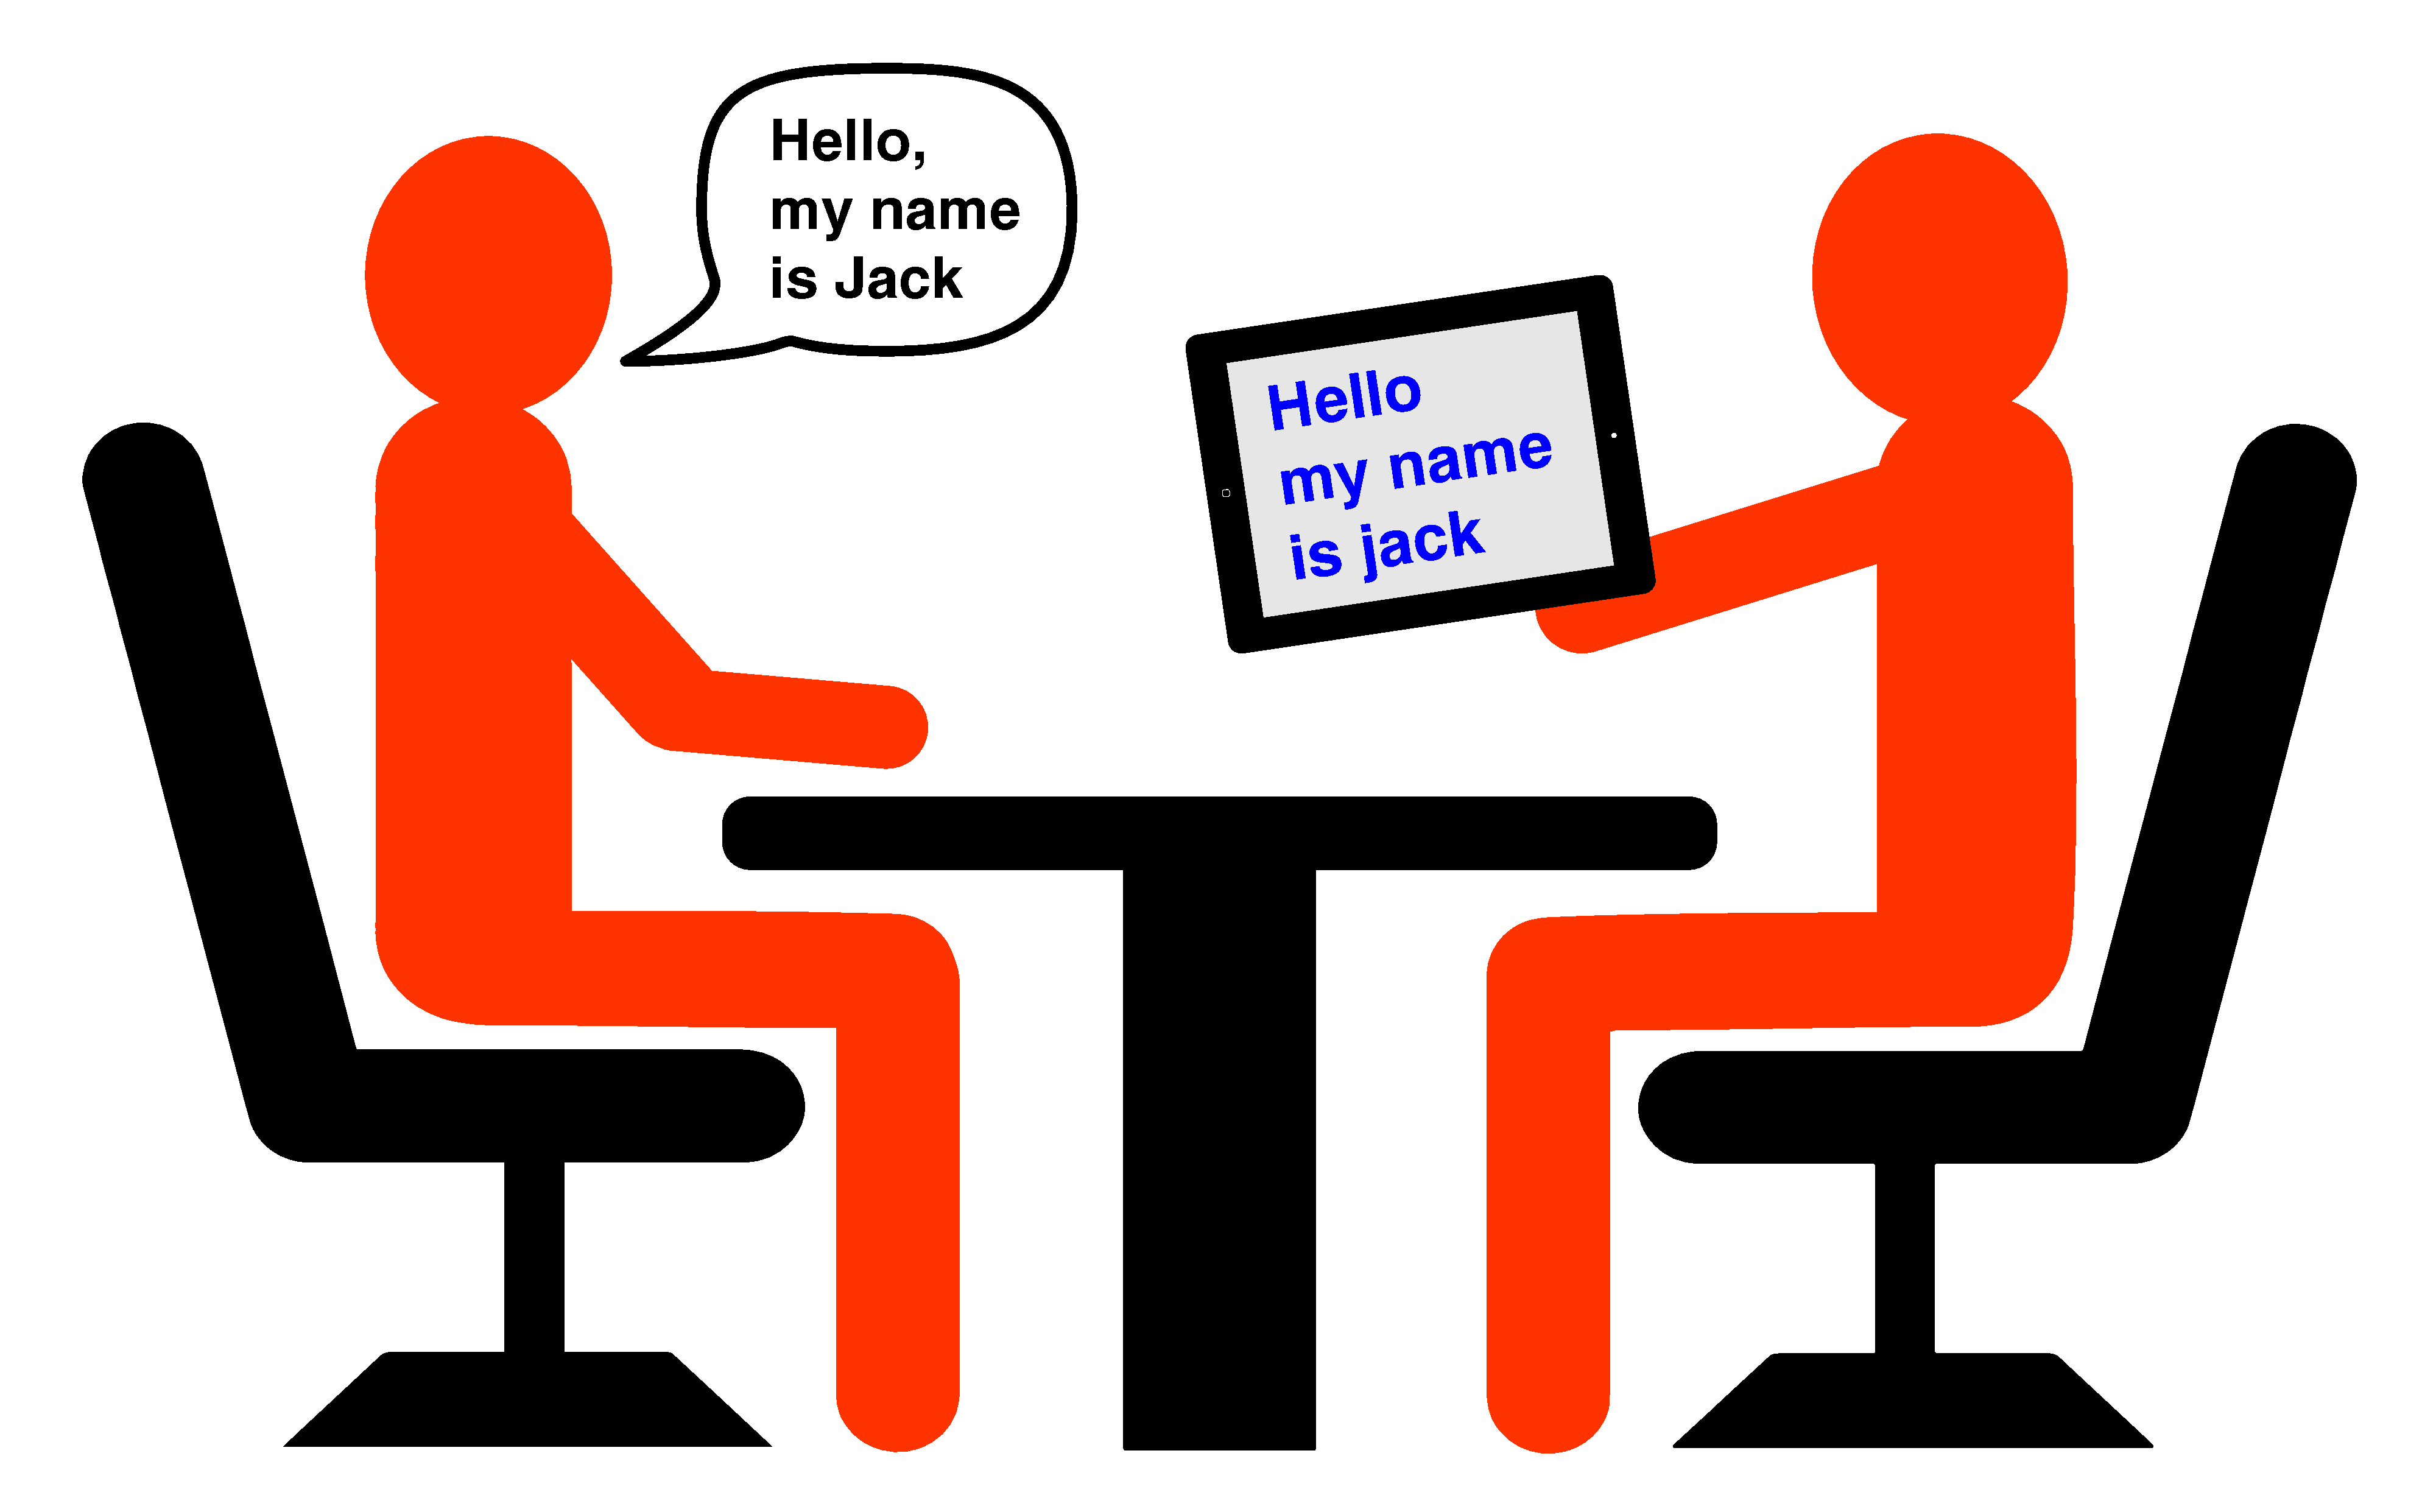
\includegraphics[trim={0cm 0cm 0cm 0cm}, clip, width=\textwidth]{assistant3.pdf}
    \caption{The operation principle and an example use case for the Conversation Assistant. In the illustration, the person on the left is speaking. The person on the right uses the Conversation Assistant, which converts the speech into text in real-time.}
    \label{fig:assistant} 
\end{figure} 
Ideally, the Conversation Assistant could be used with any applicable smart device the user already owns, as long as the basic requirements are met. The Conversation Assistant method is described in detail in section \ref{sec:implementation}. Using automatic speech recognition technology to support deaf and hard of hearing individuals in some form or capacity has been proposed and tested already previously \cite{robison1996computer, kheir2007inclusion, mirzaei2012combining}. However, many of these studies have focused only on some particular setting or situation, such as school classrooms, or have otherwise been limited in their scope. Also, automatic speech recognition technology has matured considerably during this decade, meaning that the findings of many earlier studies might not be accurate any longer. A similar communication aid using Finnish speech recognition was investigated by Karjalainen et al. already in 1997. However, to the extend of our knowledge, no implementations of an application like the Conversation Assistant are currently available for the Finnish language.

\subsection{Problems With Current Solutions}

Some deaf and hard of hearing persons use sign language as an alternative for spoken communication. While this can work well for people who are fluent in it, the problem is that very few people know sign language, especially outside the deaf community. In fact, the share of sign language users among the hearing impaired has been constantly decreasing as a result of modern treatment technology \cite{stacey2006hearing, raino2012sisakorvaistutteen}. In particular, the cochlear implant has enabled a significant share of prelingually\footnote{before language acquisition, including congenital cases (present at birth).} deaf children not to require sign language for communication anymore \cite{moore2007cochlear, peterson2010cochlear}. Different studies estimate that in the near future, approximately 60-80\% of prelingually deaf children will use speech as their primary means of communication, as opposed to sign language, thanks to the improved auditory perception provided by cochlear implants \cite{raino2012sisakorvaistutteen}. As a consequence, the need and incentive for the general public to learn sign language in order to communicate with hearing impaired individuals is diminishing even further. As the technological and medical solutions continue to advance, sign language is slowly becoming obsolete. Indeed, sign language is though to be in danger of becoming extinct in the coming decades \cite{raino2012sisakorvaistutteen}. \\\\
While modern hearing aids and cochlear implants have become very sophisticated by utilizing digital technology and signal processing, there remains many challenges and limitations in their everyday use \cite{levitt2007historical}. One of the major obstacles can be the cost: High-end, personalized devices and surgery are expensive, especially if not covered by health insurance or provided by a public healthcare system \cite{wilson2017global}. Adherence to hearing aid use and rehabilitation can be low: It has been estimated that only 20-50\% of the people who would benefit from a hearing aid are actually using one \cite{koskela2013kuulokojeen}. Even with the extensive digital signal processing and noise reduction in current devices, speech intelligibility in situations with background noise remains one of the major challenges \cite{healy2016difficulty, levitt2007historical, goehring2016speech}. Cochlear implants in particular appear to be very susceptible to noise with a dramatic reduction in speech perception quality in noisy conditions \cite{ healy2016difficulty, friesen2001speech, fu2005noise, srinivasan2013improving}. For public spaces and events, the effects of noise and the environment can be alleviated with a specially installed induction loop, commonly referred to as a \textit{hearing loop} \cite{salonen2013hearing}: The desired sound source is fed electrically into a current-carrying wire loop, and the resulting electromagnetic field containing the baseband audio signal is picked up directly by a hearing aid or other device. The pickup coil in a hearing aid or implant is commonly referred to as the \textit{telecoil} (or \textit{T-coil}). Typical installation locations include airports, auditoriums, concert halls and public bureau buildings. FM systems are a similar alternative for induction loops that use radio transmission instead of electromagnetic induction. Naturally, these solutions are not without some technical and practical complications. Interference from metallic structures and other equipment can be an issue, leading to an uneven field strength and affecting the reception quality. One very concrete problem is that many places don't have them installed (yet) \cite{wilson2017global, healy2016difficulty}. \\\\
Currently, human sign and written language interpreters have a large role in facilitating face-to-face communication between hearing and non-hearing persons, especially in more formal situations that can be scheduled in advance \cite{raino2012sisakorvaistutteen, pereira2010communication, gaur2016effects}. Written language interpreters translate speech to text simultaneously with a speaker by manually typing it into a computer. Written language interpretation happens only in one direction, whereas sign language interpretation can be bidirectional: first, the sign language interpreter translates speech into signs. Then the sign language user can respond with signs, which are then spoken aloud by the translator. Interpreters are used for example in classrooms, meetings, public events and private appointments. Requiring an extra person for communication has many obvious disadvantages \cite{gaur2016effects}. Firstly, there are the multitude of practical challenges, like that interpreters are not available at all times and in all situations. Their number and availability can be quite limited especially outside urban population centers. Professional interpreters typically require a multi-year education and training, limiting their number and introducing costs. Interpretation can lead to a reduced possibility for self-determination \cite{pereira2010communication}. Privacy and communication of sensitive matters can also be a concern, even though interpreters are customarily bound by confidentiality. \\\\
In conclusion, all the existing traditional solutions have their own problems. One of the fundamental issues with many of the above-mentioned are the costs associated with them, both for the individual and for society \cite{wilson2017global}. The proposed ASR-based solution has the potential to be a relatively inexpensive and highly cost-efficient alternative, enabling communication for the hearing impaired in everyday conversational situations quickly and conveniently. Ideally, the Conversation Assistant could also remove the need for human interpreters in many situations, or at least function as a workable alternative when human interpreters are not available.

\subsection{Research Goals}

A lot of research and progress has been made on improving automatic speech recognition technology \cite{yu2014automatic, gales2008application, keronen2014approaching, hinton2012deep, pylkkonen2013towards, xiong2016achieving, enarvi2017automatic}. While technical advancement and knowledge are valuable purely for their own sake, the practical application of this accumulated knowledge is arguably equally important. Correspondingly, the purpose and contribution of this work is to apply the latest developments in ASR into practice, in the hopes of helping with a real-world problem faced by millions of individuals around the world. The main focus of this thesis is on the practical implementation of a proof-of-concept prototype for the Conversation Assistant, as well as user testing the prototype with real users in order to properly validate it as a viable solution. Consequently, designing and performing the necessary user tests for validating the concept and evaluating its usefulness for the end-users also form a major part of this work. Overall, the contents and research goals of this thesis can be framed into four distinct segments:
\vspace{1mm}
\begin{enumerate}[itemsep=2mm]
    \item Understanding the challenges deaf and hard of hearing individuals face in conversational situations.
    \item Developing a proof-of-concept prototype for testing the method.
    \item Planning and carrying out user tests with real intended end-users.
    \item Analysing the results:
    \begin{itemize}[align=left,  leftmargin=0.52cm, labelsep=-0.18cm, itemsep=2mm]
        \item Is the Conversation Assistant a viable concept, and feasible for practical implementation and use?
        \item How the application can, and should be implemented?
        \item What are the main factors for improving its usefulness? 
        \item Is there commercial potential for it? \\
    \end{itemize}
\end{enumerate}

\subsection{Thesis Structure}

This thesis is organized in the following way: Section \ref{sec:tausta} gives an overview of the foundations of this work, providing background information on hearing impairment, automatic speech recognition, software engineering and user testing. It also includes a review of previous work relating to this topic and other proposed solutions for the same problem. Section \ref{sec:implementation} describes the proposed Conversation Assistant method, and presents the design and implementation of the prototype. Likewise, the automatic speech recognition system and the models used are described briefly. In section \ref{sec:testing}, the objectives, design quidelines and choices made for the user test are presented, followed by a detailed description of the resulting test plan and its practical execution. The results from the user testing are presented and analyzed in section \ref{sec:results}. Section \ref{sec:loppu} concludes this thesis. It contains a summary of the work done and results obtained, together with a review whether the objectives set forth in the beginning were met. Finally, conclusions drawn from the results and avenues for future work are discussed.

\clearpage

\section{Background} \label{sec:tausta}

This section presents the theory and scientific context behind the work. Developing and testing the Conversation Assistant is a multidisciplinary task requiring knowledge from a variety of fields from computer science and software engineering to medicine and psychology. Since an assistive software-based solution is being developed specifically for deaf and hard of hearing individuals, comprehensive knowledge of hearing and hearing loss is required so that the problem being solved can be understood, and the factors affecting it taken into account. Likewise, it is equally important to possess a general overview of currently existing assistive solutions, in order to understand and assess the Conversation Assistant's place and impact in the big picture. Information on the social impact of hearing impairment and the problems hearing impaired individuals face on a daily basis offer a clear-cut motivation and reason for the work presented. Additionally, it is relevant to know the demographics of hearing impairment in order to asses the scope of the problem and the scale needed for potential solutions, of which a very concrete example would be for instance how many web servers could potentially be needed for a cloud-based speech recognition application. The number of hearing impaired individuals also directly affects the demand and commercial potential for the presented software solution. Functioning of the Conversation Assistant is based on automatic speech recognition, and therefore, it is necessary to understand how an ASR system works. The main goal of this work is to develop a software application that answers to the needs of the target user group as well as possible. Succeeding in this goal requires the discipline of software engineering, especially in the form of user-centered design and engineering. Overall, these contents form the theoretical framework enabling the design, engineering and testing of the Conversation Assistant. \\\\
The contents of this section are divided as follows: Section \ref{subsec:hear} presents a review of hearing impairment, including the physiological mechanisms, prevalence, and societal impact. In addition, existing treatments and assistive technology is covered briefly. Section \ref{subsec:asr} presents the theory and operation of automatic speech recognition systems, and section \ref{subsec:soft} describes the principles of software development and user testing as related to this thesis. Previous work relating to this particular topic and other proposed technological solutions are reviewed in section \ref{subsec:work}.

\subsection{Hearing Impairment} \label{subsec:hear}

Unlike many other disability groups, hearing impaired people are a highly heterogeneous group with different types and levels of hearing impairment \cite{cavender2008hearing}. There are some for whom sign language is their primary, or even possibly their only language, and conversely, there are many who do not know or use sign language at all \cite{raino2012sisakorvaistutteen}. Some are born deaf, while others can suffer from hearing loss later in life due to an illness, accident or through exposure to noise \cite{moore2007cochlear}. Age-related hearing loss is common for the elderly, even though many of them do not identify themselves as hearing impaired \cite{salonen2013hearing}. Typically, the term \textit{hard of hearing} is used to refer to individuals with some degree of hearing still present and still communicating mostly through spoken language \cite{deafness}. The term \textit{deaf} generally refers to people with very little or no hearing ability at all, often using sign language for communication \cite{deafness}. Hearing loss can be an invisible disability, and there remains some social stigma associated with it. Individuals with hearing loss often try to hide it, as it sometimes perceived to be associated with ageing or low intelligence \cite{wilson2017global, salonen2013hearing}. Access to modern assistive devices and treatment remains limited for many people, even in the developed countries: The high cost of hearing aids and cochlear implants means that many people who could benefit from them cannot afford one \cite{wilson2017global}.

\subsubsection{Definition}

Hearing impairment can be defined as having a reduced or deficient hearing ability, generally caused as a result of decreased hearing sensitivity in one or both ears \cite{moore2007cochlear, ohlenforst2017effects}. Neurological conditions affecting auditory processing in the brain have also been identified, though they are quite rare and hard to diagnose. These \textit{auditory processing disorders} show as various difficulties in recognizing and interpreting sounds correctly, even though the ears are functioning physiologically normally \cite{deafness}. The terms \textit{hearing impairment} and \textit{hearing loss} ar commonly used synonymously \cite{moore2007cochlear}. In this work, \textit{hearing loss} is used to refer specifically to sensory impairment of hearing, and \textit{hearing impairment} to the overall condition and disability resulting from auditory dysfunctions. \\\\
Clinically, hearing loss can be divided into two main categories based on the physiological cause \cite{moore2007cochlear, deafness}: Conductive hearing loss is a result of abnormalities in the outer ear or in the ossicles in the middle ear, with the effect that sound is not properly transmitted to the inner ear. Sensorineural hearing loss results from a malfunction of the inner ear or the auditory nerve, meaning that the problem is in converting sound vibration into neural impulses and transmitting them to the auditory cortex of the brain. For example, damage to the hair cells in the cochlea is a common form of sensorineural hearing loss \cite{moore2007cochlear}. The anatomy of the ear is presented in figure \ref{fig:ear}, describing the parts belonging to the outer, middle, and inner ear. \\\\
The overwhelming majority of all hearing impairments are of the sensorineural type, with age-related hearing loss, or \textit{presbycusis}, being the most common cause, followed by noise-induced hearing loss \cite{koskela2013kuulokojeen}. It is possible to have a combination of both conductive and sensorineural hearing defects as well. Another significant division for hearing loss and its treatment is the age of onset in relation to speech acquisition \cite{raino2012sisakorvaistutteen, deafness}: Prelingual hearing loss is present before language acquisition, meaning it is either congenital (present at birth) or develops soon after. Postlingual hearing loss occurs after the development of speech and language. This distinction is important since deafness and hearing loss can significantly affect the language acquisition of children, a fundamental part of general cognitive development \cite{moore2007cochlear, wilson2017global, raino2012sisakorvaistutteen}.
\begin{figure}[t]
    \centering 
    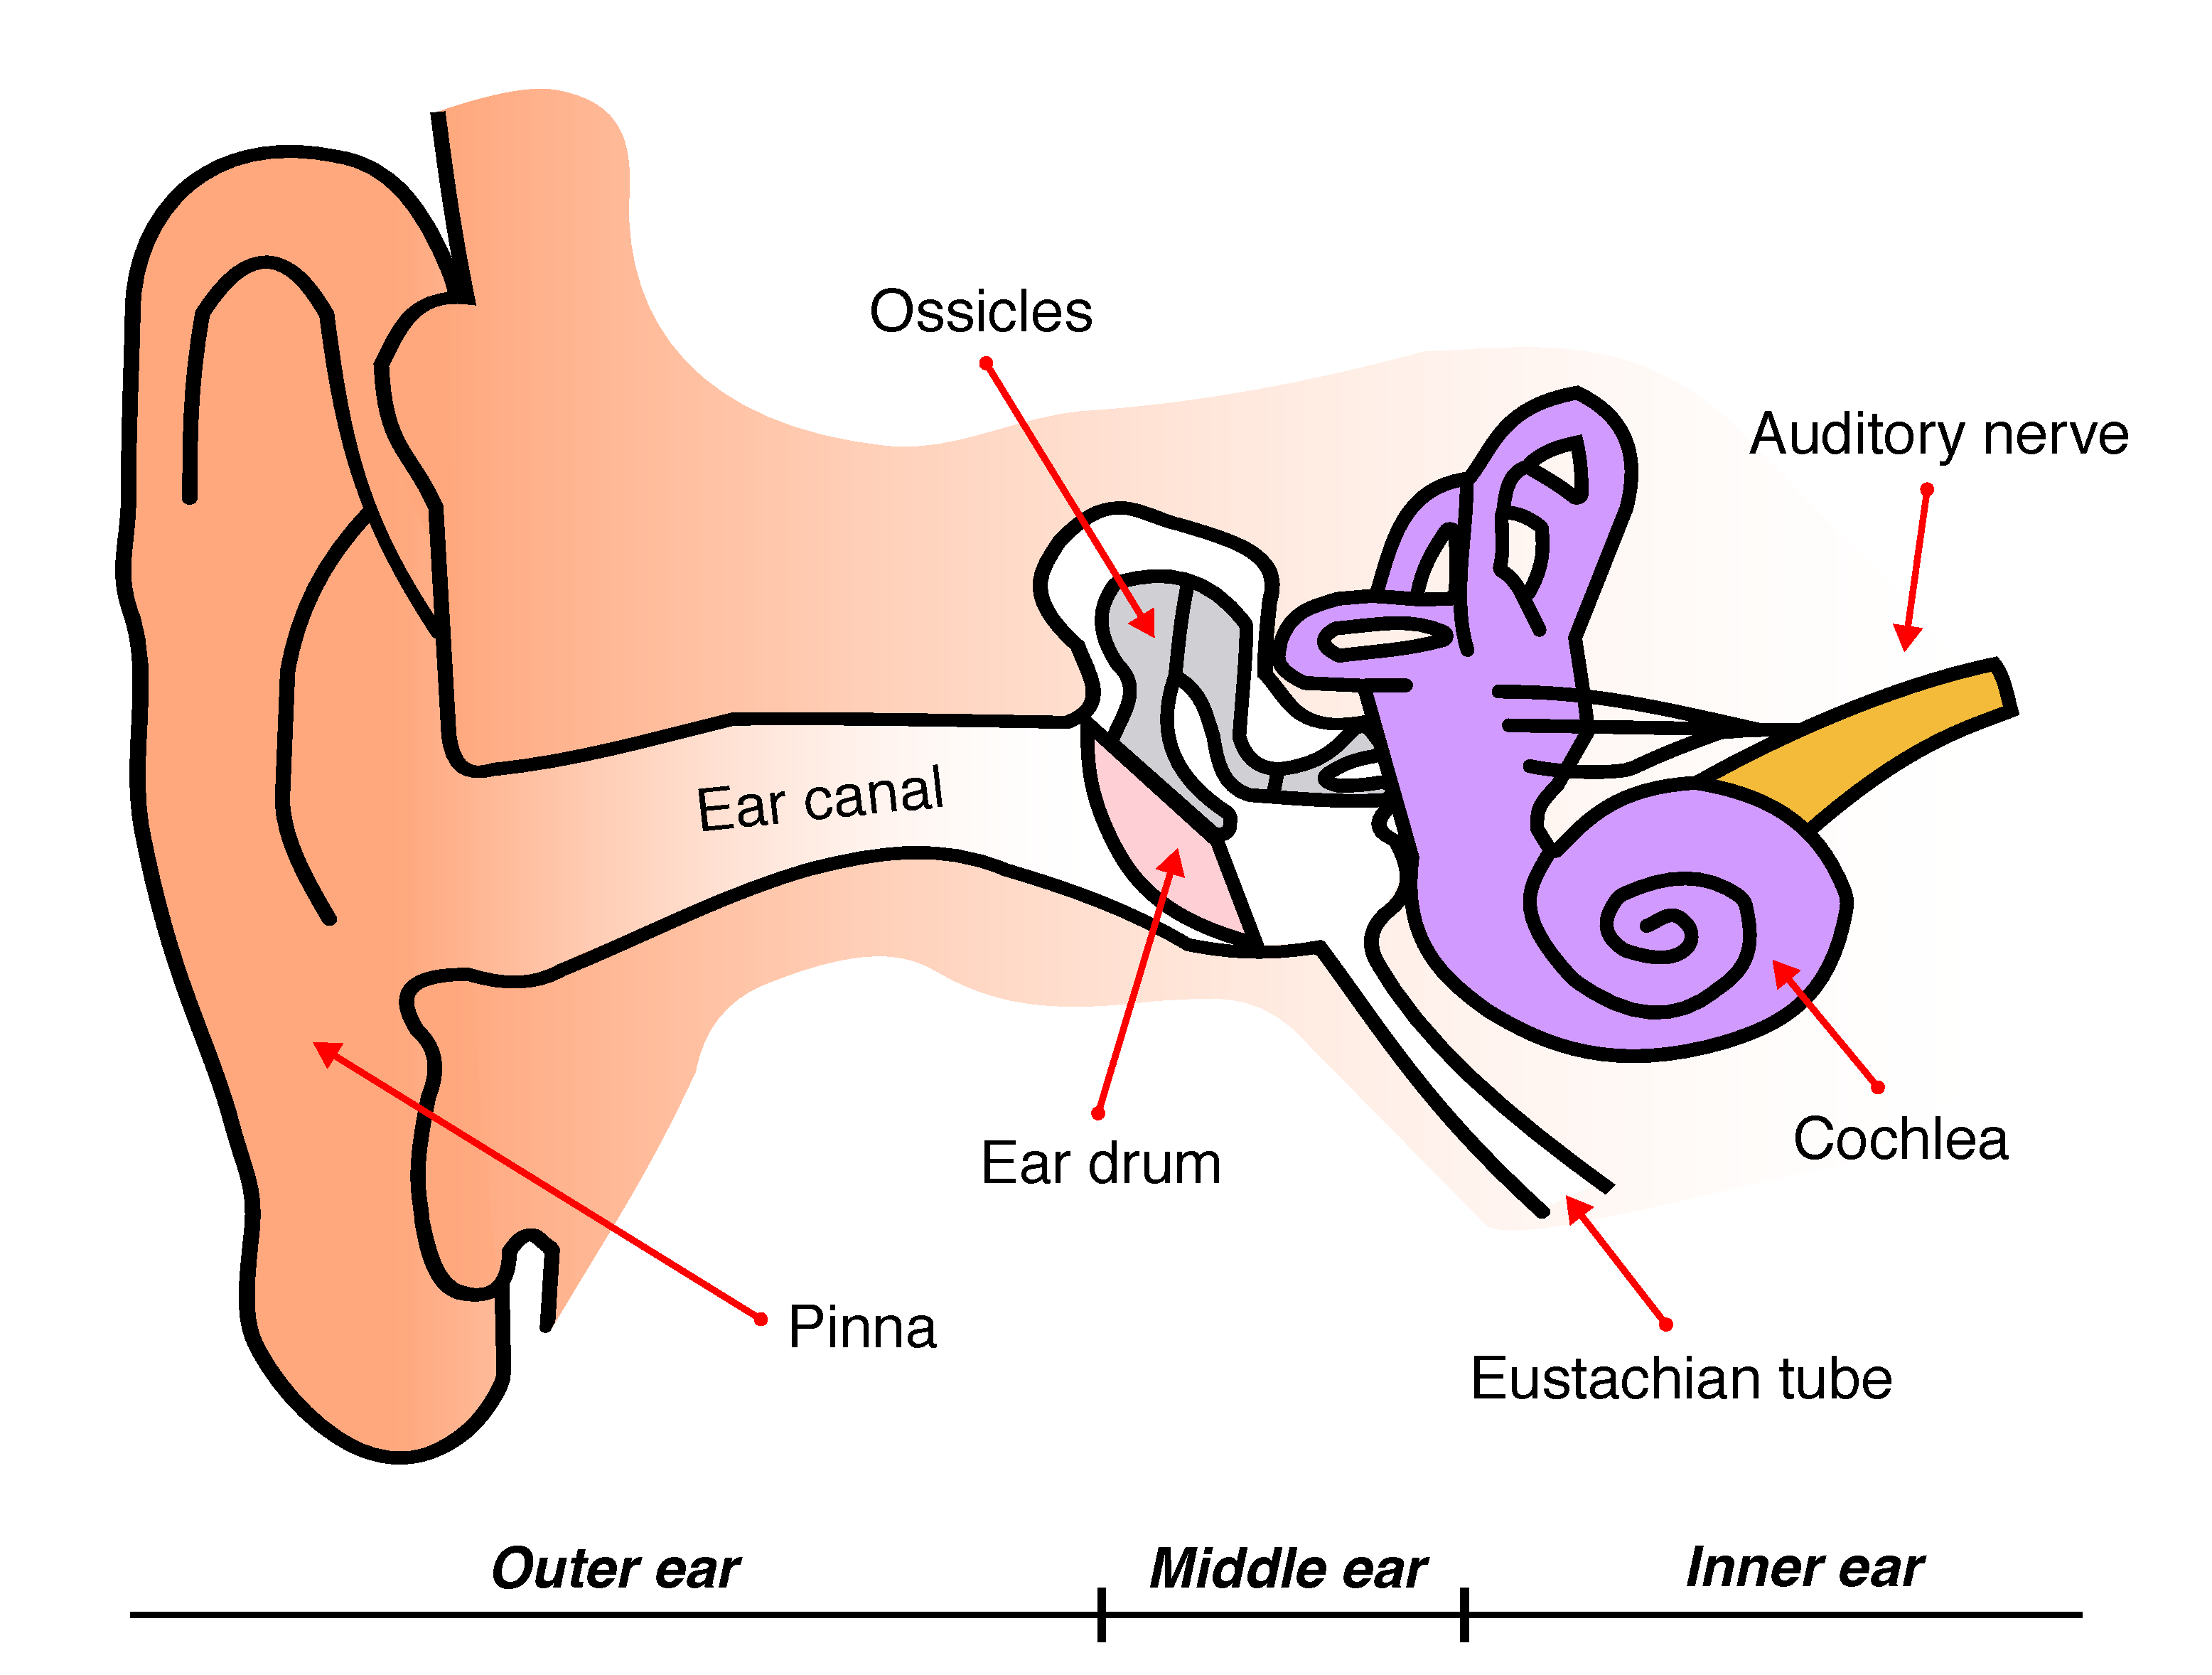
\includegraphics[width=\textwidth]{ear.pdf}
    \caption{Anatomy of the ear. The outer ear consists of the pinna and the ear canal, ending to the eardrum (tympanic membrane). The middle ear is a small air-filled cavity containing the ossicles: three tiny bones responsible for transmitting the vibration of the eardrum to the inner ear. The Eustachian tube is a narrow channel connecting the middle ear to the oral cavity, balancing the air pressure inside to the external air pressure. The inner ear houses the cochlea, a spiral-shaped liquid-filled tube containing the basilar membrane, along which the hair cells are positioned. Hair cells convert the vibration of the basilar membrane into neural impulses in the auditory nerve. \cite{moore2007cochlear, pulkki2015communication}}
    \label{fig:ear} 
\end{figure} \\
Audiologically\footnote{Audiology is the scientific study of hearing, including the treatment of hearing defects.}, hearing loss is categorized and its severity ranked according to the increase in the threshold of hearing, i.e., the sound pressure level required for the perceptual detection of sound \cite{moore2007cochlear, pulkki2015communication}. It is measured in decibels and compared to the statistically defined and standardized nominal level of hearing. Human hearing is strongly frequency-dependent, and is most sensitive at frequencies from approximately one to five kilohertz \cite{pulkki2015communication}. Consequently, this frequency range is critical for speech perception and many other everyday tasks. Figure \ref{fig:loudness} presents the equal-loudness contours as they are defined in the ISO 226:2003 standard \cite{iso226}. These contours describe the \textit{sound pressure level} (SPL) required for a pure tone (single frequency sinusoidal waveform) to be judged equally loud depending on the frequency of the tone, illustrating the frequency-dependent sensitivity of hearing \cite{pulkki2015communication}. Notably, the equal-loudness curve for zero phons corresponds to the absolute threshold of hearing. Hearing loss can therefore be technically defined as upward changes to this curve, the frequency-dependent threshold of hearing, that exceed the normal small statistical variation between different people. \\
\begin{figure}[]
    \centering 
    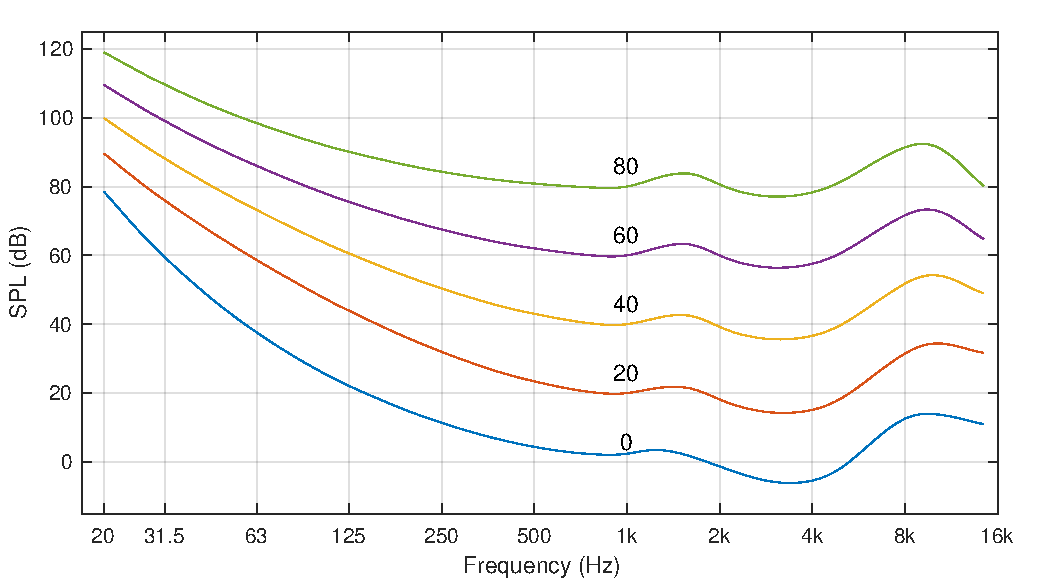
\includegraphics[width=\textwidth]{loudness.pdf}
    \caption{Equal-loudness contours as defined in ISO 226:2003. The number associated with each curve is the nominal loudness level in phons, with zero phons corresponding to the nominal threshold of hearing. Sound pressure level is the pressure level compared to the reference value of \ $ \mathit{20 \cdot 10^{-6}}$ Pascals. \cite{iso226}}
    \label{fig:loudness} 
\end{figure} \\
The level of hearing loss is generally described as a single decibel value, referred to as the \textit{pure tone average} (PTA) \cite{moore2007cochlear, salonen2013hearing}. It is calculated as the average of the hearing thresholds for pure tones at the frequencies of 0,5 kHz, 1 kHz, 2 kHz, and 4 kHz: For each frequency, the threshold of hearing is measured and compared to the reference value, resulting in a decibel value, which are then averaged together to form a single value estimate. Different severity categories have been set up with each category having a corresponding decibel range of the average hearing threshold increase. These decibel ranges vary slightly between countries and organizations \cite{salonen2013hearing}. Table \ref{table:hearingloss} presents two common severity ranks, and the corresponding decibel ranges for the pure tone average used by the \textit{World Health Organization} (WHO) and the \textit{European Working Group on Genetics of Hearing Impairment} (EUWG) \cite{salonen2013hearing}. \\\\
However, this does not mean that all individuals in the same category or even with the same pure tone average value have the same effective hearing impairment: Difficulties for instance with speech perception can vary widely depending on how much each frequency is affected and the mechanisms causing the hearing loss. People with mild or moderate hearing loss can typically understand speech reasonably well in a quiet room with only one person talking. However, they can begin to have difficulties when more than one person is talking at the same time, or when there is background noise or notable reverberation present \cite{peterson2010cochlear}. People with severe or profound hearing loss usually have difficulties even with understanding a single speaker in a quiet room, and severe problems when background noise is present. In addition to decreased audibility, hearing impairment typically causes additional perceptual difficulties not purely related to the reduced sensitivity \cite{moore2007cochlear}: The frequency resolution of hearing is often also affected, leading to the significant difficulties with speech perception in noisy conditions. \\\\
Humans are normally very good at understanding speech in noise, and can concentrate on a specific speaker or audio source among many other competing sound sources. This is typically referred to as the \textit{cocktail party effect} \cite{bronkhorst2000cocktail}. In hearing loss, the auditory filters of the ear that divide the incoming sounds into different frequency bands can become wider and more shallow due to damage to the hair cells \cite{moore2007cochlear}. This leads to increased auditory masking of adjacent frequencies, where one sound interferes with the detection of another sound. Also, the level of hearing loss typically varies between the ears, with one ear being better than the other. This affects the binaural processing of hearing, which is important for instance for sound localization, i.e., the detection of the direction and distance of sound sources \cite{moore2007cochlear, pulkki2015communication}. The end result is that the auditory system is unable to effectively isolate speech from noise, meaning that simply amplifying all sound does not help \cite[p.~233--234]{moore2007cochlear}. Instead, the \textit{signal-to-noise ratio} (SNR), the ratio between the level of the desired audio signal and the level of background noise needs to be improved considerably for better speech intelligibility in noisy conditions \cite{healy2016difficulty, fink2008benefit}.
\begin{table}[t]
    \renewcommand{\arraystretch}{1.2}  % set row height to 1.2x default
    \setlength{\tabcolsep}{32pt}                % set space between text and cell border
    \centering
    \caption{Categories for the grade of hearing loss and corresponding pure tone average ranges as defined by WHO and EUWG \cite{salonen2013hearing}.}
    \label{table:hearingloss}
    \begin{tabular}{@{}lll@{}}
        \toprule
        & \textbf{WHO}  & \textbf{EUWG}                                 \\ \midrule
        Severity        & \multicolumn{2}{l}{Pure Tone Average (dB HL)} \\ \midrule
        Normal          & 0-25                      & 0-19              \\
        Mild            & 26-40                     & 20-39             \\
        Moderate        & 41-60                     & 40-69             \\
        Severe          & 61-80                     & 70-94             \\
        Profound        & $\geqslant$ 81            & $\geqslant$ 95    \\ \bottomrule
    \end{tabular}
    \vspace{2mm}
\end{table}

\subsubsection{Prevalence}

In this case, prevalence is defined as the percentage of a population that is affected by hearing loss. A pure tone average greater than 25 dB HL in both ears is defined as a disabling hearing loss by WHO criteria, as exceeding this level begins to clearly impair communication in daily life \cite{salonen2013hearing}. Most population studies use this number for defining hearing impairment \cite{salonen2013hearing, lin2011hearing}. From a public health perspective,  hearing impairment can be considered a major health and economic problem: Approximately 0,1 - 0,3\% of newborn children have hearing impairment, while over 50 percent of the population over 75 years of age has a hearing loss requiring treatment \cite{salonen2013hearing}.  \\\\
In Finland, an estimated eleven percent of the workforce \cite{koskela2013kuulokojeen}, and around 15-18\% of the whole adult population has some degree of hearing loss \cite{salonen2013hearing}. The prevalence of hearing impairment among the elderly is high: A Finnish study with 4067 participants found that for the age groups 70, 75, 80, and 85 years, the prevalence for at least a mild hearing loss varied between 37,7\% - 54,1\%, and between 21,1\% - 38,9\% for a moderate or more severe hearing loss \cite{salonen2013hearing}. Among this group, hearing aids were used daily by 55,4\% of the 249 persons who responded to a mailed interview. \\\\
In the USA, Lin et al. \cite{lin2011hearing} estimated in 2011, based on data from 2001 to 2008, that 30.0 million or 12.7\% of Americans aged 12 years or older had bilateral hearing loss, increasing to 48.1 million or 20.3\% when individuals with unilateral hearing loss were included. Overall, they found hearing loss to increase with every age decade, with the prevalence of hearing loss expected to rise because of an aging population. \\\\
According to the WHO Global Burden of Disease study of 2015 \cite{wilson2017global}, approximately half a billion people have disabling hearing loss globally, which corresponds to 6,8\% of the whole world's population. Wilson et al. \cite{wilson2017global} report that these numbers are substantially higher than estimates published before 2013, pointing to the growing importance of hearing loss as a disability, and the need for greater attention to global hearing health care.

\subsubsection{Assistive devices}

The main technological solutions to hearing loss can be divided into three main categories: hearing aids, cochlear implants, and other assistive devices \cite{moore2007cochlear}. Hearing aids are used in mild to severe cases to augment a reduced hearing ability \cite{moore2007cochlear, levitt2007historical}. A cochlear implant is required when hearing aids cannot help anymore, in cases of profound or total hearing loss \cite{moore2007cochlear, levitt2007historical}. Other assistive devices include both supplementary techniques for hearing augmentation, and a wide variety of methods and gadgets based on visual perception and physical interaction. For additional hearing assistance, the previously mentioned audio induction loop and FM system are the most common and widely used, and many hearing aids and cochlear implants have a build-in receiver for these devices. Examples of the latter category include alarm systems using flashing lights instead of sound for applications such as smoke detectors and door bells. A typical example of an assistive device substituting sound with physical interaction is an alarm clock using vibration for awaking a deaf person \cite{mielke2013assistive}. Hearings aids and cochlear implants are being actively developed, and have improved remarkably during the past few decades, though neither device can match the performance of normally functioning hearing \cite{moore2007cochlear, levitt2007historical, goehring2016speech}. More traditional support methods are still being used as well: Lip reading is utilized by many hearing impaired individuals for understanding speech in conjunction with the modern assistive devices. \\\\
Hearing aids are used to amplify and modify incoming sound, enhancing and augmenting the user's own compromised hearing \cite{levitt2007historical, salonen2013hearing, fink2008benefit}. Modern devices are based on digital electronics and microprocessors, and come in many different types. The most common variations are the different \textit{in-the-ear} and \textit{behind-the-ear} models. Figure \ref{fig:hearingaids} presents various types of modern hearings aids from one particular manufacturer (Widex). In addition to the simple amplification provided by earlier analog models, modern digital hearing aids utilize real-time \textit{digital signal processing} (DSP) for tasks such as speech enhancement, dynamics processing (compression), filtering, noise reduction, adaptive gain control and feedback cancellation \cite{moore2007cochlear, levitt2007historical, goehring2016speech}. Directional microphone systems are used for improving speech recognition in noise \cite{levitt2007historical}. Modern wireless transmission technology, such as Bluetooth, can be used to easily link hearing aids directly with sound sources like a telephone or television \cite{salonen2013hearing}. Modern hearing aids are personally fitted for each user, matching and compensating for the individual frequency response of the users hearing for best results \cite{moore2007cochlear}. \\
\begin{figure}[b]
    \centering 
    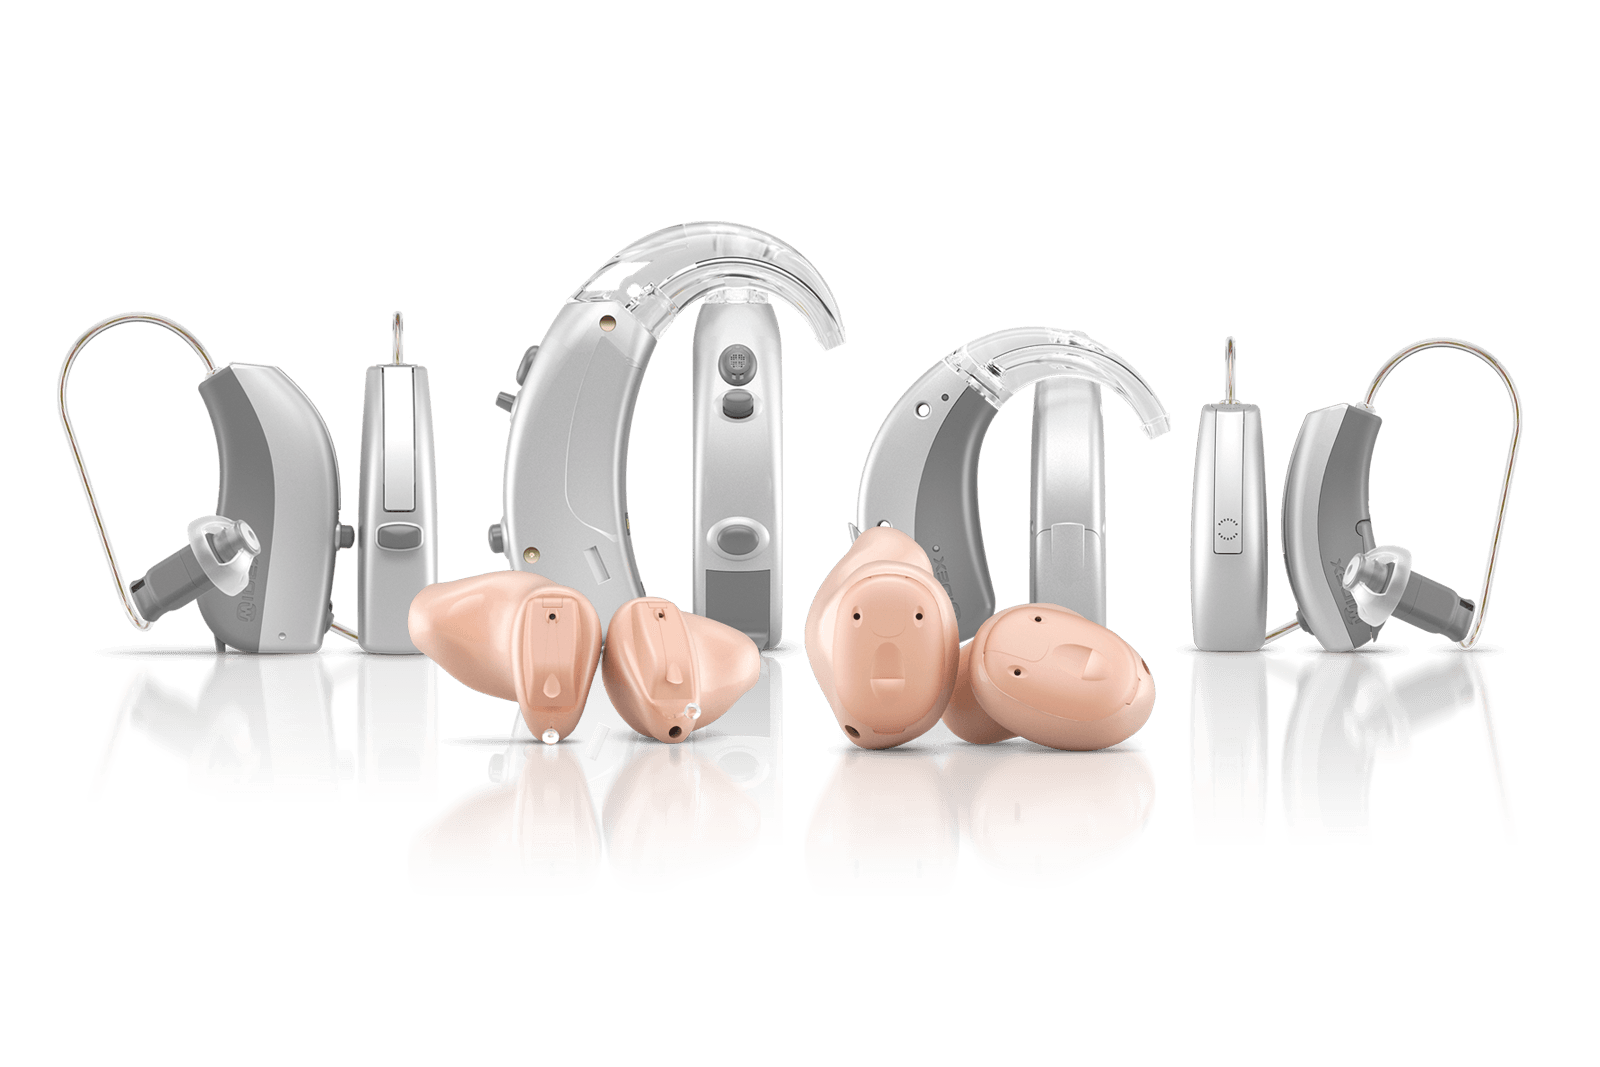
\includegraphics[trim={0cm 4cm 0cm 4cm}, clip, width=\textwidth]{hearingaids.png}   % trim={<left> <lower> <right> <upper>}
    \caption{Different types of modern hearing aids: behind-the-ear (back, middle), receiver-in-canal (back, left and rightmost), in-the-canal (front, left) and in-the-ear (front, right). Image source: \href{https://www.widex.pro/en/products/unique-hearing-aids}{\textit{Widex}}}
    \label{fig:hearingaids} 
\end{figure} \\
A cochlear implant is a surgically implanted electronic device that can provide auditory perception to people with severe or profound sensorineural hearing loss, even in the case of complete deafness \cite{moore2007cochlear, peterson2010cochlear}. Cochlear implants bypass the ear altogether by directly stimulating the auditory nerve with electrical signals through electrodes inserted into the cochlea. All implants are comprised of two major elements: The external, detachable parts, and the internal, surgically implanted parts. The external parts are usually removed for activities such as sleeping and bathing \cite{peterson2010cochlear}. \\\\
Similarly to hearing aids, the audio signal is acquired with an external microphone or picked up wirelessly. The signal is then processed with a speech processor unit typically worn behind the ear. It is transmitted wirelessly through the skin to the internal implant. The internal, implanted part consists of a receiver and the electrodes. The placement of these components is illustrated in figure \ref{fig:implant}, which presents the same anatomic view of the ear as in figure \ref{fig:ear}, but with an added cochlear implant: \\
\begin{figure}[h]
    \centering 
    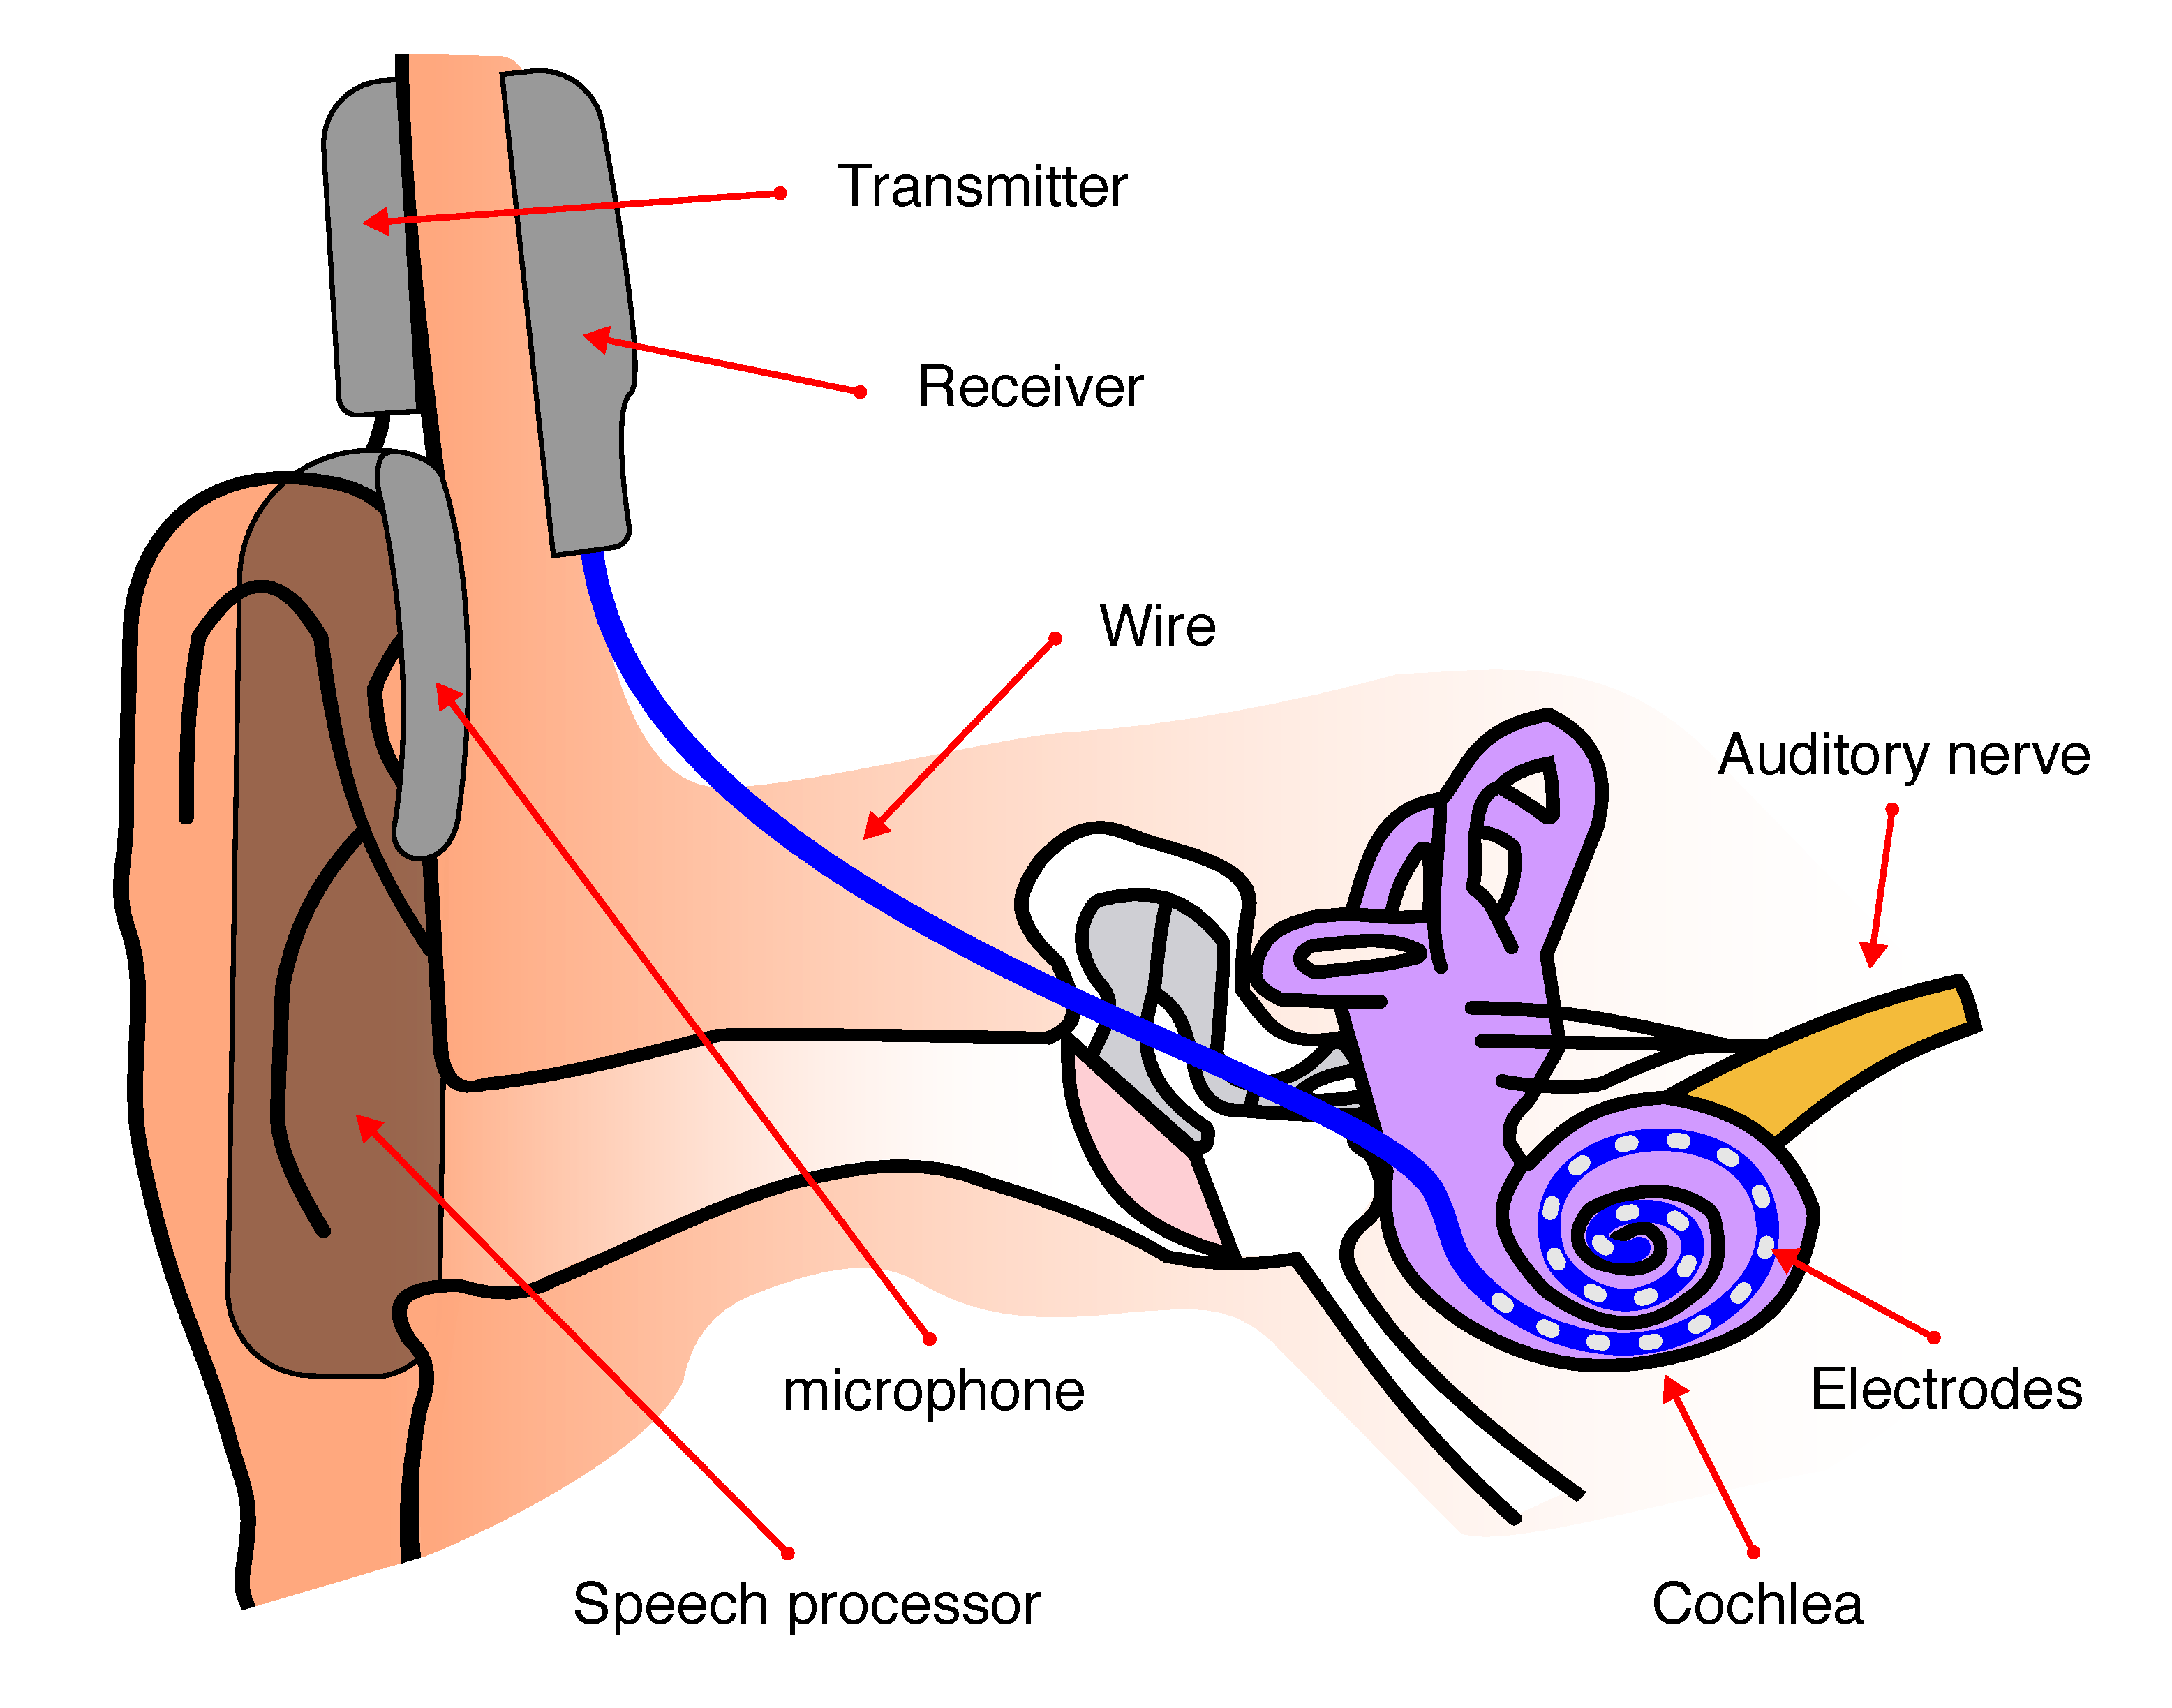
\includegraphics[width=\textwidth]{implant.pdf}
    \vspace{0.5mm}
    \caption{An ear with a cochlear implant. A microphone and speech processor are typically worn behind ear. The speech processor connects to a wireless transmitter attached outside the head. An internal receiver inside the skin connects to the electrodes inserted into the cochlea. \cite{moore2007cochlear, peterson2010cochlear}}
    \label{fig:implant} 
\end{figure} \\
Most cochlear implants are multi-channel, meaning they have multiple electrodes. The input signal is likewise divided into multiple frequency bands with each electrode receiving its own signal \cite{moore2007cochlear, friesen2001speech}. While they do not restore normal hearing sensation, cochlear implants enable speech communication for many recipients and significantly improve the spoken language acquisition for deaf children \cite{stacey2006hearing, raino2012sisakorvaistutteen}: Many congenitally deaf cochlear implant recipients achieve a good speech perception ability and develop near-normal language skills. Post-lingually deafened implant recipients often regain the ability to understand and use spoken language at least to some degree. Cochlear implants have been shown to considerably improve the perceived quality of life for many recipients \cite{blomberg2012sisakorvaistutetta}. \\\\
Cochlear implants are a relatively new treatment method: In Finland, the first few implants were installed in the mid 80s to adults. The first child was implanted in 1995 and the first congenitally deaf child in 1997 \cite{raino2012sisakorvaistutteen}. Today, the majority of prelingually deaf children are implanted already around the age of one year, as the early age of implantation is strongly associated with successful outcomes \cite{peterson2010cochlear, stacey2006hearing, raino2012sisakorvaistutteen}.

\subsubsection{Social impact}

Hearing loss can cause profound social problems and greatly affect an individuals physical and psychological well-being as a consequence of the difficulty with spoken communication and social interaction \cite{wilson2017global, koskela2013kuulokojeen}. The effects of hearing loss can lead to social isolation and stigmatization, depression, and problems with self esteem and work capacity \cite{wilson2017global, koskela2013kuulokojeen, lavikainen2014}. Coping with hearing loss can be challenging, and consequently, psychological illnesses have been found to be more prevalent for the hearing impaired than for those in the general population \cite{wilson2017global}. On a personal level, the quality of life of an individual is ultimately impacted \cite{blomberg2012sisakorvaistutetta}. From a societal and public economy viewpoint, the consequences of hearing loss appear as productivity losses, employment issues, health care and social benefit expenditures, and reduced tax revenue  \cite{wilson2017global}. \\\\
Employment issues is one of the major obstacles hearing impaired people face in society \cite{hietala2008huonokuuloinen}. In Finland, the unemployment rate of people with hearing impairment varied from 30 to 40 percent between the years 1995 and 2002 \cite{hietala2008huonokuuloinen}. For young adults with hearing impairment, the unemployment rate was reported to be twice the rate of the normally hearing population in the same age group \cite{hietala2008huonokuuloinen}. \\\\
Employed hearing impaired people have been observed to have noticeable problems with coping at work and workplace well-being \cite{wilson2017global, hietala2008huonokuuloinen}. The increased listening effort associated with hearing loss, particularly in noisy environments, can be tiring and cause stress \cite{ohlenforst2017effects, koskela2013kuulokojeen}. The negative effects of hearing loss are focused particularly to the ageing workforce \cite{koskela2013kuulokojeen}. Consequently, there appears to be a clear statistical connection between hearing loss and early retirement \cite{hietala2008huonokuuloinen}.

\clearpage

\subsection{Automatic Speech Recognition} \label{subsec:asr}

In this work, the primary interest in automatic speech recognition is for using it in practice, instead of developing or improving upon some aspect of it. Therefore, this section focuses on providing a high-level overview of ASR systems. Likewise, detailed description of machine learning techniques and neural network training methods fall outside this thesis. In this work, speech recognition is described primarily from the point of view of modern large vocabulary continuous speech recognition. \\\\ An automatic speech recognition system takes an audio signal containing speech as an input, and tries to produce the corresponding text representation \cite{huang2001spoken, li2014overview}. Figure \ref{fig:asr} presents the high-level block diagram of a typical speech recognition system, though other configurations are also possible. In practice, the actual implementation can typically contain more complicated connections between the different components, and the models can also be packed together for optimization reasons \cite{yu2014automatic, kallasjoki2016}. The use of deep neural networks has somewhat blurred the line between feature extraction and acoustic modeling \cite{hinton2012deep, kallasjoki2016}.
\begin{figure}[h]
    \centering 
    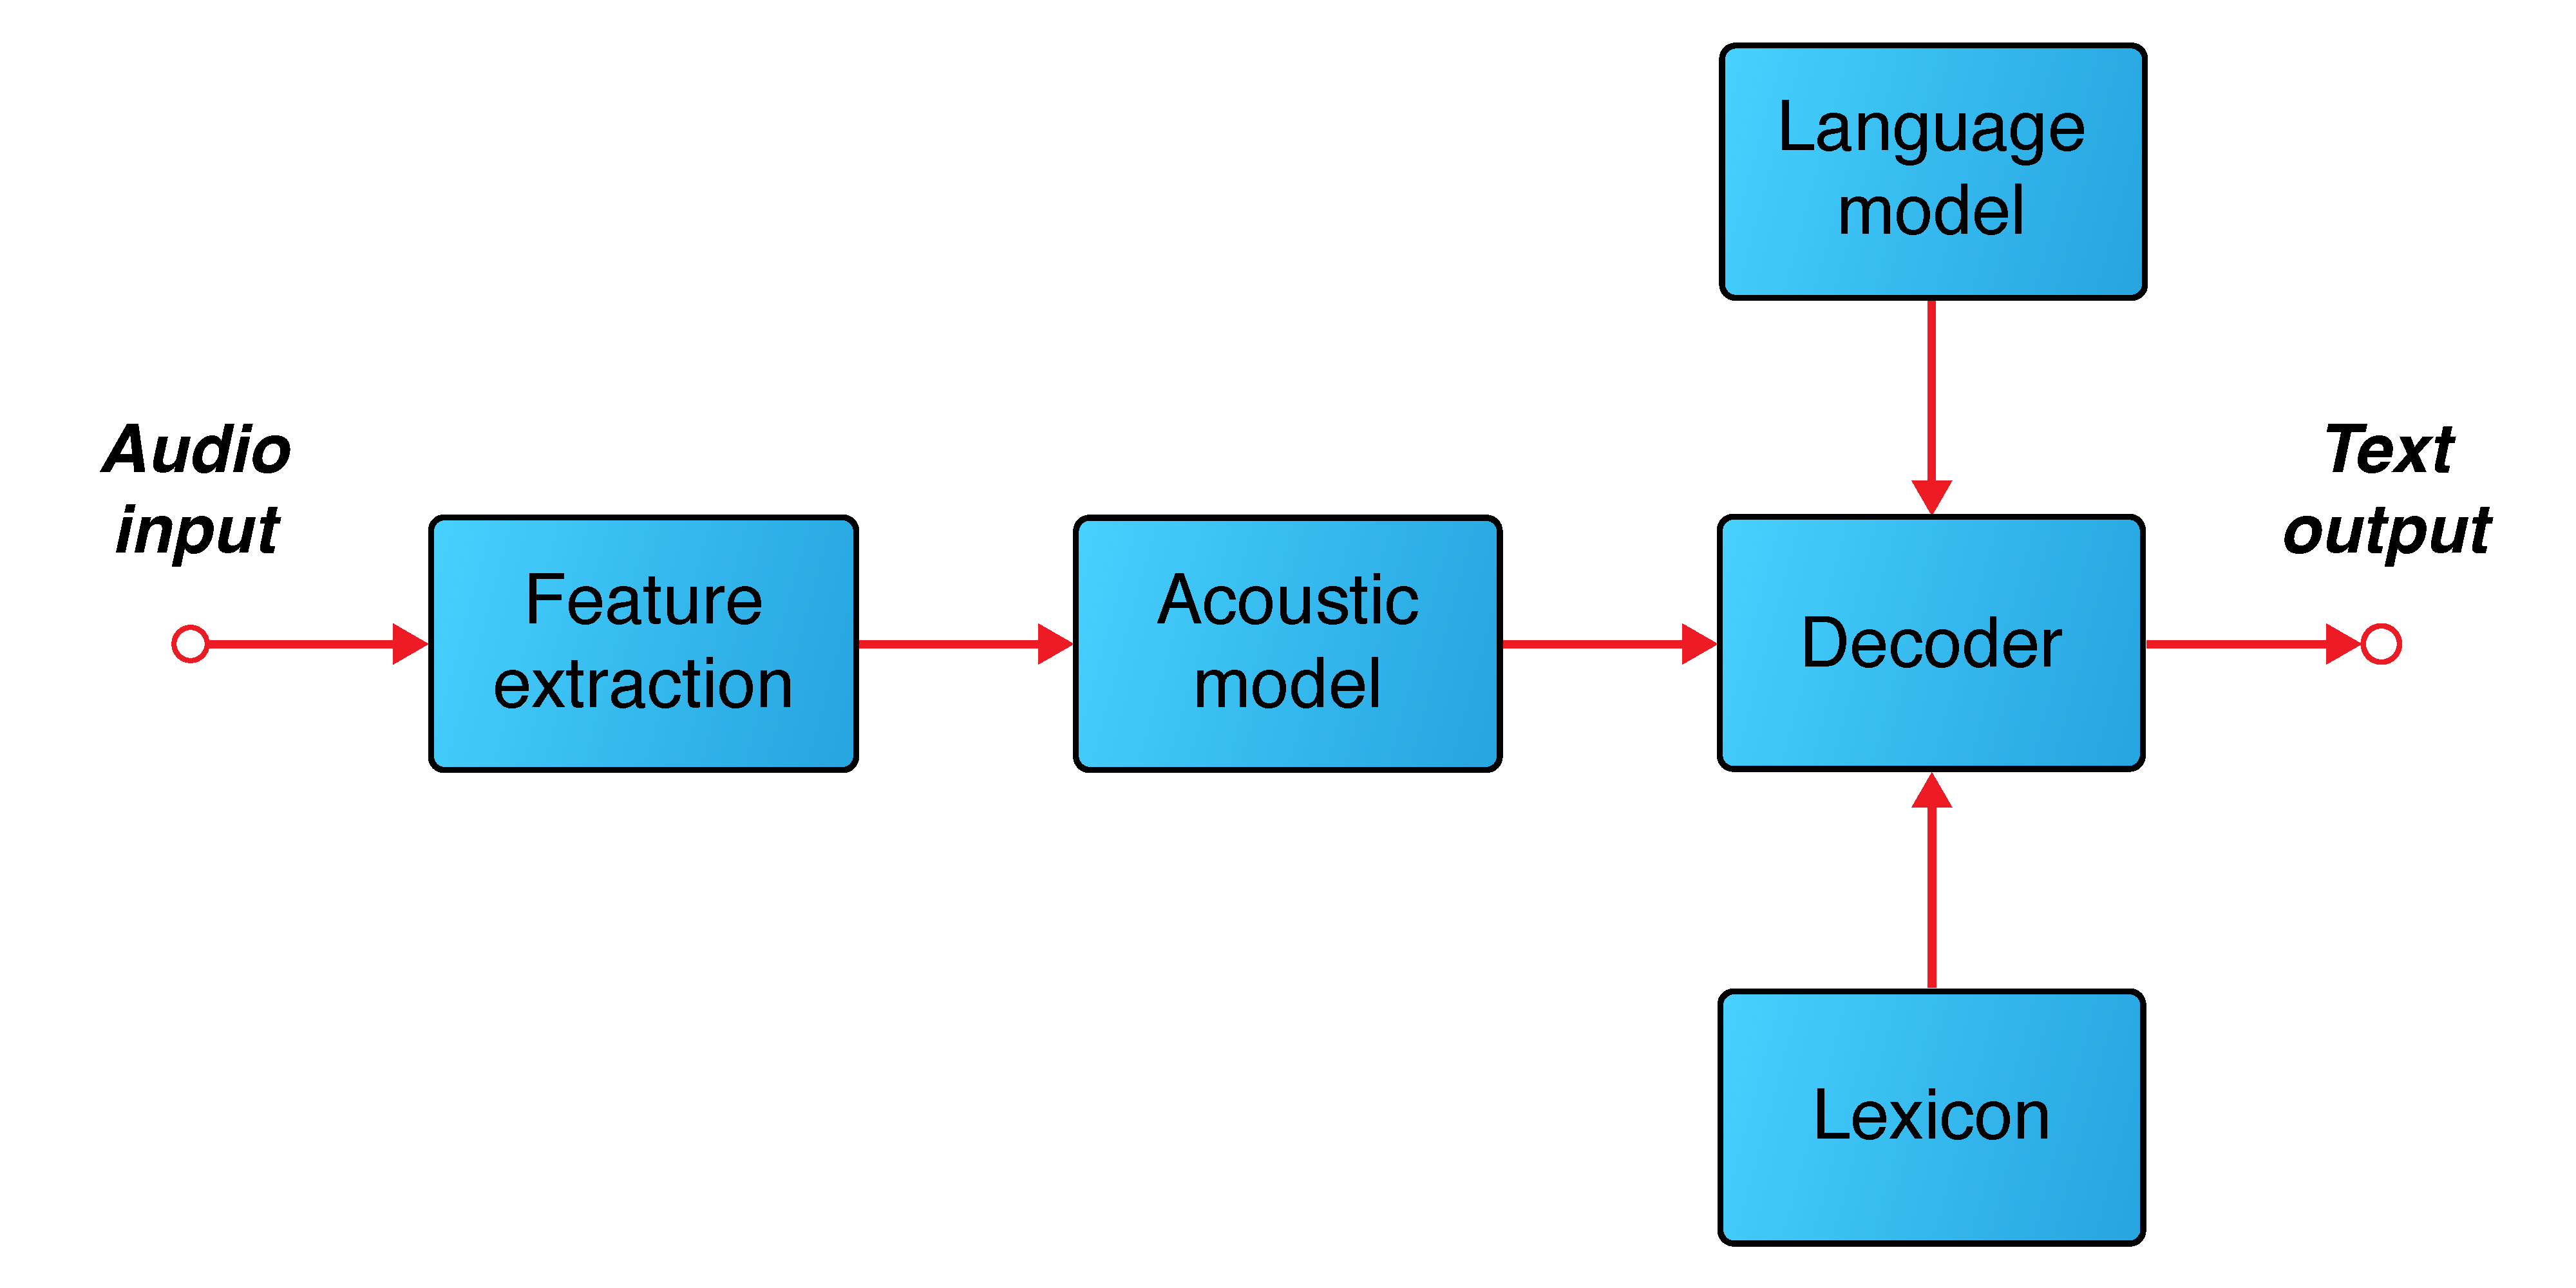
\includegraphics[trim={1.8cm 0cm 1.8cm 0cm}, clip, width=\textwidth]{ASR.pdf}
    \caption{Block diagram for the structure of a typical speech recognition system. The audio input can be a real-time signal from a microphone, or a existing recording or audio track. Depending on the application, the text result can be displayed immediately or saved into a text file.}
    \label{fig:asr} 
\end{figure} \\
At the technical level, automatic speech recognition is a conversion process, where an acoustic data sequence (speech) is converted into a symbolic character sequence (text) \cite{yu2014automatic}. In statistical terms, speech recognition can be categorized as a classification problem among the wider context of general pattern recognition tasks \cite{huang2001spoken}. The speech recognition process can be formulated mathematically in the following way \cite{huang2001spoken, gales2008application, kallasjoki2016}: the goal of the system is to produce the most probable word sequence $ \hat{\bm{W}} = w_1, w_2, w_3,\dots,w_n$, for a given acoustic observation sequence $\bm{O}$. The most probable word sequence corresponding to $\bm{O}$ can be found by maximizing the posterior (i.e., conditional) probability $P(\bm{W} | \bm{O})$:
\begin{equation} \label{eq:max}
\hat{\bm{W}} \ = \ \underset{\bm{W}}{\argmax} \ P(\bm{W} | \bm{O})
\end{equation}
However, $P(\bm{W} | \bm{O})$ is difficult to calculate directly \cite{gales2008application}, but it can be transformed into a form that is easier to model statistically. The Bayes' theorem states that \cite[p.~10]{hori2013speech}:
\begin{equation}
P(A | B) \ = \ \frac{P(B | A) \ P(A)}{P(B)}
\end{equation}
With the Bayes' theorem, the probability $P(\bm{W} | \bm{O})$ can be transformed to the equivalent probability:
\begin{equation} \label{eq:max2}
P(\bm{W} | \bm{O}) \ = \ \frac{P(\bm{O} | \bm{W}) \ P(\bm{W})}{P(\bm{O})}
\end{equation}
For finding the maximum, the denominator in equation (\ref{eq:max2}) can be discarded as it stays constant, and equation (\ref{eq:max}) becomes:
\begin{equation} \label{eq:max3}
\hat{\bm{W}} \ = \ \underset{\bm{W}}{\argmax} \ P(\bm{O} | \bm{W}) \ P(\bm{W})
\end{equation}
Here, $P(\bm{O} | \bm{W})$ is the probability of an acoustic observation sequence for a specific word sequence, corresponding to the acoustic model. $P(\bm{W})$ is the probability of a specific word or word sequence occurring, which is given by the language model. In practice, the probability product is often calculated as an addition in the logarithmic domain, with an additional weight $\alpha$ for controlling how much weight is given to the language model \cite[p.~200]{gales2008application}:
\begin{equation}
\hat{\bm{W}} \ = \ \underset{\bm{W}}{\argmax} \big\{ \log P(\bm{O} | \bm{W}) \ + \ \alpha \log P(\bm{W}) \big\}
\end{equation} \\
The following subsections present a brief review of each individual part of the speech recognition process presented in figure \ref{fig:asr}. In other words, how producing an answer to equation (\ref{eq:max3}) is implemented in practice.

\subsubsection{Feature extraction}

The input to an ASR system is a digital audio signal, the digitized version of an acoustic sound wave and comprised of discrete samples \cite{yu2014automatic, huang2001spoken}. Figure \ref{fig:audio} presents the waveform and the spectrogram for a short speech sample. The spectrogram is the magnitude spectrum of a signal as a function of time, describing how the frequency contents vary temporally.
\begin{figure}[t]
    \centering
    \begin{subfigure}[b]{\textwidth}
        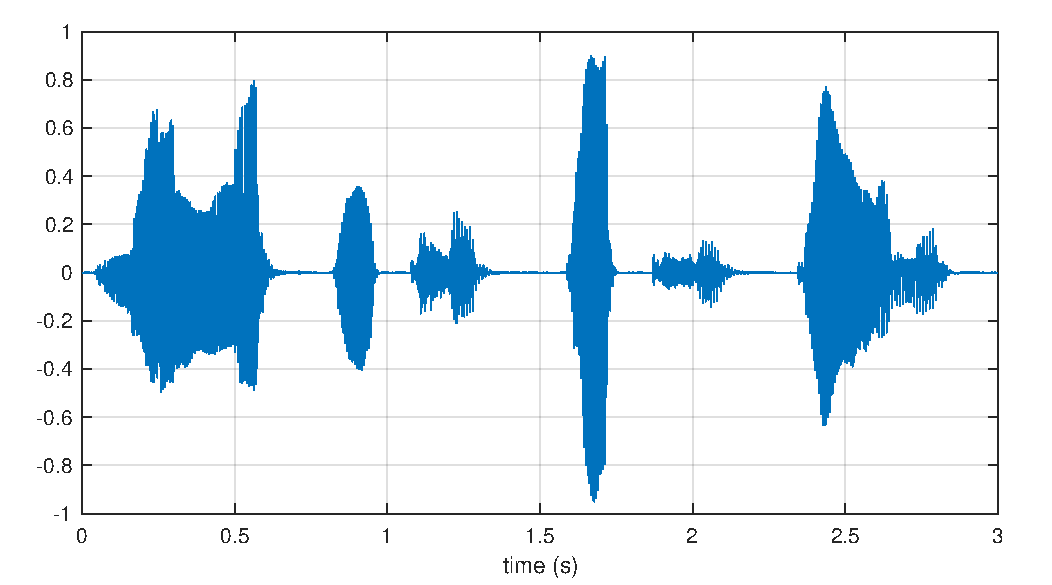
\includegraphics[trim={0.4cm 0cm 0.1cm 0.2cm}, clip, width=\textwidth]{waveform.pdf}
    \end{subfigure}
    \begin{subfigure}[b]{\textwidth}
        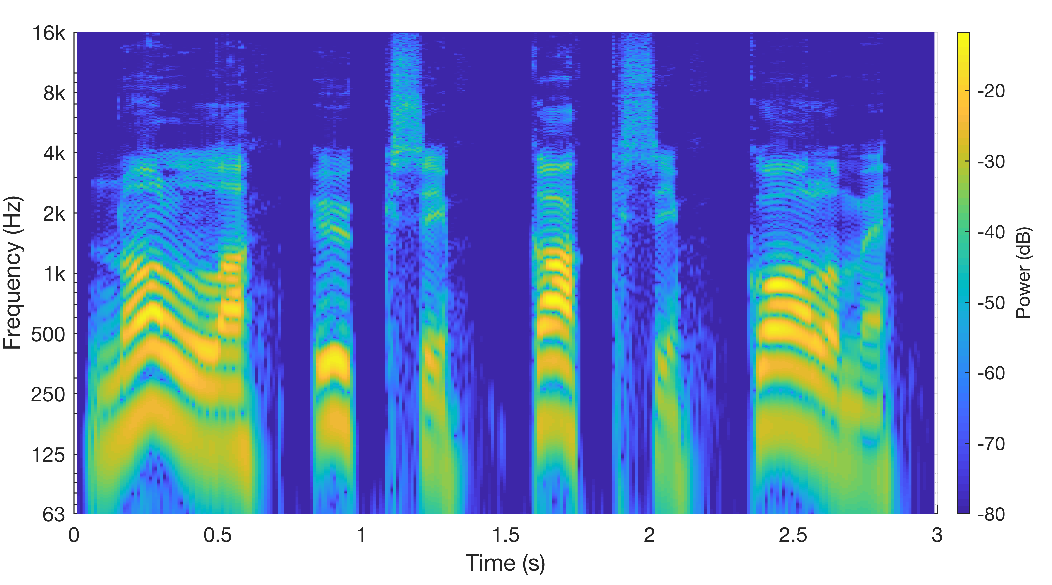
\includegraphics[trim={0.4cm 0cm 0.1cm 0cm}, clip, width=\textwidth]{spectrogram.pdf}
    \end{subfigure}
    \caption{The waveform and corresponding spectrogram of a speech signal containing the words "zero, one, two, three" pronounced in Finnish.}
    \label{fig:audio} 
\end{figure} 
An audio signal contains acoustic information, such as the energy and frequency of its components. But in speech recognition, the interest is in the linguistic information. Therefore, the acoustic properties of an audio sample need to be somehow mapped to linguistic information. However, the problem with recognizing speech sounds is that every person has an unique voice, meaning that the same word or sentence spoken by different persons produce widely varying acoustic information contents. These depend for example on the speakers gender, accent, intonation, tone of voice, mood, and characteristic pitch and timbre. The voice of a one specific individual does not stay constant either, and can vary noticeably between different times and situations. Also, in addition to the speech signal of interest, all real-world signals contain some degree of background noise and other unwanted sounds from the recording environment \cite{huang2001spoken}. Therefore, the acoustic properties of a speech sample cannot be used directly for accurate recognition. \\\\
What is needed are some characteristic measures, or \textit{features}, that can describe and discriminate between different speech sounds, and extract the linguistic information independent of a speaker's personal voice. These features should contain the essential information and measurements needed for classifying speech. \textit{Feature extraction} is then the process of calculating a sequence of these features, a \textit{feature vector}, based on the input audio signal. Ideally, a feature vector should be compact, containing only the necessary information, be robust against noise, as well as fast to calculate so that it can be used in real-time \cite{huang2001spoken}. Consequently, audio signals typically contain a lot of information that is not useful for the recognition task. In feature extraction, the input signal is therefore processed to remove unwanted and redundant information, as well as background noise, while emphasizing the important characteristics for speech recognition. \\\\
Common preprocessing steps include filtering the signal: The very low and high frequencies can generally be removed as speech is mostly focused between the frequencies from 100 to 4000 Hz, as can be seen in the spectrogram in figure \ref{fig:audio}. The input is often downsampled to a lower sampling rate, effectively removing unnecessary high frequencies as all frequencies above the Nyquist limit are lost. In practice, sampling rates as low as 8 kHz can be used, limiting the highest possible frequency to just 4 kHz, without a noticeably reduced recognition accuracy \cite{huang2001spoken}. A pre-emphasis filter can be used to adjust the spectral tilt \cite{kallasjoki2016}. The signal is divided into partially overlapping frames, typically around 20 to 30 milliseconds in length, meaning the frequency content of each frame can be expected to be fairly stationary \cite{huang2001spoken, gales2008application}. \\\\
\textit{Mel-frequency cepstral coefficients} (MFCC) has been a very popular choice for the feature representation type \cite{yu2014automatic, gales2008application, kallasjoki2016}. MFCCs are used for their capacity for eliminating the speaker dependent characteristics of speech, while matching well to the logarithmic loudness and pitch perception of humans. The mel scale (short for \textit{melody}) is a psychoacoustic frequency scale, where the change in pitch is judged to be perceptually equal in distance on the scale \cite[p.~174]{pulkki2015communication}. Compared to the objective frequency scale in hertz, the mel scale puts more emphasis on low frequencies below one kilohertz, and conversely, compresses higher frequencies as the interval between perceptually equal pitch increments starts to increase exponentially with the frequency in hertz. The mel scale is used in order to better match the non-linear properties of human hearing, accentuating the frequency bands that are more important for human auditory perception. A common formula for converting a frequency in hertz to the mel scale is:
\begin{equation} \label{eq:mel}
m \ = \ 2595 \  \cdot \ \log_{10} \ \left(1 \ + \ \frac{f}{700} \right),
\end{equation} where $f$ is the frequency in Hertz. The anchor point where the to scales match is set to 1000 Hz $\leftrightarrow$ 1000 mel \cite[p.~174--175]{pulkki2015communication}. As we are interested in the frequency contents of the signal, each frame is windowed and converted to the frequency domain by calculating the short-time power spectrum \cite{gales2008application}. A mel-scale filter bank with triangular band-pass filters spaced in perceptually equally long frequency bands is applied to each frame. A mel-scale filter bank is presented in figure \ref{fig:melbank}. The combined energy of each frequency band is then calculated. Finally, the cepstral coefficients are obtained by first taking the logarithm of each energy band, mimicking the logarithmic loudness perception of hearing, and applying the \textit{discrete cosine transform}, in effect compressing and decorrelating the energies \cite{huang2001spoken, gales2008application}. The cepstrum can be viewed as the spectrum of a spectrum, since the inverse (discrete) Fourier transform of a log spectrum transforms to the cepstral domain \cite{huang2001spoken}.
\begin{figure}[t]
    \centering
    \includegraphics[trim={0.1cm 0cm 0.1cm 0.5cm}, clip, width=\textwidth]{melfilter_edit.pdf}
    \caption{Mel-scale filter bank with 12 filter bands from 0 to 4000 Hz. Note that in practice the number of filters is typically higher, a low number of filters was used here for a clear illustration.}
    \label{fig:melbank} 
\end{figure}
In essence, the cepstrum operator deconvolves the speech signal into a linear combination of a source (excitation signal) and a filter, which can be then separated \cite[p.~306--307]{huang2001spoken}. In the \textit{source-filter} model of speech production, speech is formed by convolving a speaker-dependent excitation with a speaker-independent formant filter. We want to separate the speaker-independent filter part that corresponds to a specific linguistic unit \cite[p.~288--290]{huang2001spoken}. For an idealized case, this can be represented mathematically in the following way: Speech is modeled as the combination of a sound source (vocal chords) $e(n)$ and an linear acoustic filter (vocal tract) $h(n)$:
\begin{equation}
    s(n) \ = \ e(n) * h(n)
\end{equation}
The Fourier transform converts a convolution in the time domain into multiplication in the frequency domain:
\begin{equation}
    S(k) \ = \ F\big\{ \ e(n) * h(n) \ \big\} \ = \ E(k) \cdot H(k)
\end{equation}
Through the properties of logarithms, multiplication can be separated into addition:
\begin{equation}
    \log S(k) \ = \ \log \big( E(k) \cdot H(k) \big) \ = \ \log E(k) \ + \ \log H(k)
\end{equation}
A linear combination of the source and filter are then obtained with an inverse Fourier transform, which is a linear operation itself:
\begin{equation}
    c(n) \ = \ F^{-1} \big\{ \log E(k) \ + \ \log H(k) \big\} \ = \ F^{-1} \big\{\log  E(k) \big\} \ + \ F^{-1} \big\{\log H(k) \big\}
\end{equation}
In practice, the separation does not work perfectly, as the source-filter model is already a simplification in itself. However, it is often an accurate enough approximation for practical usage \cite[p.~314]{huang2001spoken}. The separation can be done with linear band-pass filtering, referred to as \textit{liftering} in the cepstral domain. In practice, this can be achieved by applying a rectangular window to the cepstrum. Functionally, this is the same as simply dropping the coefficients outside the filter pass-band. Truncating the cepstral coefficients, i.e., taking only the $n$ first coefficients, isolates the speaker-independent filter, meaning the spectral envelope displaying the formants of a speech signal. A traditional number of coefficients used is 12 \cite{huang2001spoken, gales2008application}. Conversely, the higher cepstral coefficients describe the primarily speaker-dependent excitation characteristics, corresponding to the spectral fine structure \cite{gales2008application}. The effect of cepstral truncation on the spectrum is illustrated in figure \ref{fig:cepstrum}.
\begin{figure}[h]
    \centering
    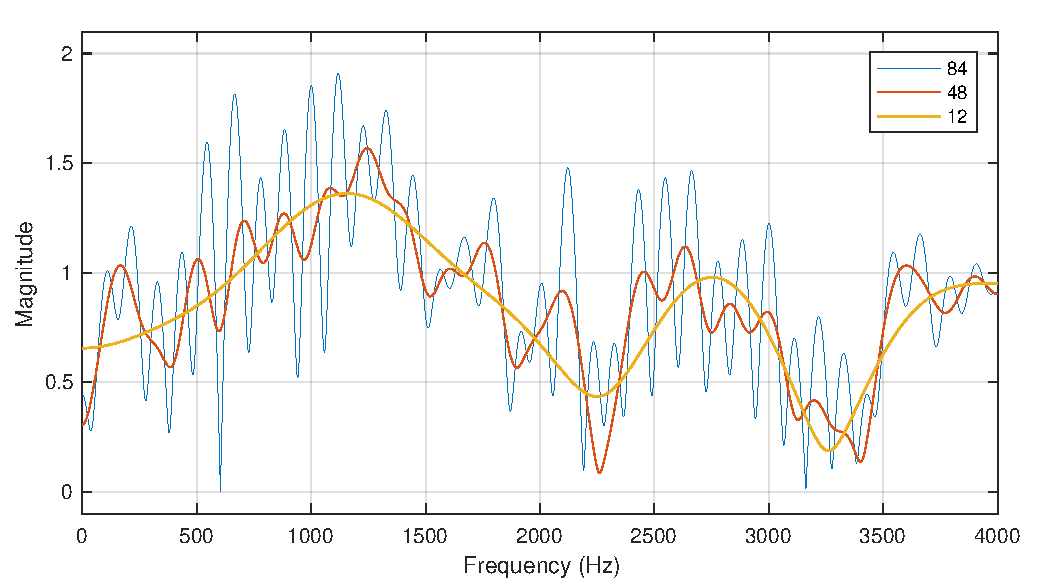
\includegraphics[trim={0.1cm 0cm 0cm 0.4cm}, clip, width=\textwidth]{cepstrum.pdf}
    \caption{The effect of cepstral truncation on the spectrum of a 30ms frame containing the Finnish phoneme $/a/$. The numbers describe how many cepstral coefficients are being used. As the number of coefficients is lowered, the underlying formant structure becomes clear.}
    \label{fig:cepstrum} 
\end{figure} \\
Additionally, the time varying nature of speech can be captured by taking the time derivatives of the obtained cepstral coefficients of consecutive frames \cite{gales2008application, kallasjoki2016}. The first and second-order differences, referred to as the \textit{delta} and \textit{delta-delta} features respectively, are typically used for modeling the dynamic aspects of speech. The end result is a highly condensed set of features \cite{huang2001spoken, gales2008application}. The next step in the automatic speech recognition process is to map the acoustic speech features produced into linguistic classes, which can then be used to form words. This is were the \textit{acoustic model} comes in.

\subsubsection{Acoustic model}

The \textit{acoustic model} provides a statistical model for classifying feature vectors into units of speech \cite{kallasjoki2016}. One of the practical choices for these classes are the \textit{phonemes} of a particular language. Words or longer phrases could technically be used as well, however, this would lead to a very large number of classes as each word or phrase would require its own class. In written language, all words are formed with a very limited set of alphabetic letters, or \textit{graphemes}. In linguistics, a grapheme is the smallest unit of writing in any given language. For example, the English alphabet consists of 26 letters, and in Finnish 29 letters are used. Similarly, phonemes are the different units of sound that can be used to form all possible words in a particular language \cite[p.~24--25]{huang2001spoken}. For example, English is commonly divided into roughly 45 phonemes, varying slightly between different dialects and interpretations. This is very useful for acoustic modeling, since it means the acoustic model needs only to be trained to recognize this small set of phoneme classes, which can then be used to classify a practically unlimited number of different words. As the pronunciation of a phoneme depends quite heavily on the neighboring phonemes, it is common to actually use the \textit{triphone} for the acoustic class. A triphone is a sequence of three phonemes: one phoneme with the two nearest phonemes, meaning the preceding and succeeding phonemes as context. \\\\
\textit{Hidden Markov Models} (HMM) have been widely used for implementing the acoustic model \cite{gales2008application, hori2013speech}. Speech is approximated well by a \textit{Markov chain}, a stochastic model for randomly changing systems where the next state depends only on the current state \cite[p.~23--26]{yu2014automatic}. 
\begin{figure}[b]
    \centering
    \includegraphics[trim={0.1cm 0cm 0.1cm 0cm}, clip, width=\textwidth]{hmm2.pdf}
    \caption{A three-state, left-to-right HMM diagram. $a_{ij}$ is the transition probability from state $s_i$ to state $s_j$. Each state has an emission probability distribution $b_i$ conditional over the observation sequence $O$.}
    \label{fig:hmm} 
\end{figure}
The chain consists of discrete states and state changes that are modeled with transition probabilities. In a hidden Markov model, the states cannot be observed directly (hence the term \textit{"hidden"}). Instead, an output that is dependent on the hidden states is known. In speech recognition, an utterance of a phoneme is considered a hidden state that emits an observable representation in the form of a feature vector. A three-state HMM is generally used to model one triphone in a left-to-right topology, meaning the states are constrained to be in chronological order \cite{kallasjoki2016}. Figure \ref{fig:hmm} present a three-state, left-to-right HMM. The probability that an observation is an emission of a specific state needs to be also modeled. For representing the probability distribution of observations, \textit{Gaussian Mixture Models} (GMM) have been a popular choice \cite{gales2008application, hinton2012deep}. Gaussian mixture models are built by linearly combining two or more multivariate Gaussian distributions together. A simplified example of an GMM is illustrated in figure \ref{fig:gmm}.
\begin{figure}[b]
    \centering
    \includegraphics[trim={0cm 0.2cm 0cm 0.2cm}, clip, width=\textwidth]{gmm2.pdf}
    \caption{A combination of multivariate Gaussian distributions. Note that the scaling is wrong for an actual GMM, as this is only an illustration. A much higher dimensionality is required in reality.}
    \label{fig:gmm} 
\end{figure} \\\\
Like many other aspects in ASR, GMMs have been surpassed by deep neural networks in recent years \cite{hinton2012deep}. A DNN is an artificial neural network that has two or more layers of hidden units between the inputs and outputs. DNNs are typically feed-forward, meaning data flows from the input layer to the output layer without looping back. They are trained with the \textit{backpropagation} algorithm, where the gradient of a cost function measuring the error between the desired and produced output is propagated back to the network layers \cite[p.~57--60]{yu2014automatic}. Significant improvements to speech recognition accuracy have been achieved by replacing GMMs with DNNs \cite{yu2014automatic, hinton2012deep, xiong2016achieving}. The trend of using deep neural networks for acoustic modeling has somewhat affected the way feature extraction is implemented as well, with feature extraction incorporated as one aspect of the acoustic model: The extraction process can be started with a simple linear or mel-scale spectrum, and producing the final feature representation type is relegated to the DNN, meaning the feature representation can be optimized as a part of training the acoustic model \cite{kallasjoki2016}. The ASR system used in this work is DNN based. A detailed description of the models and their training material is given in section \ref{sec:models}.

\subsubsection{Lexicon}

The \textit{lexicon} functions as a bridge between the acoustic model and the language model. It is used to describe how each word in the language model is pronounced by listing the phoneme sequence of every word. In other words, the lexicon can be defined as a dictionary for pronunciation in the context of an ASR system. Single phonemes (monophones) or triphones are normally used depending on the acoustic model. In Finnish, the pronunciation rules are very simple and each phoneme maps directly to one grapheme with only a few exceptions. Therefore, the lexicon can be generated automatically for the most part. For languages with highly irregular pronunciation rules, such as English, the lexicon is more complex and typically needs to be handcrafted by linguistic experts. Different pronunciations for the same word can also be accounted for in the lexicon. Table \ref{table:triphone} presents an example of a triphone lexicon for the same four words in Finnish as in figure \ref{fig:audio}. \\
\begin{table}[h]
    \renewcommand{\arraystretch}{1.2}  % set row height to 1.2x default
    \setlength{\tabcolsep}{20pt}       % set space between text and cell border
    \centering
    \caption{An example of a triphone pronunciation lexicon.}
    \label{table:triphone}
    \begin{tabular}{@{}ll@{}}
        \toprule
        \textbf{Word}  & \textbf{Pronunciation}              \\ \midrule
        nolla & \_--n+o \ n--o+l \ o--l+l \ l--l+a \ l--a+\_ \\
        yksi  & \_--y+k \ y--k+s \ k--s+i \ s--i+\_          \\
        kaksi & \_--k+a \ k--a+k \ a--k+s \ k--s+i \ s--i+\_ \\
        kolme & \_--k+o \ k--o+l \ o--l+m \ l--m+e \ m--e+\_ \\ \bottomrule
    \end{tabular}
\end{table}

\subsubsection{Language model}

The \textit{language model} contains information on how words are used to form meaningful sentences in a particular language. Instead of grammatical rules about what combinations are theoretically possible, the language model tells which words typically go together and how often they are used. Specifically, it gives the likelihood for the occurrence of a specific word sequence, which is estimated from large collections of suitable written text called a \textit{text corpus} \cite{kallasjoki2016}. Thus, the language model can be used to choose the most probable word sequence from multiple similar sounding candidates suggested by the acoustic model. Take for example the words \textit{beer} and \textit{bear}, which sound fairly similar to each other. While the sentence \textit{"one bear please"} is grammatically correct and quite possible, it is typically much more likely that \textit{"one beer please"} was uttered instead. The language model will likely assign a higher probability to the phrase \textit{"one beer please"} (depending obviously on the data it was trained with). This way, verbal context is provided for the recognition task, sorting the different hypotheses according to which are sensible and commonly used. The language model can also be used to efficiently reduce and rule-out unwanted and incorrect sentences, as word sequences with a probability of zero cannot be recognized. \\\\
Mathematically, the language model can be presented in the following way: Let $\bm{W} = w_1, w_2, w_3,\dots,w_n$ be a word sequence. The objective of the language model is to estimate the probability $P(\bm{W}) \ = \ P(w_1, w_2, w_3,\dots,w_n)$, the likelihood of that specific word sequence appearing in a particular language. Applying the chain rule of probability gives:
\begin{equation}
    P(\bm{W}) \ = \ P(w_1) P(w_2|w_1) P(w_3|w_1,w_2) \dots P(w_n|w_1,\dots,w_{n-1})
\end{equation}
This means that the conditional probability $P(w_i|w_1,w_2,\dots,w_{i-1})$ must be estimated for every word $w_i$, which is generally done using \textit{maximum likelihood estimation} \cite{arisoy2008statistical}. The estimate can be calculated as the ratio of the occurrences of the word sequences $w_1,w_2,\dots,w_{i-1},w_i$ and $w_1,w_2,\dots,w_{i-1}$:
\begin{equation} \label{eq:ml}
    P(w_i|w_1,w_2,\dots,w_{i-1}) \ = \ \frac{C(w_1,w_2,\dots,w_{i-1},w_i)}{C(w_1,w_2,\dots,w_{i-1})},
\end{equation}
where $C(\bm{W})$ is the frequency count of a word sequence $\bm{W}$ in a large text corpus. Due to data sparsity, this estimate has traditionally been too unreliable for long word sequences \cite{gales2008application}. As an approximation, a word $w_i$ can be assumed to depend only on a limited number of previous words. This is the \textit{n-gram model}, where the conditional probability is truncated to depend only on the $n-1$ preceding words:
\begin{equation}
    P(w_i|w_1,w_2,\dots,w_{i-1}) \ \approx \ P(w_i|w_{i-n+1},\dots,w_{i-2},w_{i-1}),
\end{equation}
with $n$ ranging typically from two to four \cite[p.~210]{gales2008application}. The n-gram model has been the preferred way to construct language models for a long time \cite{gales2008application, kallasjoki2016, hirsimaki2009importance}. In practice, the n-gram probabilities estimated with equation (\ref{eq:ml}) need to be balanced, since n-grams that are present in the training material tend to get a too high probability and unseen sequences a too low probability. This process is called language model \textit{smoothing}, and can be achieved by distributing some probability mass from seen n-gram combinations to all unseen n-grams \cite{gales2008application}. \\\\
In recent years, \textit{recurrent neural networks} (RNN) have been shown to work well for language modeling \cite{enarvi2017automatic}. Due to the recurrent connections enabling arbitrarily long context information in the network, RNN language models can capture the long-term dependencies ignored by the simple n-gram model \cite{enarvi2017automatic, mansikkaniemi2017continuous}. Neural network language models overcome the data sparsity problem by projecting words into continuous space, where the probabilities are then estimated \cite{mansikkaniemi2017continuous}. While neural network language models offer improved performance for many applications, training them requires a great deal more computational resources compared to n-gram models, with the training time typically measured in days or even weeks on high-end GPUs. Memory consumption of state-of-the-art neural networks can be an issue as well on currently available GPU hardware \cite{enarvi2017automatic}. Also, the recognition speed is typically slow. \\\\
In agglutinative languages like Finnish, Estonian, Hungarian and Turkish, words are formed primarily by concatenating suffixes to root words, as well as using compounding (i.e., joining words together) and inflections (word bending) \cite{arisoy2008statistical, kurimo2006unlimited, hirsimaki2006unlimited}. This means that there can be millions of regularly used word forms in these languages. Therefore, it is very hard to build a word-based vocabulary that would cover all the commonly used words \cite{arisoy2008statistical}. Though it has recently become possible to build n-gram models covering millions of words, reducing the vocabulary size is important for efficient models \cite{smit17boundaries}. For English, a 60 000 word lexicon can be sufficient for many tasks, whereas for Finnish, even a 500 000 word-based lexicon would not give the same level of performance \cite{arisoy2008statistical}. The problem is the large number of \textit{out-of-vocabulary} words when dealing with limited vocabulary sizes. \textit{Sub-word modeling} has been successfully used to model agglutinative languages, reducing the size and complexity of the language model \cite{enarvi2017automatic, hirsimaki2009importance, hirsimaki2006unlimited, smit17boundaries}. In sub-word modeling, words are split into smaller units, which can be done based on grammatical rules or statistical techniques \cite{arisoy2008statistical}. A data-driven statistical method called the \textit{Morfessor} is commonly used for morphological segmentation. The Morfessor uses unsupervised machine learning methods to find morpheme-like statistical sub-word units called \textit{morphs}, based purely on raw text data \cite{arisoy2008statistical, kurimo2006unlimited}. A morph-based vocabulary was used in the Conversation Assistant prototype, since it uses Finnish speech recognition.

\subsubsection{Decoding} \label{sec:decoding}

In ASR systems, \textit{decoding} means computing the result based on the input and the statistical models, i.e., solving equation (\ref{eq:max3}), were the observation sequence $\bm{O}$ is the feature vector produced in feature extraction. The decoding process is fundamentally a search for the best matching word sequence over all possible word sequences, i.e., the \textit{search space} defined by the models \cite{pylkkonen2013towards}. However, implementing the search in practice requires efficient algorithmic solutions: The size of the search space is often huge, and grows exponentially with the number of words in an utterance \cite{pylkkonen2013towards}. Therefore, an exhaustive search over all possibilities is generally not feasible. Heuristic methods are required to limit the search space in some way. For this purpose, \textit{beam search} is commonly used \cite{pylkkonen2013towards, hori2013speech}. In beam search, only a limited number of most promising paths are kept while others are discarded in a process called \textit{pruning}. The \textit{Viterbi} dynamic programming algorithm is one such commonly used method \cite{huang2001spoken, yu2014automatic, hori2013speech}. \\\\
ASR systems are divided into \textit{online} and \textit{offline} decoders \cite{alumae2014full}. In online decoding, the input is coming continuously in real-time and speech recognition is performed concurrently with the input. In other words, speech recognition is performed in real-time and the results are typically displayed immediately. Conversely, in offline decoding the input is an existing (long) audio recording, which is then transcribed into text all at once. Offline decoding generally focuses on accuracy at the cost of speed and model size, though offline decoding can also be faster than real-time, meaning that the full transcription result is produced in less time than the length of the input file \cite{alumae2014recent}. For example, a ten minute audio file could be transcribed in five minutes. On the other contrary, online decoding sets some restrictions for the properties of the ASR system, with the primary constraint being the requirement of approximately real-time recognition. Therefore, a compromise between speed and accuracy is typically required in online recognition. For example, the size of the vocabulary may have to be limited for fast enough performance \cite{mcgraw2016personalized, enarvi2017automatic}. \\\\
The use of \textit{weighted finite-state transducers} (WFST) for representing the statistical models is popular in speech recognition, especially for LVCSR systems \cite{hori2013speech, mohri2008speech, smit17boundaries}. WFSTs can be understood as a finite automaton, consisting of a set of finite states and transitions between them. Each transition has an input label, output label and a weight for the transition. They are typically used to represent and store the acoustic model, language model and lexicon in one combined transducer, which offers many practical benefits. In the WFST--based speech recognition process, the acoustic model WFST transduces an acoustic state sequence into a phoneme sequence, the lexicon WFST transduces a phoneme sequence into a word sequence, and the language model WFST transduces a word sequence into a sentence. These transducers can be integrated into a single, large WFST that directly transduces an acoustic state sequence into a sentence. The power of weighted finite-state transducers for ASR comes from that they can optimize the search space and remove redundancies. The end result is a highly-optimized static structure for fast decoding, enabling real-time decoding with very large vocabularies of over one million words even on an average personal computer \cite[p.~4--6]{hori2013speech}. However, the memory requirements for WFSTs can be large due to the fully expanded static search network, instead of it being dynamically created during decoding. The ASR system used in the Conversation Assistant prototype is a WFST-based online decoder, described in detail in section \ref{sec:kaldi}.

\subsubsection{Evaluation metrics}

Measuring the performance of an ASR system is a critical part of their development, so that different systems can be compared and new algorithms or implementations evaluated \cite{huang2001spoken}. However, the answer to the question of how to measure speech recognition errors is not wholly unambiguous. It depends on what kind of occurrences in the transcription are defined as errors: For instance, are missing punctuation marks or capital letters counted as errors. In the recognized word sequence, there might be extra words added to the result or some words could be missing, in addition to the simple recognition errors were a word was transcribed incorrectly. Consequently, simply comparing two word strings one word at a time does not work: For example, if one word is missing or added as an extra, all the following words are interpreted as errors since they do not match the reference word in that position of the sequence. Instead, the recognition result and the reference word sequence have to be aligned to each other \cite{huang2001spoken}. Typically, the recognition errors in an ASR system are categorized as one of three main types of errors \cite[p.~420]{huang2001spoken}:
\vspace{2mm}
\begin{itemize}[itemsep=2mm]
    \item \textbf{Substitution}: a correct word was replaced with an incorrect word.
    \item \textbf{Deletion}: a correct word was omitted.
    \item \textbf{Insertion}: an extra word was added.
\end{itemize} 
\vspace{2mm}
Based on these, the \textit{word error rate} (WER) is defined as:
\begin{equation}
WER \ = \ \frac{S + D + I}{N} \cdot 100\%,
\end{equation}
where $S$ is the number of substitutions, $D$ is the number of deletions, $I$ is the number of insertions and $N$ is the total number of words in the reference text. Essentially, it is the \textit{Levenshtein distance} for words, describing the total percentage of word errors. It should be noted that it is possible for the error rate to exceed $100\%$, as the number of insertions is not limited. WER is the most widely used metric for evaluating and comparing the speech recognition accuracy of ASR systems \cite{huang2001spoken, kallasjoki2016}. For agglutinative languages such as Finnish, the WER can be a too harsh measure: Many words are formed by adding affixes to a base word, resulting in a large amount of very similar sounding words with only a slight difference in their meaning. While technically incorrect, recognition errors of one or two characters in these words will most likely not hinder the understandability as much as the WER indicates. The \textit{letter error rate} (LER) can be used as an alternative to the WER, giving a more accurate metric for agglutinative languages \cite[p.~41--42]{kallasjoki2016}. In LER, the Levenshtein distance is simply calculated for individual letters instead of full words. Other measures can be used as well, particularly for measuring very specific types of errors or special vocabulary words, such as the error rate of foreign names or acronyms \cite{mansikkaniemi2017continuous}. Suitable text error measures for the Conversation Assistant are discussed in section \ref{sec:loppu}. \\\\
For evaluating language models, the \textit{perplexity} measure is commonly used \cite{mansikkaniemi2017continuous}. Perplexity measures how accurately a statistical model predicts a sample. In the case of the language model, this translates to how well the language model predicts a word sequence in an evaluation text sample. Perplexity is calculated by
\begin{equation}
    ppl \ = \ \sqrt[N]{\prod_{i=1}^{N} \frac{1}{P(w_i|h)}},
\end{equation}
where $P(w_i|h)$ is the probability of a word sequence given by the language model and $N$ the number of words in the evaluation text. Minimizing perplexity corresponds to maximizing probability, meaning that a lower perplexity value is better \cite{mansikkaniemi2017continuous}.

\subsubsection{Recognizing conversational speech} \label{sec:lvcsr}

Accurate speech recognition of everyday conversational speech has been the focus of much research in recent years, and remains challenging especially in noisy environments \cite{keronen2014approaching, kallasjoki2016, xiong2016achieving, li2014overview, keronen2010comparison, pylkkonen2013towards}. This particular area of ASR is the most relevant in the context of this work, as the Conversation Assistant is intended for use in everyday conversational situations. Conversational speech falls under the large vocabulary continuous speech recognition task, and is arguably the hardest area for online ASR. Conversational, or \textit{colloquial} speech, is typically quite informal and can differ noticeably from the standard, formal form of the language \cite{enarvi2017automatic}. In Finnish, colloquial pronunciations are also written differently than the standard word form, due to the phonetic orthography \cite{enarvi2017automatic}. Consequently, colloquial speech causes more variations to language and increases the size of the vocabulary. For agglutinative languages, a vocabulary of many million words is required in order to cover all the spelling variations in conversational speech \cite{enarvi2017automatic}. Overall, these factors have made it significantly harder to achieve a good level of speech recognition performance for conversational speech, compared to most other tasks. \\\\
Different dialects and pronunciations can pose a challenge to ASR performance, as the statistical models are only as good as the material they are trained with. Neural networks require a large amount of training data, and sourcing suitable training data covering the wide variety of distinct speaking styles can be difficult \cite{mansikka17parliament}. In order to recognize colloquial variations such as heavy accents, tens or hundreds of hours of material is typically needed for good performance. In addition, the recordings have to be accurately transcribed and aligned correctly. Even if recording are available, transcriptions are typically not, and producing them is generally expensive and time consuming \cite{mansikka17parliament}.  \\\\
Conversations are often held in acoustically challenging situations with background noise and other competing speakers. For large-scale everyday usage of ASR, noise-robustness has become an integral part for good real-world recognition performance \cite{li2014overview}. More specialized ASR tasks can be performed in a quiet environment and with special, studio-grade microphone equipment, conforming to the limitations of the ASR system. For public usage, ASR systems have to cope with all possible environments and situations instead. Likewise, external microphone setups that could noticeably improve the SNR of the input signal are an unreasonable requirement for most everyday usage. Noise-robust speech recognition remains somewhat a challenge, though a large amount of research has been done to address this issue \cite{keronen2014approaching, li2014overview, kallasjoki2016, keronen2010comparison, qian2016very}. Fundamentally, the problem arises from distortions in the transmission path of the signal from the speaker to the microphone, with the effect that the observed feature sequence does not match the utterance of the speaker \cite{li2014overview, kallasjoki2016}. These distortions can be from sources such as traffic noise, reverberation, background music, and overlapping speech. \textit{Noise-robust} speech recognition methods attempt to reduce the mismatch between the noisy observations and the models \cite{li2014overview, kallasjoki2016, keronen2010comparison}. One straightforward way to improve speech recognition in noisy conditions is to use \textit{multi-condition training}, where the acoustic model is trained with a combination of clean and noisy data. The feature extraction process can be improved further from the standard MFCC features to be more robust against noise. Additionally, \textit{feature enhancement} methods have been presented that adaptively compensate for distortions in the features, such as using imputation methods for reconstructing missing data. Besides training noise robust models, the model parameters can adapted in real-time to the prevailing conditions \cite{kallasjoki2016}.

\subsection{Software Engineering} \label{subsec:soft}

This section reviews briefly the software engineering principles and development methods relevant to this work. The focus is primarily on user-centered design and related user testing methods, which together form the background framework for developing and validating the Conversation Assistant successfully. The concept of \textit{usability} forms the basis of the user-centered design philosophy \cite{richter2014user, deuff2013user}. Usability is defined in section \ref{sec:usability}. Section \ref{sec:user} describes the user-centered design approach, providing an explanation and rationale for the usage of this particular development philosophy for realizing the Conversation Assistant. Section \ref{sec:usertesting} focuses on testing and evaluating usability in practice, a process that is referred to as \textit{usability testing}. Usability testing is tightly connected to the user-centered design process, forming one of the key activities in it \cite{rubin2008handbook}. The most relevant topic in the context of this work is the planning and organization of user tests. Topics such as user interface design and other usability evaluation methods are left outside this review.

\subsubsection{Usability} \label{sec:usability}

The concept of usability is essential in the user-centered design philosophy. Usability is sometimes used only in a narrow sense to refer to the quality of an user interface design, but usability should be viewed as much more than that \cite[p.~3]{richter2014user}: The usability of a system should be assessed in the context of its use to, and is used to measure how well the users can achieve the tasks they wish to perform. Good usability means that the users learn to use the software easily, the usage is effective, and they can achieve their intended objectives satisfactorily. The ISO 9241-11 standard defines usability as \textit{"the extent to which a product can be used by specified users to achieve specified goals with effectiveness, efficiency and satisfaction in a specified context of use"} \cite[p.~4]{richter2014user}. \\\\
However, usability should not be considered purely from a functional and objective viewpoint \cite{richter2014user, riihiaho2015}. The \textit{user experience} relating to the user's perceptions and feelings of using a software product or system should be taken into account as well \cite[p.~5--6]{richter2014user}. Hearing impaired individuals, particularly the deaf, form a distinct user group that can have very different needs and abilities compared to most other users \cite{potter2014design, korte2015experience}. These subtle differences in the \textit{human-computer interaction} (HCI) have to be accounted for when designing software and user interfaces specifically for these individuals, in order to make it accessible and usable \cite{savidis2004unified}. Consequently, usability can be divided into the following subcategories \cite[p.~4--5]{rubin2008handbook}: 
\begin{multicols}{3}
    \centering
    \begin{itemize}[leftmargin=1.2cm, itemsep=2mm]
        \item Usefulness
        \item Efficiency
        \item Effectiveness
        \item Learnability
        \item Satisfaction
        \item Accessibility \\
    \end{itemize}
\end{multicols} %\vspace{1mm}
\noindent 
Usefulness means the degree to which a product enables the users to achieve their goals, and is an assessment of the user's willingness to use the product. Efficiency means how quickly and accurately the user's goals can be achieved. Effectiveness refers to the product working like the user expects, and how easily the user can do what they intend. Learnability refers to the user's ability to learn to use the system, relating closely to effectiveness. Satisfaction refers to the user's perceptions and feelings towards using the product. Accessibility means making the product usable for people with disabilities, which usually has the added benefit of improving it for all others as well.

\subsubsection{User-centered design} \label{sec:user}

User-centered design can be understood as the methods and techniques for attaining high usability and an excellent overall user experience \cite{richter2014user, deuff2013user}. The user-centered philosophy emphasizes the user as the center of focus in the design and development process, meaning that these activities are based on the needs of the real-world users. The approach is generally considered to have been pioneered in the book \textit{Usability Engineering} by Jakob Nielsen, published in 1993 \cite{richter2014user, nielsen1993usability}. The reason for needing this type of methodology can be summarized with the sentence: \textit{"the developer is not the user"}. In essence, this illustrates the fact that the developers and intended users can have very different viewpoints and skills when using the system \cite{richter2014user, deuff2013user}. As such, a software or system should be optimized for how the users can and want to interact with it, instead of the users having to adapt to the way a developer thinks, or worse, the way a developer imagines the users to think. \\\\
Developers are typically experts who have specialized and been immersed in the relevant technology for a long time \cite[p.~2]{richter2014user}. Therefore, it can be hard for a developer to think like an unskilled user would, meaning that many of the assumptions made in the design might not match very well to how the actual users experience them. Especially in the case of designing and developing the Conversation Assistant, the target user group consists of hearing impaired individuals that have inherently different perspectives and ways to experience the world compared to a normally hearing person. User-centered design is therefore needed to systematically include the perspective of the user in the whole development process \cite{richter2014user, deuff2013user, nielsen1993usability}. Though the focus in this work is on software development, designing products user first is an universal approach. In the wider context, the same principles and philosophy can be applied to many other engineering fields as well in the form of user-centered engineering \cite{richter2014user}. In practice, the user-centered design and development process is generally comprised of the following steps \cite[p.~11--16]{richter2014user}:
\begin{enumerate}[itemsep=2.2mm]
    \item \textit{Analysis:} \\ Identifying and understanding the intended users, their needs and the context of usage.
    \item \textit{Requirements:} \\ Specifying the requirements for the product based on the analysis.
    \item \textit{Realization:} \\ Designing and developing a solution meeting the requirements.
    \item \textit{Evaluation:} \\ Evaluating the produced solution from the user's perspective.
    \item \textit{Iteration:} \\ Refine the requirements and design based on the evaluation and user feedback.
\end{enumerate}
\vspace{1mm}
In short, a requirement is generally a single functional need that the system must perform or fulfill. These can be modeled for instance with \textit{use cases} and \textit{user stories} \cite{richter2014user}. For the realization, these specifications need to be transformed into a technical design and software architecture for practical implementation. User evaluation and iterative development are the key concepts in the user-centered process for guiding the development towards increasing usability and value for the users. Figure \ref{fig:iteration} illustrates the design iteration process. 
\begin{figure}[b]
    \centering
    \includegraphics[trim={0cm 0cm 0cm 0.2cm}, clip, width=0.84\textwidth]{iteration.pdf}
    \caption{The design iteration cycle. Requirements are turned into a prototype implementation. The prototype is evaluated to measure if and how well the goals are met. Requirements and the resulting design are then adjusted accordingly. This cycle can be continued as long as desired or necessary.}
    \label{fig:iteration} 
\end{figure}
The idea of an iterative process matches well to modern agile software development methods, were iterations and prototypes are produced in short cycles with feedback incorporated after each cycle \cite[p.~5--8]{deuff2013user}. Evaluation can be performed for example with formal and informal usability testing methods, cognitive walkthroughs and expert reviews \cite[p.~24]{richter2014user}.

\subsubsection{Usability testing} \label{sec:usertesting}

The term \textit{usability testing} can be defined as using \textit{user testing} for the purpose of \textit{usability evaluation}. In other words, usability testing is a user testing method where one or more intended users perform tasks under observation \cite{riihiaho2015}. It is an empirical method for gathering data for the purpose of improving the software product being tested \cite{dumas1999}. However, not all user testing is necessarily usability testing \cite{de2009usability}. Validating the Conversation Assistant approach is closely related to the usefulness component of usability. Usability testing has become the standard way to test and evaluate software with users, and as such, has been comprehensively researched and written about in scientific literature \cite{deuff2013user, rubin2008handbook, riihiaho2015}. \\\\
The usability testing process has three main phases: design and preparation of the user test, conducting the test sessions, and analysing the results \cite{riihiaho2015}. The test situation is comprised of predefined tasks that the test users need to perform in the test session. These tasks correspond to a particular use scenario or functionality of the software. Particularly for functionally rich and complex products, everything cannot be tested simultaneously \cite{dumas1999}. Therefore, the tasks are chosen based on the goals for the testing, i.e., what particular area or feature is being investigated. There are basic guidelines that need to be adhered to for valid and successful usability testing results: The tasks should remain standard, meaning they are the same for each participant \cite{richter2014user}. Also, the tasks should be performed under the same conditions to enable reliable data gathering \cite{riihiaho2015}. The quality of the results depends in large part on how the tasks are designed and prepared. A common principle for formulating the tasks is that they should represent a realistic scenario from the user’s point of view \cite[p.~62]{richter2014user}. The test participants should be drawn from the intended user group for the application, meaning they should be individuals who may or will use the system in practice \cite{riihiaho2015}. Friends, family members or co-workers should generally be avoided in user testing, as the close relationship can easily bias the results \cite[p.~32]{riihiaho2015}. \\\\
For gathering data, many different methods can be employed \cite{rubin2008handbook, ebling2000contributions}. The test situation is commonly recorded from one or more viewpoints. Likewise, the user's inputs and the output of the software can be recorded. Key logging is one such potential method. The time and steps taken to complete a task, or the number of errors made in an attempt, can be measured for quantitative data collection \cite{ebling2000contributions}. Questionnaires and surveys are commonly utilized for collecting background information and feedback. Questionnaires are the primary way to elicit the opinions of the test users, and can also be used to collect numerical data for statistical analysis \cite{rubin2008handbook}. Research into the relative value of different forms of empirical data in usability testing suggests that verbal feedback is the major source of evidence for usability problems \cite{ebling2000contributions}. The particular methods that should be used depend heavily on the product being tested and the goals of the testing. The amount of test users needed also depends on many factors, such as what is being tested and how formal the testing is. Quantitative testing using a large number of test participants is typically unnecessary for finding critical usability issues: Five participants is commonly cited as the number needed for already discovering 80\% of usability problems \cite{rubin2008handbook, riihiaho2015}. Overall, user testing does have some fundamental limitations \cite[p.~26]{rubin2008handbook}: The testing situation is always artificial and controlled, even if testing in the field. Of course, a software product can be given to test users to use on their own time with feedback then gather from them, but this is different from the formal user testing methods described here. The participants are also rarely fully representative of the whole target user group.

\subsection{Previous Work} \label{subsec:work}

In this section, previous approaches to solve the communication problems of the hearing impaired are reviewed. The main focus of this review is on research into the application of automatic speech recognition technology for alleviating these problems. The idea of using speech recognition technology to support the deaf and hard of hearing is not new to this work. The idea of using speech recognition as an assistive technology for the deaf and hard of hearing dates back to at least 1996 \cite{robison1996computer}. Karjalainen et al. investigated the feasibility of this type of approach using Finnish phoneme-based speech recognition already in the year 1997 \cite{karjalainen1997applications}. While ASR technology has improved greatly in the recent years \cite{yu2014automatic}, previous research can still offer insights and historical perspective for the development of the Conversation Assistant. \\\\
One common focus in previous research has been for supporting the education and inclusion of hearing impaired students in schools and classrooms by providing transcriptions of speech \cite{kheir2007inclusion, stewart2003application, fen2010using, jun2010exploration, jimenez2011tablet, ranchal2013using, kawas2016improving}. Stewart and McKee investigated using speech recognition technology in practice to support deaf higher education students in lectures already in 2003 \cite{stewart2003application}. Their students relied primarily on sign language interpreters, which caused many practical problems. Firstly, the availability of sign language interpreters was problematic, as in many cases they had to be booked months in advance. Even when interpreters were available, the problem they encountered in the higher education setting was that interpreters had major difficulties translating complex technical and scientific vocabulary. As an example of this, the authors give the phrase "isochronous data transmission over Firewire or as it is also known, IEEE1394", which an interpreter could not translate at all. Furthermore, the international student body caused additional complications, as the sign languages used by people from different countries are not identical. For example, the British Sign Language and the American Sign Language differ quite significantly, even though both nations use English in verbal communication. As a solution, the authors tried using a commercial speech recognizer (IBM Via Voice), which was reportedly considered the best commercially available continuous speech recognizer at the time. They found that while the concept was valid, deaf students liked the approach, and that it could improve the comprehensibility of a lecture, in general, speech recognition technology was not ready for the challenge. \\\\
Other previous proposals for ASR-based assistive applications for communication include the following: In 2006, Matthews et al. presented a mobile sound transcription tool using offline speech and acoustic event recognition  \cite{matthews2006scribe4me}. When the user pressed a button in the application, the last 30 seconds of sound were uploaded to a server for transcription, and send back as a text message. The message included dialog and descriptions of environmental sounds. Gelder et al. described a transcription table design, a table prototype with integrated displays for each person for providing text support during meetings \cite{van2005transcription}. Transcriptions are provided for each person around the table in order not to stigmatize hearing impaired meeting participants. Lee et al. described a mobile conversational assistance system that uses acoustic beamforming with a multi-channel microphone array for suppressing background noise \cite{lee2013dialogue}. The beamforming array is used to pick up sound from the direction of the speaker, while attenuating sound from other directions. \\\\
Mirzaie et al. used the \textit{audio-visual speech recognition} (AVSR) technique for speech-to-text translation for deaf and hard of hearing people \cite{mirzaei2012combining}. The results were displayed utilizing \textit {augmented reality} (AR), where the text was displayed floating next to the speaker on a screen. The AVSR system combines audio-based speech recognition with computer vision detection of the mouth and facial expressions of the speaker. A visual feature observation set is produced from consecutive video frames of the tracked mouth region of the speaker. The audio and video features are processed jointly to produce the speech recognition result. Adding the vision-based component can help the recognition accuracy especially in noisy situations. However, the AVSR system used was an offline recognizer with an average processing time of ten seconds, which limits the systems usability for real-time speech recognition. \\\\
Kushalnagar et al. investigated enhancing the accessibility and readability of real-time speech-to-text display in a classroom setting \cite{kushalnagar2015tracked}. Typical implementations of speech-to-text displays can still present subtle, but noticeable difficulties for deaf and hard of hearing students. These problems relate to the way speech-to-text results are displayed, meaning the problems are shared by both human transcribers and automatic speech recognition. According to Kushalnagar et al., one key issue is that watching the text display distracts and takes time away from following the teacher and the visuals presented. Hearing students can observe the visual information provided, such as charts and images, while at the same time listening to the verbal description, whereas hearing impaired students have alternate between the two. The term \textit{visual dispersion} is used for the juggling between of multiple concurrent visuals, and has been offered as a major reason why deaf and hard of hearing students get less out of lectures than their hearing peers. Falling behind in reading the text can be a problem as well. Deaf students with sign language as their primary language can have worse written language skills as their hearing peers, and consequently, read text and captions more slowly. To address these problems, a \textit{tracked speech-to-text display} (TSD) method was presented. The goal of the TSD system is to minimize the distance between the text display and the speaker. This is accomplished by tracking the position of the teacher, and using a video projector to display text next to the teacher. In effect, TSD implements an analog AR environment, where the added object is projected directly to the environment instead of being virtually added through a display screen. Microsoft Kinect was used for the motion tracking. The results from a real-world classroom comparison between regular speech-to-text display and the tracked method indicated that both hearing impaired and normal hearing students preferred the tracked text display, and that it helped to follow the lecture. \\\\
There have also been assistive solutions that are not based on automatic speech recognition, but fulfill a similar role nonetheless. Bragg et al. presented a mobile sound detector application for deaf and hard of hearing poeple \cite{bragg2016personalizable}. The app provides personalized sound alerts of sounds other than speech, such as alarms, sirens and doorbells. The user can customize the application to work with the sound events they are interested in. For recognizing these sounds, \textit{acoustic event detection} (AED) is used. AED is technically very similar to ASR, as MFCCs, HMMs and GMMs are commonly used also for sound recognition. The app alerts the user with vibration and pop-up notifications when it detects a pre-determined sound event that the user has previously recorded and defined. Similarly, using a smartwatch for environmental sound alerts showed promise from brief testing with six deaf participants \cite{mielke2015pilot}. \\\\
One common variation for an assistive application for the hearing impaired has been to simply communicate using written text and symbols. In essence, these applications are the digital version of a pen and paper for writing messages, or the special cards and booklets sometimes utilized by the deaf. Hirayama presented a such communication aid software for visual communication \cite{hirayama2011communication}. A mobile application was implemented that displays frequently used sentences in everyday life or in emergency communication. Images and visual objects can be used as well for various functions. For example, a \textit{SOS card} was implemented, which can be used in emergency situations for tasks such as visually indicating the source and type of pain they are experiencing. First, the hearing impaired user selects a sentence or image from a list on the smartphone screen. The message is then conveyed by showing the display to other persons. The advantages of this type of software application come mainly from replacing old, analog implementations of the same principle, with the software being faster and more versatile. Utilizing automatic speech recognition to augment human written language translators has been researched as well: Gaur et al. \cite{gaur2016effects} investigated using ASR output as a starting point for human transcription, with the goal of improving the latency of results produced by human transcribers. They found that the effectiveness of this approach depends highly on the quality of the ASR output: Accurate ASR could improve the efficiency of human transcription, but when the WER was 30\% or more, humans were better off starting from scratch. \\\\
The general requirements and architectures for implementing assistive applications specifically for the hearing impaired have been investigated by Mielke et al. \cite{mielke2013assistive} and Prietch et al. \cite{prietch2015application}. Mielke et al. presented a detailed analysis of the needs of hearing impaired people in the context of an acoustic event detection application. Requirements for a suitable assistive application were derived from the results of the analysis, and used to define an architecture for the implementation of such a system \cite{mielke2013assistive}. They propose the use of environmental sound recognition algorithms to help individuals with severe hearing impairment perceive acoustic information, such as road traffic. As general requirements and desired properties, for example the following are presented: Assistive devices should be small and sleek, and preferably look like mainstream devices in order not to expose and underline the impairment. Devices and applications should have low power consumption so that they remain usable for a full day. Devices should integrate easily to the daily life of the user. The user interface should be comfortable and easy to use. Special attention should be given to the privacy of uploaded data, especially sound files that can contain sensitive information of the user and other people in the same environment. Smartphones were found to be a good platform for implementing assistive solutions for multiple reasons: Modern devices have a lot of processing power available, and they are widely used by most people and 96\% of all deaf individuals. Furthermore, direct internet access is a highly advantageous feature. \\\\
In an article published in 2015, Prietch et al. conducted a systematic review of the literature on speech-to-text applications for deaf and hard of hearing individuals, and other related work \cite{prietch2015application}. The review was undertaken in order to elicit application requirements for mobile applications using a speech-to-text system. They found that in previous research, the problems concerning the quality of transcriptions were emphasized. The latency of transcription was indicated as a challenge, as well as the difficulty in understanding automatic transcriptions due to the lack of punctuation marks (e.g., commas and periods). In general, positive results from the use of speech-to-text services in education were observed. One study reported that deaf and hard of hearing students receiving text transcripts achieved better grades than students receiving instruction with sign interpreters. Reading proficiency is considered to be important for good information retention. Overall, the acceptance of speech-to-text systems was found to be linked to the quality of the transcriptions. For the requirements for speech-to-text applications for use in inclusive classrooms, the following were presented among others: Identify the person who is speaking, save texts for later reading, record the date and time of the conversation, ability to turn audio input off when desired, be available 24 hours a day, and an adjustable font size.

\clearpage

\section{Conversation Assistant} \label{sec:implementation}

This section describes the proposed Conversation Assistant solution and presents the detailed information on the implementation of the developed software prototype, as well as the reasoning behind the choices made. The Conversation Assistant can be best viewed as a general approach for supporting communication for deaf and hard of hearing persons, as it is not tied to a single possible implementation method or hardware device. In section \ref{sec:description}, the proposed Conversation Assistant approach is described. Section \ref{sec:implement} discusses alternative ways for realizing this type of assistive solution. The implementation of the Conversation Assistant prototype is presented in section \ref{sec:prototype}, and includes a description of all the software tools and frameworks utilized, as well as the ASR system and models used.

\subsection{Description} \label{sec:description}

The basic operation principle of the proposed Conversation Assistant can be described as follows: First, the speech of a speaker is picked up with a microphone. This can be for example the build-in microphone of a users device, or an external microphone, preferably close to the speaker for improved signal-to-noise ratio and ASR performance. The speech input is then converted into text by an automatic speech recognition system. Finally, the recognition result is displayed on a screen for the user or users. All of these basic elements can be separate from each other, or integrated into a single device. The resulting text can be displayed with special visual formatting depending on additional features the system has, such as speaker diarization, which would enable visual separation of speech from different speakers. A hearing impaired individual can then use the text transcription for visually acquiring the spoken communication as an alternative to sound and hearing. \\\\
The Conversation Assistant could support conversations and communication in two ways, depending on the level of hearing loss: In the case of a deaf individual, it could enable following spoken communication without the need for a human translator or other special arrangements. At the same time, it could enable normally hearing people to more easily and spontaneously communicate to deaf people, as they can simply use speech without having to go through an intermediary. For two-way communication between the deaf and hearing, the process can be reversed: a speech synthesizer could be used to translate a written answer from the deaf person back to speech. The speech synthesizer element could optionally be integrated into the Conversation Assistant application directly, but that additional feature is not investigated in this work. For the hard of hearing, the Conversation Assistant could be used concurrently with listening, with the Conversation Assistant as backup and support for words and moments they did not hear clearly. In this capacity, the Conversation Assistant could be useful especially in acoustically challenging situations and environments, where hearing aids and cochlear implants typically struggle. As their speech perception declines, they can rely more on the text transcription. Situations with a lot of background noise and clamor are the primary example of these circumstances. The one obvious problem with this objective for the Conversation Assistant is that as described in section \ref{sec:lvcsr}, automatic speech recognition has traditionally also struggled in exactly the same types of situations. Overall, sufficiently accurate speech recognition can be considered critical in order for the Conversation Assistant to be a viable solution and work as intended. Consequently, sufficient accuracy is one of the key factors being investigated in the user testing, as is described in section \ref{sec:testing}.

\subsection{Implementation} \label{sec:implement}

Moving on to the realization of the Conversation Assistant, there are a few different options for the platform and type of implementation. Ideally, the Conversation Assistant would be universally available on every device or system that meets the basic requirements: a microphone for capturing audio, the ability to run a speech recognizer, and a screen for displaying the text. Modern smart devices offer conveniently exactly such a platform. However, speech recognition, especially LVCSR, is a computationally intensive task, and large models can require a lot of disk space and system memory during operation. As such, more powerful laptop computers can run a high-end large vocabulary speech recognizer locally, meaning on the end-device's own computing hardware, but mobile devices and less powerful computers generally cannot without some compromises. Also, it would not be practical or sensible that every user would need to download potentially multiple gigabytes of data for large models to their device in order for the speech recognition to happen locally on the device, even if the computational resources are sufficient. \\\\
Instead of doing speech recognition locally on the device, a server-based solution can be used, where the audio signal is acquired at the end-device and is then send to a server handling the speech recognition process. The server simply returns the recognition results as a text string to the device for display. This is the way most ASR systems aimed for consumers currently work, such as the previously mentioned Siri and the voice dictation on Apple's iOS devices. Another option would be to do feature extraction at the end-device, and then send only the feature vectors to the server. This approach would require less bandwidth, improving the latency of the system in cases where the internet connection speed is the bottleneck. The major downside of the server-based implementation is the required internet connection. Figure \ref{fig:system} presents an overview of the main elements of the proposed Conversation Assistant system. \\
\begin{figure}[h]
    \centering
    \includegraphics[trim={0.2cm 0cm 0.2cm 0cm}, clip, width=\textwidth]{implementation.pdf}
    \caption{The basic elements of the Conversation Assistant system.}
    \label{fig:system} 
\end{figure} \\
It should be mentioned that the are some exceptions to running an ASR system on a smartphone. Engineers from Google Inc. published a paper in 2016, where a highly-compressed and optimized large vocabulary speech recognizer for English was shown to run in real-time on a Nexus 5 Android smartphone \cite{mcgraw2016personalized}. The size of the vocabulary was 64K words, and the median speed for recognition was seven times faster than real-time. A large memory footprint reduction was achieved with SVD-based\footnote{SVD, short for \textit{singular-value decomposition}, is a matrix factorization method.} compression and neural network quantization, where the floating-point model parameters, such as the weights, were quantized to 8-bit integers. However, computationally heavier and server-based recognizers remain generally more accurate \cite{xiong2017microsoft, xiong2016achieving}, and arguably more practical, at least from a development perspective. \\\\
For the implementation of Conversation Assistant interface on the end-device, there are multiple possible choices: For laptops and desktop computers, it could be implemented as a desktop software application, and similarly for mobile devices as a mobile application. For both platforms, the ASR component could be either on-device or the server-based version. However, for easy universal access and platform independent implementation, a web service approach would arguably be the most sensible choice. In a web service implementation, the Conversation Assistant would be accessed through a website using a web-browser, enabling simple usage on every conceivable device. Using responsive web design, the user interface can be adapted to work well on all screen sizes. In the next section, the implementation of our prototype used for the user testing is described in detail.

\subsection{Prototype} \label{sec:prototype}

The primary function of the Conversation Assistant prototype was the validation of the proposed method for assisting deaf and hard of hearing persons in conversational situations. It was not intended to be a finalized or commercially ready application at this stage of the project. Instead, the prototype was only meant for use in the first round of user testing. Therefore, the implementation contained only features necessary for realizing the first round of user testing. As a consequence, the graphical user interface was left as simple as possible in order to minimize the possibility of it interfering with testing the method itself. Existing open-source software and speech recognition systems were leveraged to get quickly started with the testing process, fitting consistently with the overall theme of applying existing technology into practice that this work is founded upon. Our prototype is intended specifically for Finnish speech recognition. However, the Conversation Assistant approach itself can be applied to virtually any language, as long as an ASR system is available for that language. In the case of our prototype, the language of the speech recognizer could be changed simply by changing the acoustic model, language model and lexicon used. The prototype was implemented in the \textit{Linux} operating system environment, relying on open-source software tools and frameworks. The \textit{Kaldi} toolkit is used for doing speech recognition. A fast online decoding ASR system was needed for the prototype, which ruled out using the \href{https://github.com/aalto-speech/AaltoASR}{AaltoASR} system developed at the Aalto University Speech Recognition group. The source code for the prototype is included in appendix \ref{sec:proto}. 

\subsubsection{Kaldi ASR toolkit} \label{sec:kaldi}

\href{http://kaldi-asr.org}{Kaldi} is an open-source speech recognition toolkit, intended primarily for speech recognition research \cite{kaldi}. Kaldi is written in C++ and licensed under the Apache License version 2.0. The goal of the Kaldi project is described as to have modern and flexible code, that can be easily modified and extended. Kaldi's speech recognition system is based on finite-state transducers. Newer versions of Kaldi use DNN-based acoustic modeling. For tight integration with FSTs, Kaldi includes the OpenFst toolkit as a library. Extensive linear algebra support is included by wrapping the BLAS (Basic Linear Algebra Subprograms) and LAPACK (Linear Algebra Package) libraries. \\\\
Our prototype utilizes \href{https://github.com/alumae/gst-kaldi-nnet2-online}{Gst-Kaldi}, which is a GStreamer plugin implemented around Kaldi's online neural network decoder \cite{alumae2014full}. \href{https://gstreamer.freedesktop.org/}{GStreamer} itself is an open-source multimedia framework. In GStreamer, modular media-processing components are joined together into a pipeline to achieve a desired function, such as media playback, recording, transcoding, streaming and editing. The pipeline-based architecture, together with an extensive collection of processing elements and plugins enable flexible media handling and routing from a large variety of sources and formats. In our use case, audio can be inputted versatilely from soundcards, read from an audio or video file, or even captured directly from an internet media stream. Desired audio pre-processing steps like sampling rate conversion, level normalization and compression can be easily added to the GStreamer pipeline. A open source \href{https://github.com/alumae/kaldi-gstreamer-server}{speech recognition server} implementation based on the same Kaldi GStreamer plugin is also available, meaning it would be relatively simple to transition the current speech recognizer into a server-based recognition system \cite{alumae2012open}.

\subsubsection{Models} \label{sec:models}

For the user test prototype, previously existing ASR models were utilized instead of training new models specifically for this purpose. As speech recognition methods, and the Kaldi toolkit correspondingly, are continuously developed further, the models used did not necessarily represent the very latest and best possible accuracy in Finnish ASR, as the models used are already a few years old. However, the primary reason the models used in the prototype were chosen over others was that they incorporated noise-robust elements. Specifically, the acoustic model had been trained with noisy real-world speech, which had not been done to the same extent for newer Finnish models available. A noise-robust ASR system was preferential for testing the Conversation Assistant in realistic conditions. The older models were nevertheless deemed to be sufficient in accuracy for our main purpose, which was to test and validate the Conversation Assistant method. First spending many weeks or months in order to harness the latest advances in ASR would be in vain, if during the user testing it becomes immediately apparent that the Conversation Assistant is not a good solution. Thus, it was preferable to get to the testing part quickly, which was enabled by using already existing models. \\\\
The models used in our prototype were previously developed at the Aalto University Speech Recognition research group for Finnish LVCSR, using Kaldi's \textit{nnet2} setup described in \cite{povey2014parallel}. For the feature type, high resolution MFCCs are used with a 25 ms frame, shifted 10 ms at a time. In addition to MFCC features, Kaldi's neural network based online decoder uses \textit{i-vectors} as an input, which are used for doing speaker adaptation \cite{xiong2016achieving, kaldi}. An i-vector is a vector with a dimension of several hundred, and is used for representing the speaker properties. The DNN acoustic model has been trained using data from the Finnish SPEECON corpus, which is part of the international SPEECON speech database \cite{iskra2002speecon}. The Finnish corpus contains 550 adult speakers (273 males, 277 females), recorded with four microphones in four different environments, uttering a variety of prompted word sequences (e.g., names, numbers, dates, questions, single digits) and free, spontaneous speech \cite[p.~43]{kallasjoki2016}. For the training data, the headset, lapel and far-field (one meter distance) microphone channels were used from the "public place" and "car" recording environments. The realistic noise environments containing varying levels of background noise, together with the different microphone locations are well suited for producing a more noise robust model. These recordings should also match quite well to the supposed locations, where the Conversation Assistant would be used. The language model is based on text corpora from \textit{Kielipankki}, the Language Bank of Finland, which is a service for providing natural language resources to research usage. The specific text corpus used contained translated texts from the European Parliament. The vocabulary is morph-based, though it does not utilize all the latest improvements for Finnish morph-based speech recognition, as described in \cite{smit17boundaries, mansikka17parliament}. \\\\
In a previous performance evaluation for a comparable ASR system, a WER of 29,7\% and a LER of 7,5\% were measured when using speech data collected from broadcasts of YLE, the national broadcast company of Finland. The speech data used for evaluation consisted of Finnish radio and TV news segments in 16 kHz audio files \cite{mansikkaniemi2013unsupervised}. A noise-robust acoustic model typically results in a slightly decreased overall accuracy, but improves the recognition accuracy noticeably in noisy environments \cite{kallasjoki2016}. Another advantageous feature of the models used is a fast recognition speed, which fits well to our real-time use case. The latest results obtained for the same YLE evaluation set report a WER of approximately 19\% \cite{mansikka17parliament}, showing a significant relative improvement over the older models used in the prototype. However, these models do not include noise-robust features, meaning the performance will likely decrease noticeably in noisy environments. Nevertheless, the results demonstrate the rapid pace of ASR development in recent years. 

\subsubsection{Application} \label{sec:application}

The prototype application is based on the simple Python GUI demo included with Gst-Kaldi. It is a desktop application and the speech recognizer is run locally, which was the most practical solution for the user testing. Extending the existing open-source demo application to fill the needs of this project enabled a quick start the testing process. For the Conversation Assistant prototype, the GUI was modified, correct text parsing of the output was implemented, and the models and parameters were updated with our own, on top of the basic ASR functionality of the demo application. Figure \ref{fig:gui} presents an image of the Conversation Assistant prototype. \\\\
Our simple GUI implementation consists of a single button to start and stop the speech recognizer, a one line text field for displaying the real-time recognition result, and a scrollable history window where each complete sentence is displayed in chronological order, always showing the latest results. \\
\begin{figure}[h]
    \centering
    \includegraphics[width=\textwidth]{gui2.png}
    \caption{The Conversation Assistant prototype application in use.}
    \label{fig:gui} 
\end{figure} \\\\
The application uses version three of the Python programming language. The \href{http://www.pygtk.org/}{PyGTK} API for using GTK+ with Python is used for the GUI. \href{https://www.gtk.org/}{GTK+}, originally known as the \textit{GIMP Toolkit}, is a multi-platform, open-source toolkit for creating graphical user interfaces. GStreamer and the Kaldi GStreamer plugin are used through the PyGst Python binding. In GStreamer, the default audio input of the OS is used, meaning that an external soundcard and microphone will work automatically just by setting it as the default audio device from the system sound settings, instead of having to configure it manually in the GStreamer pipeline. \\\\
The application functions in the following way: A GStreamer pipeline captures audio from the Pulse Audio sound server, the sound interface system used in Ubuntu and many other Linux distributions. The audio signal is processed and routed to Kaldi's online nnet-2 decoder. The decoder has two return functions: one returns the partial recognition result one word at a time, and the other returns the complete recognition result after an utterance has been deemed to have ended. The results have to be then parsed to remove the morph boundary markers present. The partial recognition result is constantly updated on the screen, providing real-time speech recognition display appearing one word at a time. The final, whole utterance is then transferred to the history view. Figure \ref{fig:python} presents the software architecture of the prototype. The prototype was developed and used in a Linux environment running Ubuntu 16.04, though Windows and MacOS are also technically supported by Kaldi, GStreamer, and GTK+.
\begin{figure}[t]
    \centering
    \includegraphics[trim={0cm 0cm 0cm 0cm}, clip, width=\textwidth]{gui.pdf}
    \caption{The Conversation Assistant prototype software architecture.}
    \label{fig:python} 
\end{figure}

\clearpage

\section{User Testing} \label{sec:testing}

User testing was used to validate the Conversation Assistant approach for helping with the conversational challenges faced by hearing impaired persons, and to examine how well the prototype succeeds in this task. Through user testing, it is possible to find out the key areas for improvement in future development, following the user-centered design philosophy. Additionally, the user tests were used to gauge the interest of potential end-users towards this type of assistive approach, and its commercial potential. Through user testing, it was also possible to collect valuable feedback and opinions from real end-users, such as what kind of features would they want to have, and in what kind of situations would they use the Conversation Assistant. With the information learned from user testing, it is possible to develop both the Conversation Assistant prototype and the method itself  to better fulfill the needs of the target audience, making it more helpful to them. Not only can this help hearing impaired people lead better lives, but it can also increase the commercial potential of this type of assistive application. More commercial potential will in turn increase the likelihood that applications actually become available to the general public and in many different languages. \\\\
Section \ref{sec:objectives} presents the objectives of the user testing, meaning the questions that should be answered with the testing process. Also, why these questions were chosen is discussed. Section \ref{sec:testdesign} describes methods for how these questions can be answered, and presents the chosen testing approach as well as the reasoning behind it. Section \ref{sec:testplan} presents the test plan implemented based on the chosen methods. Section \ref{sec:quest} reviews questionnaire construction principles and presents the final questionnaire used in the user testing. Finally, section \ref{sec:execution} describes the practical execution of the designed user test, including a background noise reproduction method to more accurately simulate a realistic use environment for the Conversation Assistant.
 
\subsection{Objectives} \label{sec:objectives}

The primary goal of the user testing was to determine if the Conversation Assistant method is helpful, and to assess how useful it is in the opinion of intended end-users. In the context of this thesis, usefulness is understood to measure how well the system fulfills and performs its intended function, which in this case translates to how much and well does the Conversation Assistant help hearing impaired persons to follow and participate in conversational situations. The secondary goal was to identify which factors contribute the most towards increased usefulness for the end-users. The reasoning behind the secondary objective was that while it is easy to identify technical aspects that could be improved, like for example the speed of the speech recognition, it may not be of importance for the end-users. If for example the users feel that on average, the speech recognition accuracy is already good enough, then improving it further would probably not increase the perceived usefulness. Therefore, the user tests were designed to focus more on qualitative properties as experienced by the users, instead of quantitative, objective measurements for the performance of the Conversation Assistant system. The accuracy and speed of speech recognition is therefore assessed through qualitative data at this stage, answering whether users feel it is already adequate, or if they think it needs to be improved. \\\\
It should be noted that when referring to the validation of the Conversation Assistant approach, a rigorous experimental confirmation of the hypothesis is not attempted in this work. This would require collecting a statistically significant amount of tightly controlled objective data, which is then compared to a control group that did not use the Conversation Assistant \cite[p.~23--24]{richter2014user}. As this work is focused on prototyping the proposed Conversation Assistant approach from a user-centered development perspective, such definitive proof is not of interest at this stage of the project. Instead, the user testing framework presented in section \ref{sec:usertesting} is used for eliciting the opinions of the test participants representing the intended user group. This type of testing can answer the question of whether the test users feel that the Conversation Assistant is useful, and would they want to use such an approach. Additionally, this type of testing can tell how to improve the Conversation Assistant prototype from the perspective of the users. In comparison, an experimental research study can be used to obtain quantitative proof that a particular method or product is better than another, but it generally cannot offer information on how to fix usability problems and improve the design \cite[p.~24--25]{richter2014user}. \\\\
One key area that was not included in the user testing at this stage is evaluating the user interface. As the main goal is to investigate if the Conversation Assistant approach can be helpful in understanding conversations, the GUI was left minimal. In general, the GUI of a basic implementation of the Conversation Assistant will only contain a few simple interactions. Furthermore, the usage of the Conversations Assistant is inherently quite passive in nature, were the Conversation Assistant system is set up and started in the beginning of the interaction situation, and then only monitored visually for the most part. The main functions of the user interface in the basic implementation would be adjusting the font and its size, or the size and position of the application window. This means that there will only need to be a very limited set of menu options and buttons. As such, the role of the GUI is arguably much smaller than commonly in software applications, which means evaluating the usability of the GUI is not essential at this stage of the project. \\\\
In conclusion, the objectives for this first round of testing can be listed as the following, presented in decreasing order of importance:
\vspace{1mm}
\begin{enumerate}[itemsep=2mm]
    \item Can the Conversation Assistant help deaf and hard of hearing people in \\ conversational situations?
    \item If so, how useful is the current prototype in this task?
    \item What area should be primarily improved?
\end{enumerate}
\vspace{1mm}

\subsection{Test design} \label{sec:testdesign}

Now that the objectives are defined and the questions to which answers are wanted to are known, the question becomes how to answer those questions: What tests should be performed, and how should they be performed in order for the results to be valid and representative. The latter part is especially important when the tests involve humans, as there are many complex factors involved that could introduce bias or otherwise distort the results, if the tests are not designed and executed properly. There are also ethical matters and privacy concerns to consider whenever human test subjects are involved. \cite{rubin2008handbook} \\\\
In general, there are two main types of data that can be gathered from an user test situation \cite[p.~165-166]{rubin2008handbook}: \textit{Performance data} consists of objective measures such as error rates, time measures and counts for some actions or elements. This type of data can be either measured directly from the test session by capturing them in the software or with special equipment, or calculated later based on for example video recordings of the test situation. \textit{Preference data} is qualitative data measuring the participants subjective feelings and opinions, which are typically collected with questionnaires and interviews. Both types of data can technically be used to answer the objectives set for the user testing. Performance measures are best suited for quantifying a level of performance, which can then be compared to measures for other designs or implementations, thereby quantifying the difference or improvement between them. This is useful for example for optimizing user interfaces to be as effective and efficient as possible. \\\\
Preference data is arguably more useful at this early stage of the prototype, as it can be used to get descriptions for what people like, what they don't like, and what features should be implemented. As we are interested in the opinions of test users, questionnaires will be the primary data collection method in the test situation. The test was designed to match closely to a typical conversational situation, in order for the results to reflect a real use scenario of the Conversation Assistant. A face-to-face conversation between two persons was chosen for the test situation, as this represents a simple and easily managed setup, corresponding well to a typical use scenario. In this test configuration, one person is the test user with the Conversation Assistant, and the other is the person administering the test, with whom the test user is conversing. \\\\
Recordings could have also been used instead of a human conversation partner, which would have provided a much more consistent source of speech and text. However, this approach would have been missing the human element and non-verbal cues, and consequently, corresponded poorly to a real situation. However, using recorded speech could be useful for obtaining performance measures in future work.
\clearpage

\subsection{Test plan} \label{sec:testplan}

The final test design consisted of two separate test sections and was designed to take approximately one hour in total. One hour was chosen to balance between the test subject getting a thorough experience without test fatigue. It was also a practical choice as it made scheduling the test sessions easy. Each section had first a short practice run without using the Conversation Assistant. This was done to familiarize the test subject with the task and to give them a baseline reference for their ability to understand speech in the test environment. The first test section was designed to be a passive situation for the test subject, where the test subject is only listening to speech. The second section was an active interaction situation, where the test subject is speaking and listening in equal parts. The full test routine with the schedule is presented below, followed by a detailed description of each individual section:
\vspace{2mm}
\begin{enumerate}[font=\bfseries]
    \item \textbf{Introduction} (10 min)
    \begin{enumerate}[label*=\arabic*.]
        \item Research overview
        \item Legal documents
        \item Instructions
        \item Background information questionnaire
    \end{enumerate}
    \item \textbf{Section 1: Word explaining} (20 min)
    \begin{enumerate}[label*=\arabic*.]
        \item Without the Conversation Assistant (5 min)
        \item With the Conversation Assistant (10 min)
        \item Questionnaire (5 min)
    \end{enumerate}
    \item \textbf{Section 2: Conversation} (20 min)
    \begin{enumerate}[label*=\arabic*.]
        \item Without the Conversation Assistant (5 min)
        \item With the Conversation Assistant (10 min)
        \item Questionnaire (5 min)
    \end{enumerate}
    \item \textbf{Debriefing} (10 min)
    \begin{enumerate}[label*=\arabic*.]
        \item Questionnaire (5 min)
        \item Reward \\
    \end{enumerate}
\end{enumerate}

\subsubsection{Introduction}

The user test session started with an introduction section to gently prepare the test subject for the test situation, as is the recommended standard procedure in user and usability testing \cite{rubin2008handbook}. To begin with, the research topic and purpose of the test is explained to the participant together with their role in it. After the general orientation, the person is asked to fill the required legal documents, which in this case consisted of the typical research consent form as well as a permission to record and use the audio-visual recordings made during the session. Then the participant was presented with the test routine and schedule for the session, and more detailed instructions for their task in each section. All of the above mentioned materials were provided in written form to ensure that everything was understood regardless of the participant's level of hearing ability. Finally, the test participant was asked if they have any questions about the test or their tasks, and the test proceeded forward to the last part of the introduction after the participant indicated that all was clear. \\\\
At the end of the introduction section, the test participant was asked to fill the first page of the test questionnaire, which was used to gather some basic background information on the person, as well as their previous experience with automatic speech recognition technology and mobile devices. These questions included the participant's age, their current employment status (student, employed, unemployed, retired), hearing aids and other assistive devices they use, and whether they own a smartphone and/or a tablet. This information can be useful in analyzing and understanding the results, if for example the subjects age or self-professed skill with computers affected the perceived usefulness and ease of use of the Conversation Assistant.

\subsubsection{Section 1: Word explaining}

Section one consisted of a word explaining exercise, where the test participant tries to deduce the word under question based on the explanation of the test administer. The words were kept fairly simple as the intention was only to confirm that the test participant had understood what had been said, not to test the deduction skills and general knowledge of the person. The word list used contained a little over 30 words, of which approximately ten were used for the first try without the Conversation Assistant, and the rest with the Conversation Assistant. The same words were used for all test subjects, though not always in the same exact order, to minimize their effect on the results. Section one would conclude when there was no more words left, or if the time allocated was exceeded by more than a few minutes. After the test, the test participant was asked to fill a questionnaire related to the section, asking the person's opinion on the performance of the Conversation Assistant in that particular section.

\subsubsection{Section 2: Conversation}

Section two was a bilateral conversation situation, which closely resembled a typical free conversation between two persons. The test administer had a list of common conversation topics that most people should be able to talk about comfortably, like food, traveling, entertainment, and hobbies. The topics were presented in the form of a question, like for example "what are your favorite foods?" or "what would you do if you won the lottery?". To initiate the conversation, the test administer would start with a question like this, and then wait for the test participant to answer it, before answering himself. Then, the test administer would keep the conversation going by asking follow-up questions and continuing to discuss the topic. After a topic was exhausted, the test administer would move on to the next topic and start the cycle of questions again. One topic was done without the Conversation assistant, and then the rest with the Conversation Assistant. As before, there was a questionnaire in the end.

\subsubsection{Debriefing}

After both test sections, the test participant was asked to fill one last questionnaire about the overall usefulness of the Conversation Assistant. The post-test questionnaire also contained broader questions about this type of assistive application in general, like "in what situations would you use the Conversation Assistant?", as well as how much would they be willing to pay for it. The session ended with filling the financial forms for paying the reward.

\subsection{Questionnaire} \label{sec:quest}

Designing reliable and descriptive questionnaires can be difficult \cite{rubin2008handbook}. Therefore, it is commonly recommended to use an established questionnaire for general usability testing \cite{rubin2008handbook, riihiaho2015}. These include the commonly used \textit{System Usability Scale} (SUS), \textit{Software Usability Measurement Inventory} (SUMI), and the NASA \textit{Task Load Index} (TLX) \cite[p.~37--38]{riihiaho2015}. These standardized questionnaires have been thoroughly validated and are used widely, making them very reliable. However, none of the previously mentioned standardized tests were appropriate for testing the Conversation Assistant, as it is a specialized application and the properties being investigated are very specific. For example, instead of the typical general usability measures, we are interested in the speech recognition performance quality in the opinion of the user. Therefore, a custom questionnaire was implemented for user testing the Conversation Assistant. \\\\
A background questionnaire is used to provide historical information about the participants that can help to understand their behavior and performance during a test. The background questionnaire should be composed of questions that reveal the participants previous experience, attitudes, and preferences in areas that might affect the results \cite[p.~162]{rubin2008handbook}. The test users' subjective quality judgements in post-test questionnaires have been found not to necessarily reflect the whole test but only the most recent interaction. Therefore, it is recommended to use task specific post-task questionnaires \cite[p.~39]{riihiaho2015}. This is why each section had its own questionnaire. This way, the answers to the same questions from the two different sections can also be compared to each other, in order to see if the task or some other variable affected the perceived usefulness of the Conversation Assistant. \\\\
When formulating a questionnaire, it is important to keep it as unbiased as possible \cite{rubin2008handbook, dumas1999, nielsen1993usability}. For example, the questions should not be leading or contain loaded questions. Leading questions contain a bias in their wording, such as when asking \textit{"how good is the software?"} This questions suggests that the software is inherently good. Instead, the question should be formulated in a neutral way, such as \textit{"is the software good?"} Likewise, a loaded question forces a test user to answer in a particular way. The scale for the answers should be clear, and include all answers. For example, leaving out very negative ratings biases the scale itself. One critical factor for the trustworthiness and reliability of the questionnaire is that the test users understand the questions. If each test participants interprets the question to measure a different attribute, then the answers will not be valid and reliable. \\\\
A linear scale with discrete steps from one to seven was used for the numerical questions. The scale from one to seven was used in an effort to avoid the response bias that is typically associated with a one to five scale: It is common that people tend to avoid extreme responses, which means that for a one to five scale, most answer tend to average to around three, which is not very insightful in most cases \cite{rubin2008handbook}. Other question types used in the questionnaire included questions with binary \textit{yes or no} answers, multiple choice questions, and written-answer questions. Each numerical question also had a text field for optional written comments, excluding some of the background questions. \\\\
The questionnaire was implemented with \href{https://www.google.com/forms/about/}{Google Forms}, an online tool for creating for creating surveys and questionnaires. Using a web-based interactive questionnaire instead of a printed paper version had numerous benefits in addition to being fast and simple to implement: it is easy to control that all required questions are answered, and more importantly, that each type of question is answered in the correct way. For example in multiple-choice question, only one option can be picked in the web widged as is intended. Best of all, all the numerical data and text is acquired directly in digital format, formatted appropriately in a spreadsheet without the need to manually transcribe the data from a paper. The questionnaire was originally made and administered in Finnish, as that was the language used in the Conversation Assistant prototype and also the native language of the test subjects. An English translation of the test questionnaire is presented below, and the actual questionnaire used in the test sessions is included in appendix \ref{sec:kysely}. \\

% make a custom enumerate list for the questionnaire
\newlist{questionnaire}{enumerate}{4}
\setlist[questionnaire]{label=\textbf{\arabic*.}, leftmargin=1.1cm, labelsep=-0.2cm, align=left, itemsep=2.5mm}
% settings for tasks 
\settasks{
    label-align    = left,
    label-width    = 0em,
    label-offset   = 0em,
    item-indent    = 0em,
    column-sep     = -4em,
    item-format    = \textit,
    counter-format = (tsk[a]),
    debug          = false
}
{ \footnotesize % smaller font for whole list
    \noindent
    \hspace{0.35cm}
    \textbf{Background information}
    \vspace{0.15cm} 
    \begin{questionnaire}
        \item Name?
        \item Email?
        \item Age?
        \item Occupation?
        \begin{tasks}[label-width = 2em](4)
            \task student
            \task employed
            \task unemployed
            \task retired
        \end{tasks}
        \item Do you own a smartphone?
        \begin{tasks}[label-width = 2em](2)
            \task yes
            \task no
        \end{tasks}
        \item Do you own a tablet?
        \begin{tasks}[label-width = 2em](2)
            \task yes
            \task no
        \end{tasks}
        \item Do you use a hearing aid or other assistive devices for hearing? If yes, please specify what.
        \item Have you previously used an application or service that uses automatic speech recognition?
        \begin{tasks}[label-width = 2em](2)
            \task yes
            \task no
        \end{tasks}
        \item If you answered \textit{yes} to question 8, please specify what applications and services?
        \item In your own opinion, how proficient are you at using computers and mobile devices in everyday life?
        \begin{tasks}[](10)
            \task*(2)[] bad
            \task[] 1
            \task[] 2
            \task[] 3
            \task[] 4
            \task[] 5
            \task[] 6
            \task[] 7
            \task[] good \\\\
        \end{tasks}
    \end{questionnaire}
    \noindent
    \hspace{0.35cm} \textbf{Section 1}  
    \begin{questionnaire}[resume]
        \item Did the Conversation Assistant help you to understand speech?
        \begin{tasks}[](10)
            \task*(2)[] not at all
            \task[] 1
            \task[] 2
            \task[] 3
            \task[] 4
            \task[] 5
            \task[] 6
            \task[] 7
            \task[] very much
        \end{tasks}
        \item Was using the Conversation Assistant easy?
        \begin{tasks}[](10)
            \task*(2)[] not at all
            \task[] 1
            \task[] 2
            \task[] 3
            \task[] 4
            \task[] 5
            \task[] 6
            \task[] 7
            \task[] very easy
        \end{tasks}
        \item Did using the Conversation Assistant make it harder to follow speech?
        \begin{tasks}[](10)
            \task*(2)[] not at all
            \task[] 1
            \task[] 2
            \task[] 3
            \task[] 4
            \task[] 5
            \task[] 6
            \task[] 7
            \task[] very much
        \end{tasks}
        \item Was the speech recognition fast enough?
        \begin{tasks}[](10)
            \task*(2)[] too slow
            \task[] 1
            \task[] 2
            \task[] 3
            \task[] 4
            \task[] 5
            \task[] 6
            \task[] 7
            \task[] fast enough
        \end{tasks}
        \item Were the speech recognition results accurate enough (speech was recognized correctly)?
        \begin{tasks}[](10)
            \task*(2)[] unusable
            \task[] 1
            \task[] 2
            \task[] 3
            \task[] 4
            \task[] 5
            \task[] 6
            \task[] 7
            \task[] good enough \\\\
        \end{tasks}
    \end{questionnaire}
    \noindent
    \hspace{0.35cm}
    \textbf{Section 2}  
    \vspace{0.15cm} 
    \begin{questionnaire}[resume]
        \item Did the Conversation Assistant help you to understand speech?
        \begin{tasks}[](10)
            \task*(2)[] not at all
            \task[] 1
            \task[] 2
            \task[] 3
            \task[] 4
            \task[] 5
            \task[] 6
            \task[] 7
            \task[] very much
        \end{tasks}
        \item Was using the Conversation Assistant easy?
        \begin{tasks}[](10)
            \task*(2)[] not at all
            \task[] 1
            \task[] 2
            \task[] 3
            \task[] 4
            \task[] 5
            \task[] 6
            \task[] 7
            \task[] very easy
        \end{tasks}
        \item Did using the Conversation Assistant make it harder to follow speech?
        \begin{tasks}[](10)
            \task*(2)[] not at all
            \task[] 1
            \task[] 2
            \task[] 3
            \task[] 4
            \task[] 5
            \task[] 6
            \task[] 7
            \task[] very much
        \end{tasks}
        \item Did using the Conversation Assistant slow down the conversation?
        \begin{tasks}[](10)
            \task*(2)[] not at all
            \task[] 1
            \task[] 2
            \task[] 3
            \task[] 4
            \task[] 5
            \task[] 6
            \task[] 7
            \task[] very much
        \end{tasks}
        \item Was the speech recognition fast enough?
        \begin{tasks}[](10)
            \task*(2)[] too slow
            \task[] 1
            \task[] 2
            \task[] 3
            \task[] 4
            \task[] 5
            \task[] 6
            \task[] 7
            \task[] fast enough
        \end{tasks}
        \item Were the speech recognition results accurate enough (speech was recognized correctly)?
        \begin{tasks}[](10)
            \task*(2)[] unusable
            \task[] 1
            \task[] 2
            \task[] 3
            \task[] 4
            \task[] 5
            \task[] 6
            \task[] 7
            \task[] good enough \\\\
        \end{tasks}
    \end{questionnaire}
    \noindent
    \hspace{0.35cm}
    \textbf{Debriefing}
    \vspace{0.15cm} 
    \begin{questionnaire}[resume]
        \item Was the Conversation Assistant useful in the test situations?
        \begin{tasks}[](10)
            \task*(2)[] not at all
            \task[] 1
            \task[] 2
            \task[] 3
            \task[] 4
            \task[] 5
            \task[] 6
            \task[] 7
            \task[] very much
        \end{tasks}
        \item Please explain your rating for the previous question.
        \item In your opinion, is it important that the size and color of the font can be freely adjusted?
        \begin{tasks}[](10)
            \task*(2)[] not at all
            \task[] 1
            \task[] 2
            \task[] 3
            \task[] 4
            \task[] 5
            \task[] 6
            \task[] 7
            \task[] very important
        \end{tasks}
        \item What was good about the Conversation Assistant?
        \item What needs to be improved in the Conversation Assistant?
        \item What features would you like to have in the Conversation Assistant?
        \item Would you use, or have you already used an application like the Conversation Assistant?
        \item In what situations would you use the Conversation Assistant?
        \item How much would you be ready to pay monthly for an application like the Conversation Assistant?
        \begin{tasks}[label-width = 2em](6)
            \task 0€
            \task 1-5€
            \task 5-10€
            \task 10-20€
            \task 20-30€
            \task more than 30€
        \end{tasks}
        \item How much would you be ready to pay as a single payment for an application like the Conversation Assistant?
        \begin{tasks}[label-width = 2em](6)
            \task 0€
            \task 1-5€
            \task 5-10€
            \task 10-20€
            \task 20-30€
            \task more than 30€
        \end{tasks}
        \item Would you rather pay a monthly fee or a single payment for an application like the Conversation Assistant?
        \begin{tasks}[label-width = 2em](2)
            \task Single payment
            \task Monthly fee \\\\
        \end{tasks}
    \end{questionnaire}
}

\clearpage

\subsection{Execution} \label{sec:execution}

The testing sessions were conducted at the Aalto University Acoustics Laboratory listening room, which is designed to conform to the strict room acoustic requirements set in the International Telecommunication Union recommendation ITU-R BS.1116 for performing critical listening tests \cite{ITU1116, jarvinen1999kuunteluhuone}. The dimensions of the room are $6,25$ and $5,6$ meters, for an area of $35$ square-meters. The test setup consisted of a small table in the middle of the room with two chairs facing each other on opposing sides of the table. One chair was for the test subject and the other for the person administering the test. A Lenovo ThinkPad T460p 14" laptop running the Conversation Assistant application was placed on the table in front of the test participant. For audio input, the test administer had a DPA 4061 miniature microphone positioned as a lapel microphone, and connected to the laptop through a Focusrite Scarlett 2i4 USB audio interface. The purpose of the microphone was to capture the speech of the test administer, i.e., the person who the Conversation Assistant user (test user) is conversing with. The speech of the test user was not intended to be captured or translated to text, though some of it was nevertheless picked up by the microphone. The loudspeaker configuration in the listening room consists of nine Genelec 8260A active loudspeakers positioned evenly on a circle, at ear-level when sitting on a chair. The chair of the test user was positioned to be approximately in the middle of the loudspeaker circle for optimal surround audio reproduction. The need for loudspeakers is explained in detail in the next section. The test session was recorded using a Panasonic Full HD video camera with a RØDE on-camera stereo microphone facing the test subject. The full test setup layout is presented in figure \ref{fig:setup}, and a photograph from the test situation is shown in figure \ref{fig:photo}. \\
\begin{figure}[h]
    \centering
    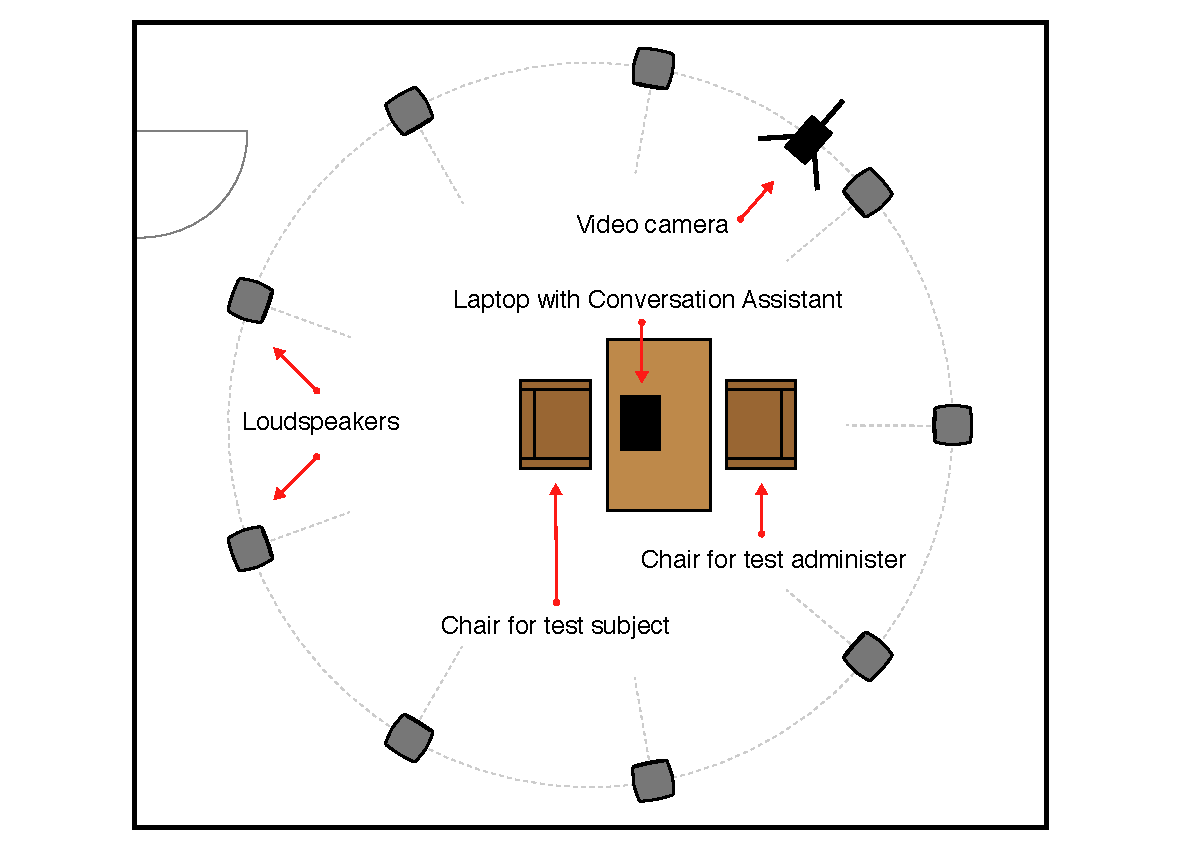
\includegraphics[trim={1.5cm 0cm 1.5cm 0cm}, clip, width=\textwidth]{setup2.pdf}
    \caption{User test setup in the listening room.}
    \label{fig:setup} 
\end{figure}
\begin{figure}[h]
    \centering
    \includegraphics[width=\textwidth]{test2.jpg}
    \caption{A photo of the test environment.}
    \label{fig:photo}
\end{figure}

\subsubsection{Background noise simulation}

In order for the user test situation to better reflect the actual environments and situations where the Conversation Assistant would be typically used, background noise recordings were utilized to simulate a realistic setting. Background noise is one of the critical factors for the whole Conversation Assistant process in two ways: Firstly, noise directly affects how well people can hear and understand speech \cite{pulkki2015communication}, and secondly, noise can drastically affect the accuracy of automatic speech recognition \cite{kallasjoki2016}. Furthermore, the impact of noise on speech intelligibility is generally even more pronounced for hearing impaired persons \cite{healy2016difficulty}, which was also reported by the test participants. \\\\
The uncommonly low background noise level and excellent acoustic properties of the listening room, namely, a short reverberation time of 0,3 seconds, offer a very idealized environment for both listening to speech and automatic recognition of speech. As such, results obtained without the added background noise would apply poorly to real-life usage. During the user tests, background noise recordings proved to be essential for successful testing, as many of the test subjects could hear and understand speech remarkably well with the help of modern hearing aids and cochlear implants, even though they were clinically categorized with severe hearing loss. The background noise level was set to a predefined level at the beginning of each test section, approximately matching the sound pressure level measured at the recording location. The level was adjusted during the test session if needed, in cases where the test participant felt that they could hear too well, meaning that they didn't need to rely on the Conversation Assistant at all in order to follow the conversation. \\\\
The multi-channel audio listening setup installed in the listening room, combined with surround sound recordings in B-format enabled us to accurately and realistically reproduce the surround sound field present at the recording locations. B-format surround recordings are captured using a coincident microphone array, which produces four microphone signals: one omnidirectional ($W$), and three figure-of-eight channels on an orthogonal axis ($X,Y,Z$). These four signals describe the full-sphere sound field at the location of the microphone array, and can be decoded for playback on an arbitrary loudspeaker configuration (though a minimum of four loudspeakers are needed for reproducing the horizontal plane and at least six for full-sphere sound). \cite{furness1990ambisonics, pulkki2015communication} \\\\
The Aalto University Spatial Sound research group provided us with previously made background noise recordings of public places, recorded using a SoundField ST350 portable surround microphone. Each of the two sections of the user test had their own noise environment. The first background is a city street containing mostly traffic noise, recorded near the Havis Amanda statue at the Helsinki Market Square (Kauppatori). The second is a busy cafe located on the Boulevard (Bulevardi) street in Helsinki, containing clamor and noise typical for busy cafes with poor acoustics, as well as some quiet background music. These two environments were selected because they represent locations were conversations often take place, the type of noise is challenging to both humans and automatic speech recognition, and the recordings were consistent in sound and level. \\\\ 
The Directional Audio Coding (DirAC) method developed at the Aalto University Acoustics Lab was used to decode the B-format recordings for the nine-channel symmetrical speaker configuration used \cite{pulkki2015communication, pulkki2006directional}. The DirAC decoder divides the B-format audio file into frequency bands using the Equivalent Rectangular Bandwidth (ERB) psychoacoustic frequency scale. For each frequency band, the B-format audio is then divided into single-channel audio channels for each loudspeaker using virtual cardioid microphones based on the loudspeaker configuration information given to the decoder. Directional and diffuseness analysis is performed for each band and used to adjust the gain and diffusion parameters of each loudspeaker channel within the frequency band. Each loudspeaker signal is then the sum of all the frequency bands for that channel \cite{pulkki2006directional}. \\\\
Using DirAC, the recordings were pre-rendered into nine-channel uncompressed PCM audio files (.wav) for easy playback. Only the horizontal sound plane was used, as it was deemed to be enough for the purposes of the user test. Both audio scenes had multiple recordings of around one minute in length on average, made successively in the same location. For the tests, a constant background noise playing continuously during each test section was needed. Therefore, each pre-rendered nine-channel recording was split into separate mono files for each channel using \href{https://se.mathworks.com/products/matlab.html}{MATLAB}. Then the clips from each channel were edited together to form a longer loop in an audio editing software, and finally combined back to a nine-channel file in MATLAB. The \href{https://cycling74.com/products/max/}{Max/MSP} visual programming language was used to play the resulting nine-channel PCM audio loops. The Max patch consists of a simple GUI for loading the audio file, controlling playback and adjusting the volume, which is presented in figure \ref{fig:max}. \\
\begin{figure}[h]
    \centering
    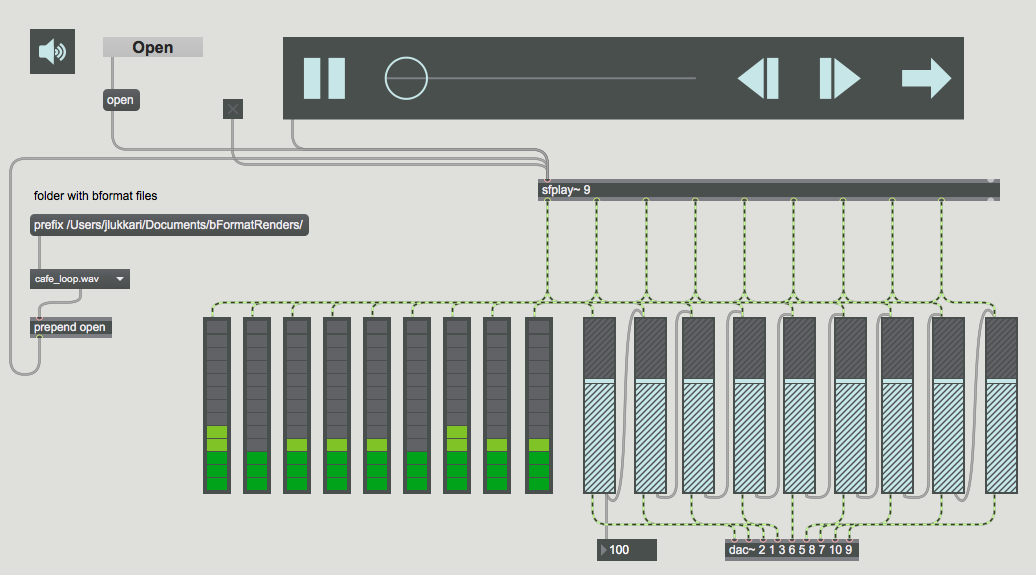
\includegraphics[width=\textwidth]{max.png}
    \caption{Max/MSP patch for playing nine-channel audio files.}
    \label{fig:max} 
\end{figure}

\subsubsection{Test participants}

The plan was for 10-12 test participants. After the preliminary filtering we had ten suitable persons, but ultimately, nine persons were able to participate in the testing. The requirements for the test participants were that they should have some degree of hearing loss, but still be able to communicate using speech. Specifically, a participant could be completely deaf, as long as they were able to answer verbally. The goal was to gather a representative sampling of various levels and types of hearing loss, meaning both deaf and hard of hearing individuals in varying age groups. Potential test participants were contacted through \textit{Kuuloliitto}, a national advocacy group for the deaf and hard of hearing. The test invitation was also shared in various internet forums for the hearing impaired, such as Facebook groups. The relevant background information about the nine test participants is presented in table \ref{table:testsubjects}. There were eight females and one male test subject, ranging from the age of 15 to 74. Two of the test subjects did not report their age, but were estimated to be between 60 and 70 years old. The average age for the seven persons who reported it was 44 years, moving closer to 50 years when including the estimated age for the two others. The test participant group included one student, two retirees, and six employed persons. Two of the participants did not use any major assistive devices (cochlear implant or hearing aid), and were completely deaf. They could however speak and answer questions verbally. Three of the participants had cochlear implants, one in both ears and two in one ear. One of these two used a hearing aid in the other ear in addition to the cochlear implant. Four persons relied on hearing aids, three in one ear and one in both ears. \\
\begin{table}[]
    \renewcommand{\arraystretch}{1.2}  % set row height to 1.2x default
    \setlength{\tabcolsep}{9pt}                % set space between text and cell border
    \centering
    \caption{Test participants.}
    \label{table:testsubjects}
    \begin{tabular}{@{}lcll@{}}
        \toprule
        \textbf{Sex} & \textbf{Age} & \textbf{Status} & \textbf{Assistive devices}                          \\ \midrule
        female       & -            & retired         & hearing aids in both ears                           \\ \midrule
        female       & -            & employed        & none                                                \\ \midrule
        female       & 15           & student         & cochlear implants in both ears, FM system in school \\ \midrule
        female       & 36           & employed        & none                                                \\ \midrule
        female       & 38           & employed        & hearing aid in one ear                              \\ \midrule
        female       & 40           & employed        & cochlear implant, induction loop                    \\ \midrule
        female       & 50           & employed        & hearing aid, induction loop, FM system              \\ \midrule
        female       & 56           & employed        & hearing aid in one ear, FM system                   \\ \midrule
        male         & 74           & retired         & cochlear implant, hearing aid                       \\ \bottomrule
    \end{tabular}
\end{table}

\clearpage

\section{Results} \label{sec:results}

\begin{figure}[b]
    \centering
    \begin{subfigure}[b]{0.45\textwidth}
        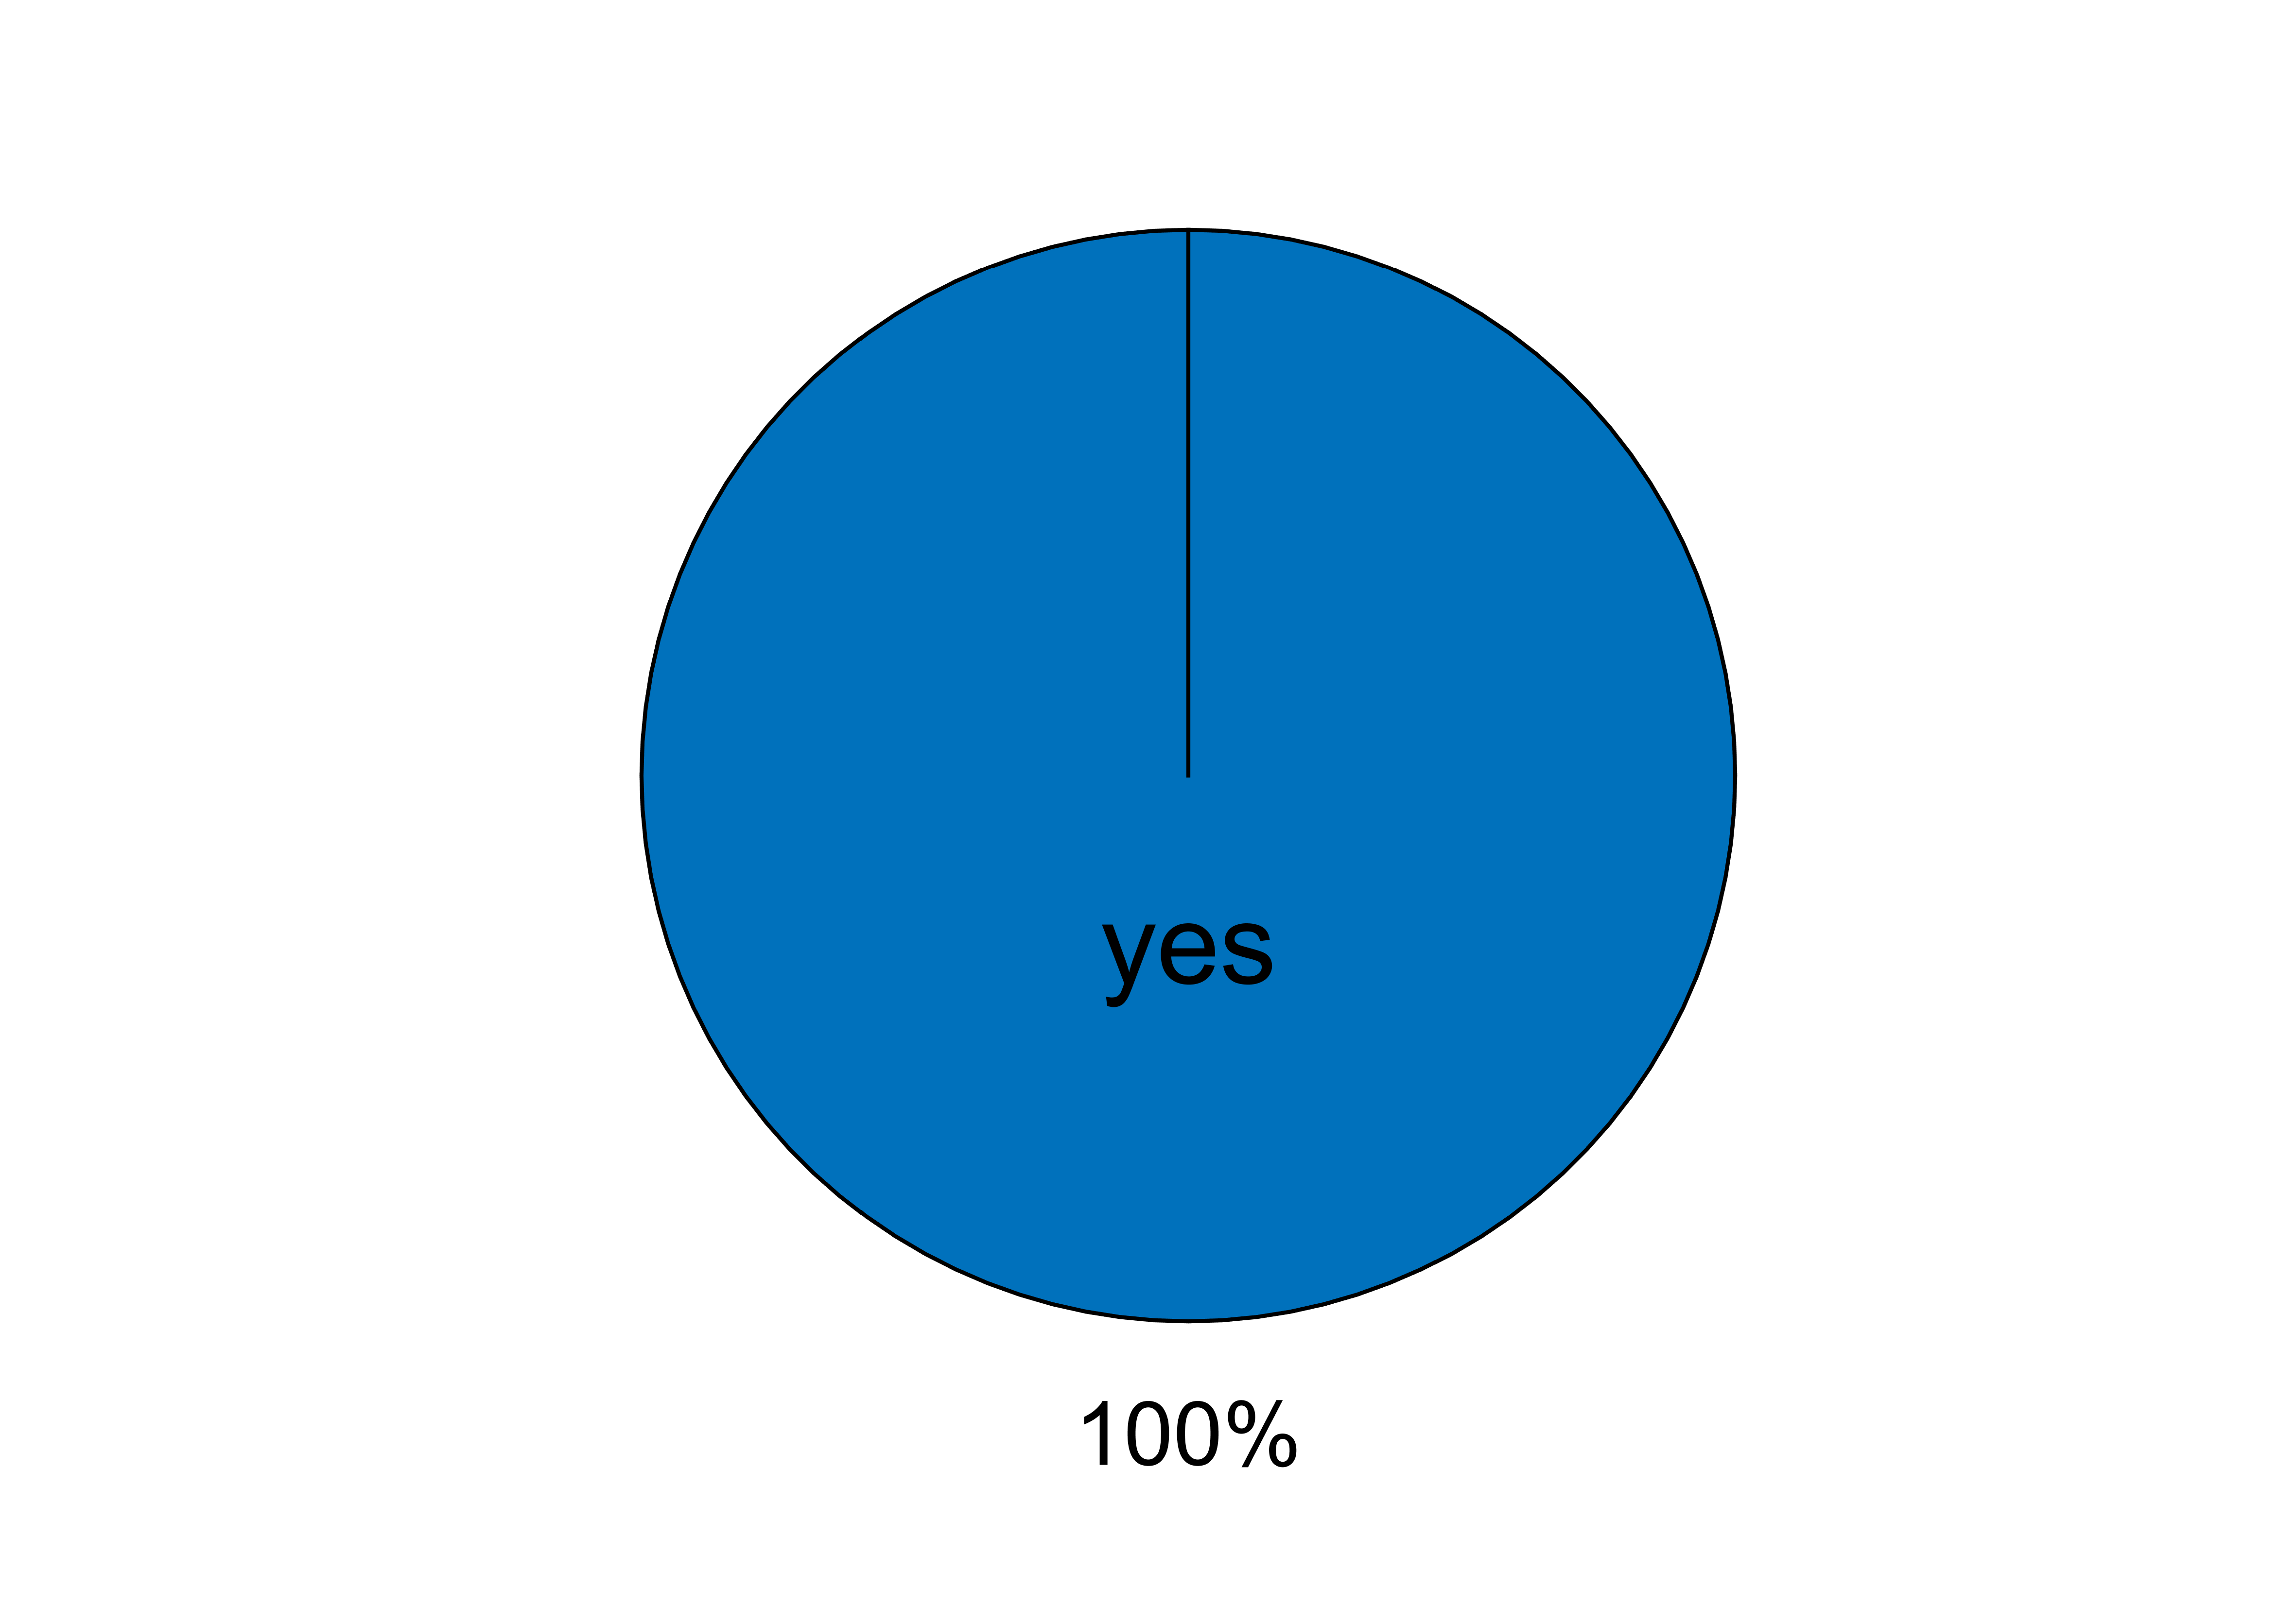
\includegraphics[width=\textwidth, trim={1.5cm 0.6cm 1.5cm 0.2cm}, clip]{T1_1.png}
        \caption*{\textbf{Q5:} "Do you own a smartphone?" \vspace{2mm}}
    \end{subfigure} \hspace{5mm}
    \begin{subfigure}[b]{0.45\textwidth}
        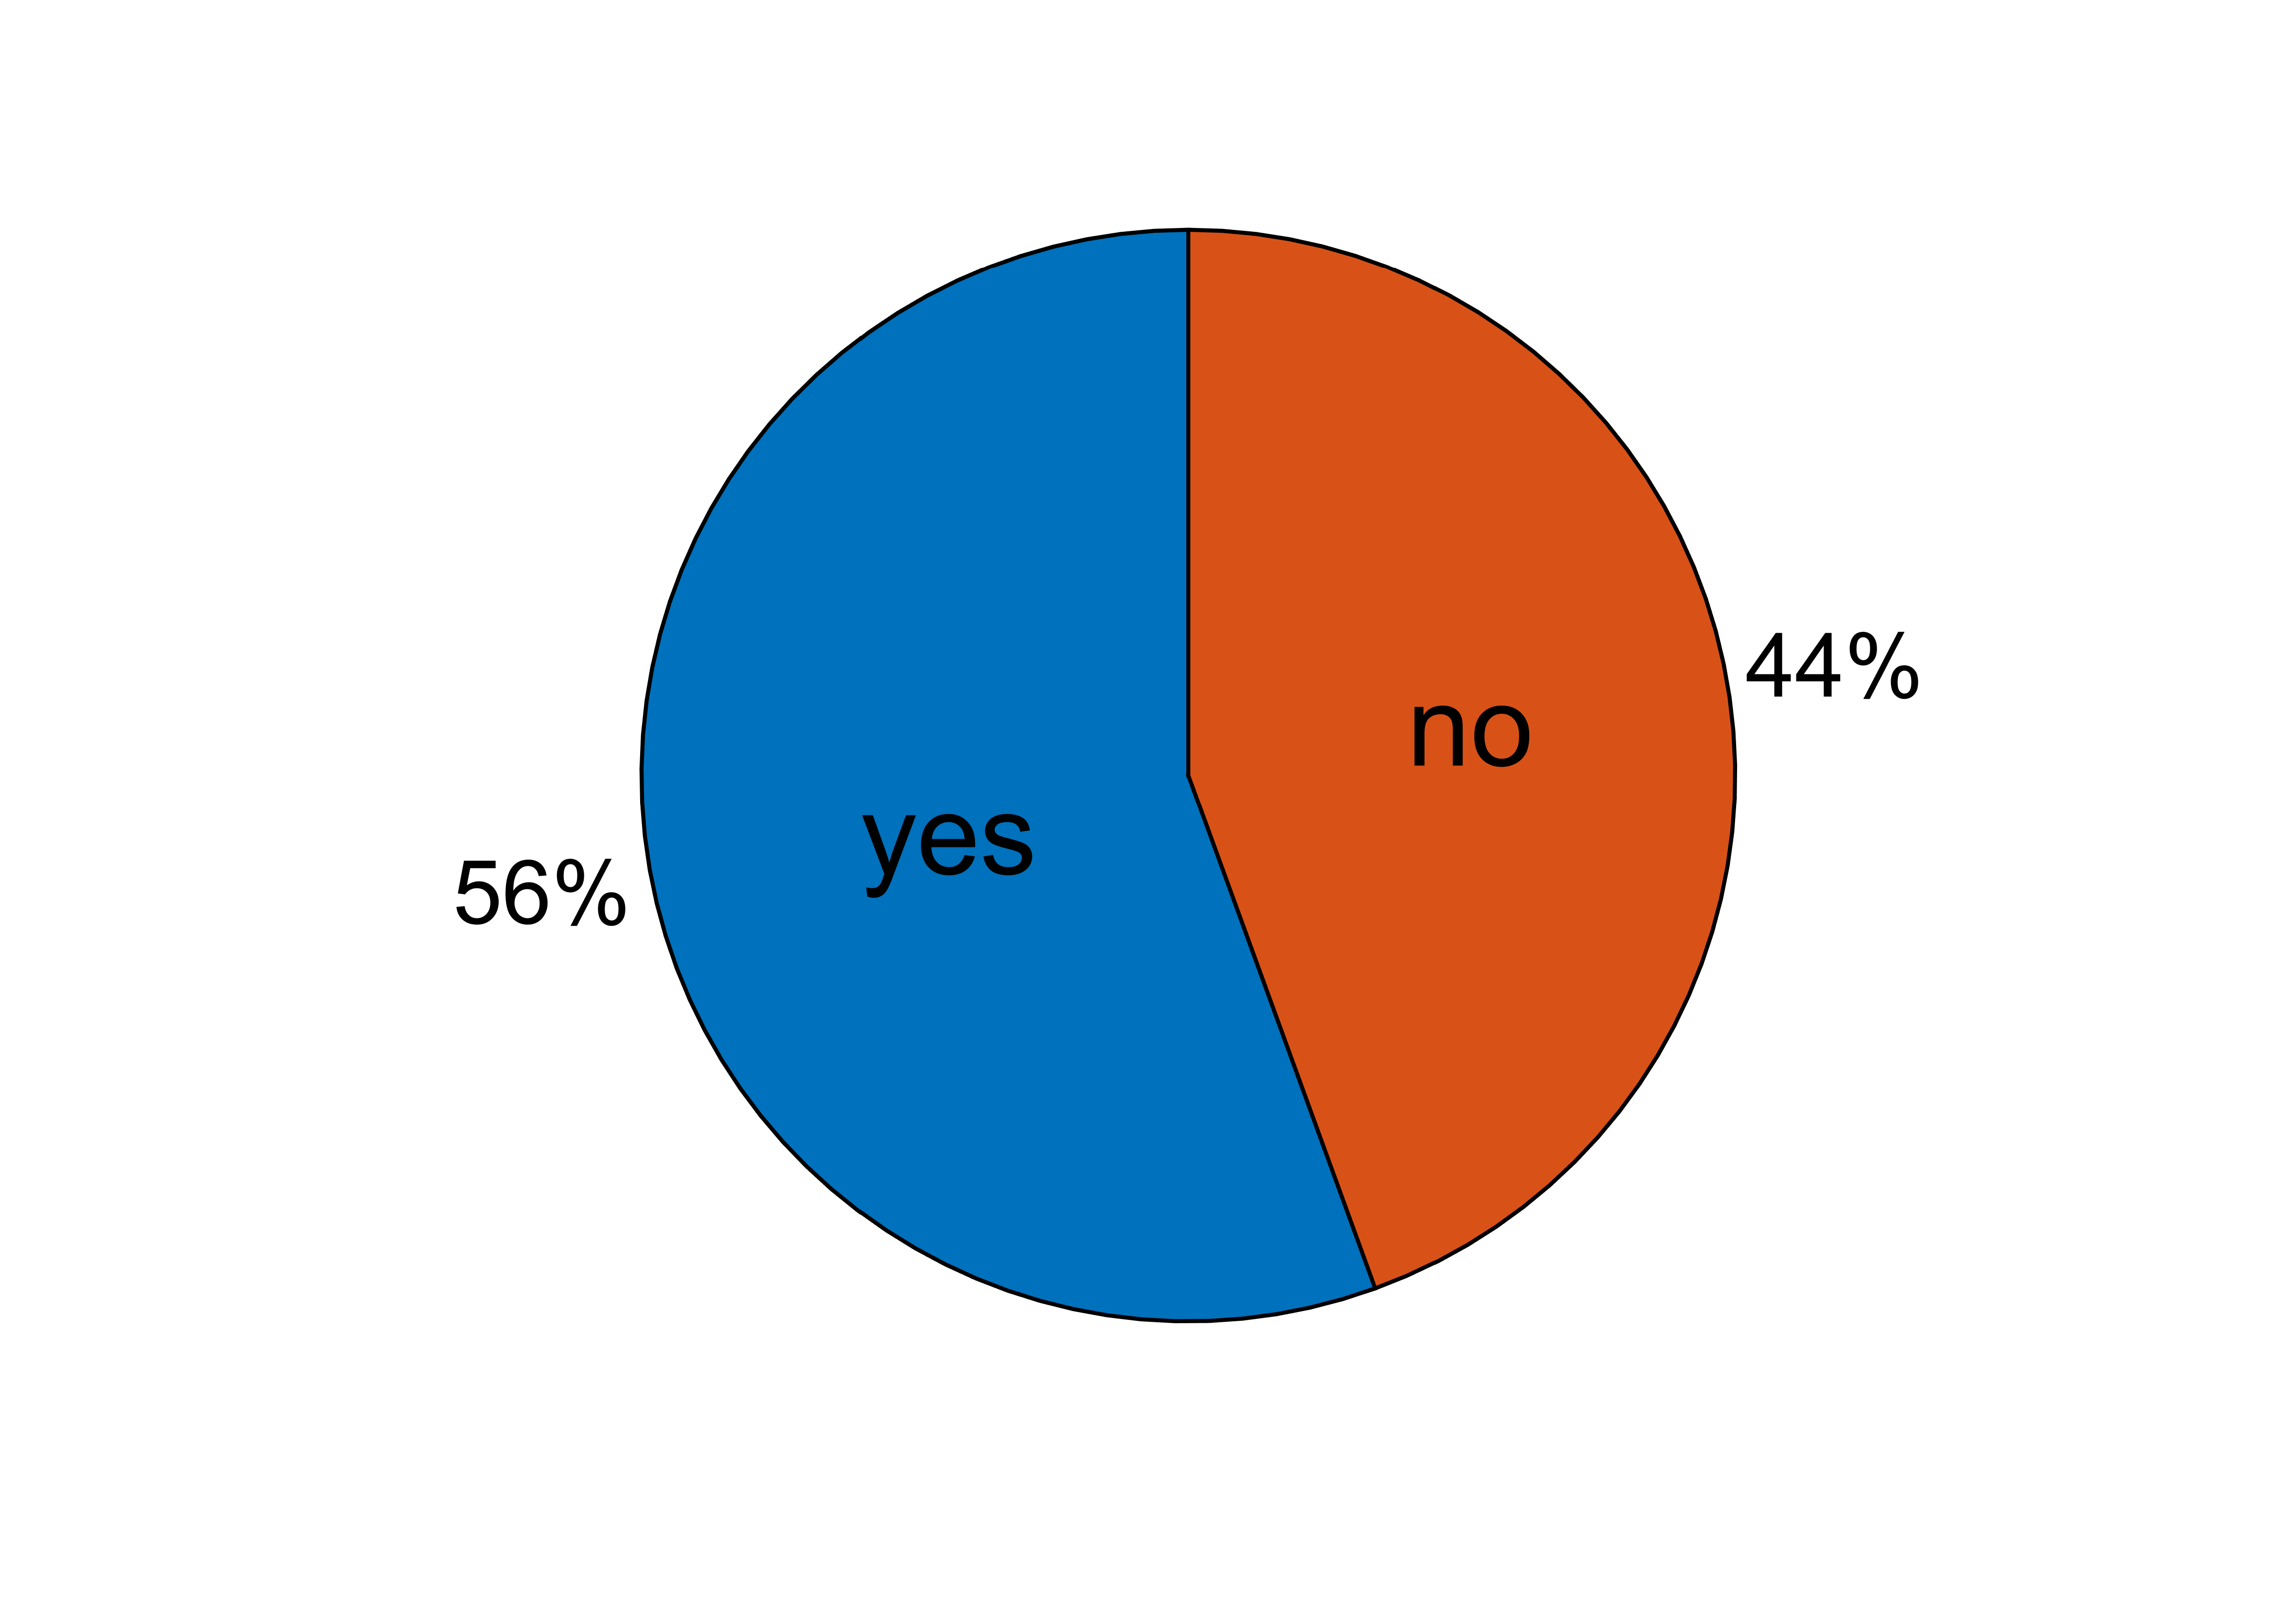
\includegraphics[width=\textwidth, trim={1.5cm 0.6cm 1.5cm 0.2cm}, clip]{T1_2.png}
        \caption*{\textbf{Q6:} "Do you own a tablet?" \vspace{2mm}}
    \end{subfigure}
    \caption{Binary questions Q5 and Q6.}
    \label{fig:results_pie1} 
\end{figure}
In this section, the results obtained from the Conversation Assistant user testing are presented and analyzed. In the user testing, we focused on obtaining a representative opinion of the intended end-users on the overall usefulness of the Conversation Assistant, as well as gathering user feedback on the key areas still in need of improvement. The main objective was to validate the Conversation Assistant approach, or in other words, to answer the question \textit{"is the Conversation Assistant helpful"}. By design, the user test produced qualitative data in the form of subjective opinions and feelings. The MATLAB software environment was used for analyzing the test data, and producing all figures. The reporting of the results begins with the relevant background data gathered. Section \ref{sec:numerical} presents the numerical ratings given by the users, with the data for each of the four test sections presented in its figure. A summary of the written feedback given by the test participants is presented in section \ref{sec:verbal}. In section \ref{sec:analysis}, the results are analyzed and interpreted, and the research questions presented in the beginning are tentatively answered. \\\\
Answers to all binary questions, i.e., questions with a \textit{yes or no} answer, are visualized in figures \ref{fig:results_pie1} and \ref{fig:results_pie2}. The first three of these questions were from the introduction section's background questionnaire (Q5, Q6, Q8), and the fourth from the debriefing section (Q32). All test participants owned a smartphone, and five out of nine owned also a tablet computer. Only 33\% of the test participants reported that they had previously used speech recognition-based applications or services. However, the reliability of this question can be poor since it is not clear if the participants understood what the term means and what services actually use ASR technology. Of the three persons that answered positively, one had used Youtube's automatic captioning, one had used Google Translate's speech-to-text feature, and one had tried speech recognition technology previously in a test session in Aalto University. Eight people corresponded to question 32, with 75\% preferring to pay a one-time payment for this type of application. The reasons given for this preference in the written feedback was quite varying. One person commented that they would not like to pay for it every month in case they end up not using it actively in some months. Another person commented that the monthly payment option could be good if it included all updates and upgrades to the application. The one person who did not answer the question commented that the \textit{Social Insurance Institution of Finland} (Kela) should provide this service for free. One person commented that in general, they would like to first test the application in order to see how well it works before paying for it.
\begin{figure}[t]
    \begin{subfigure}[b]{0.45\textwidth}
        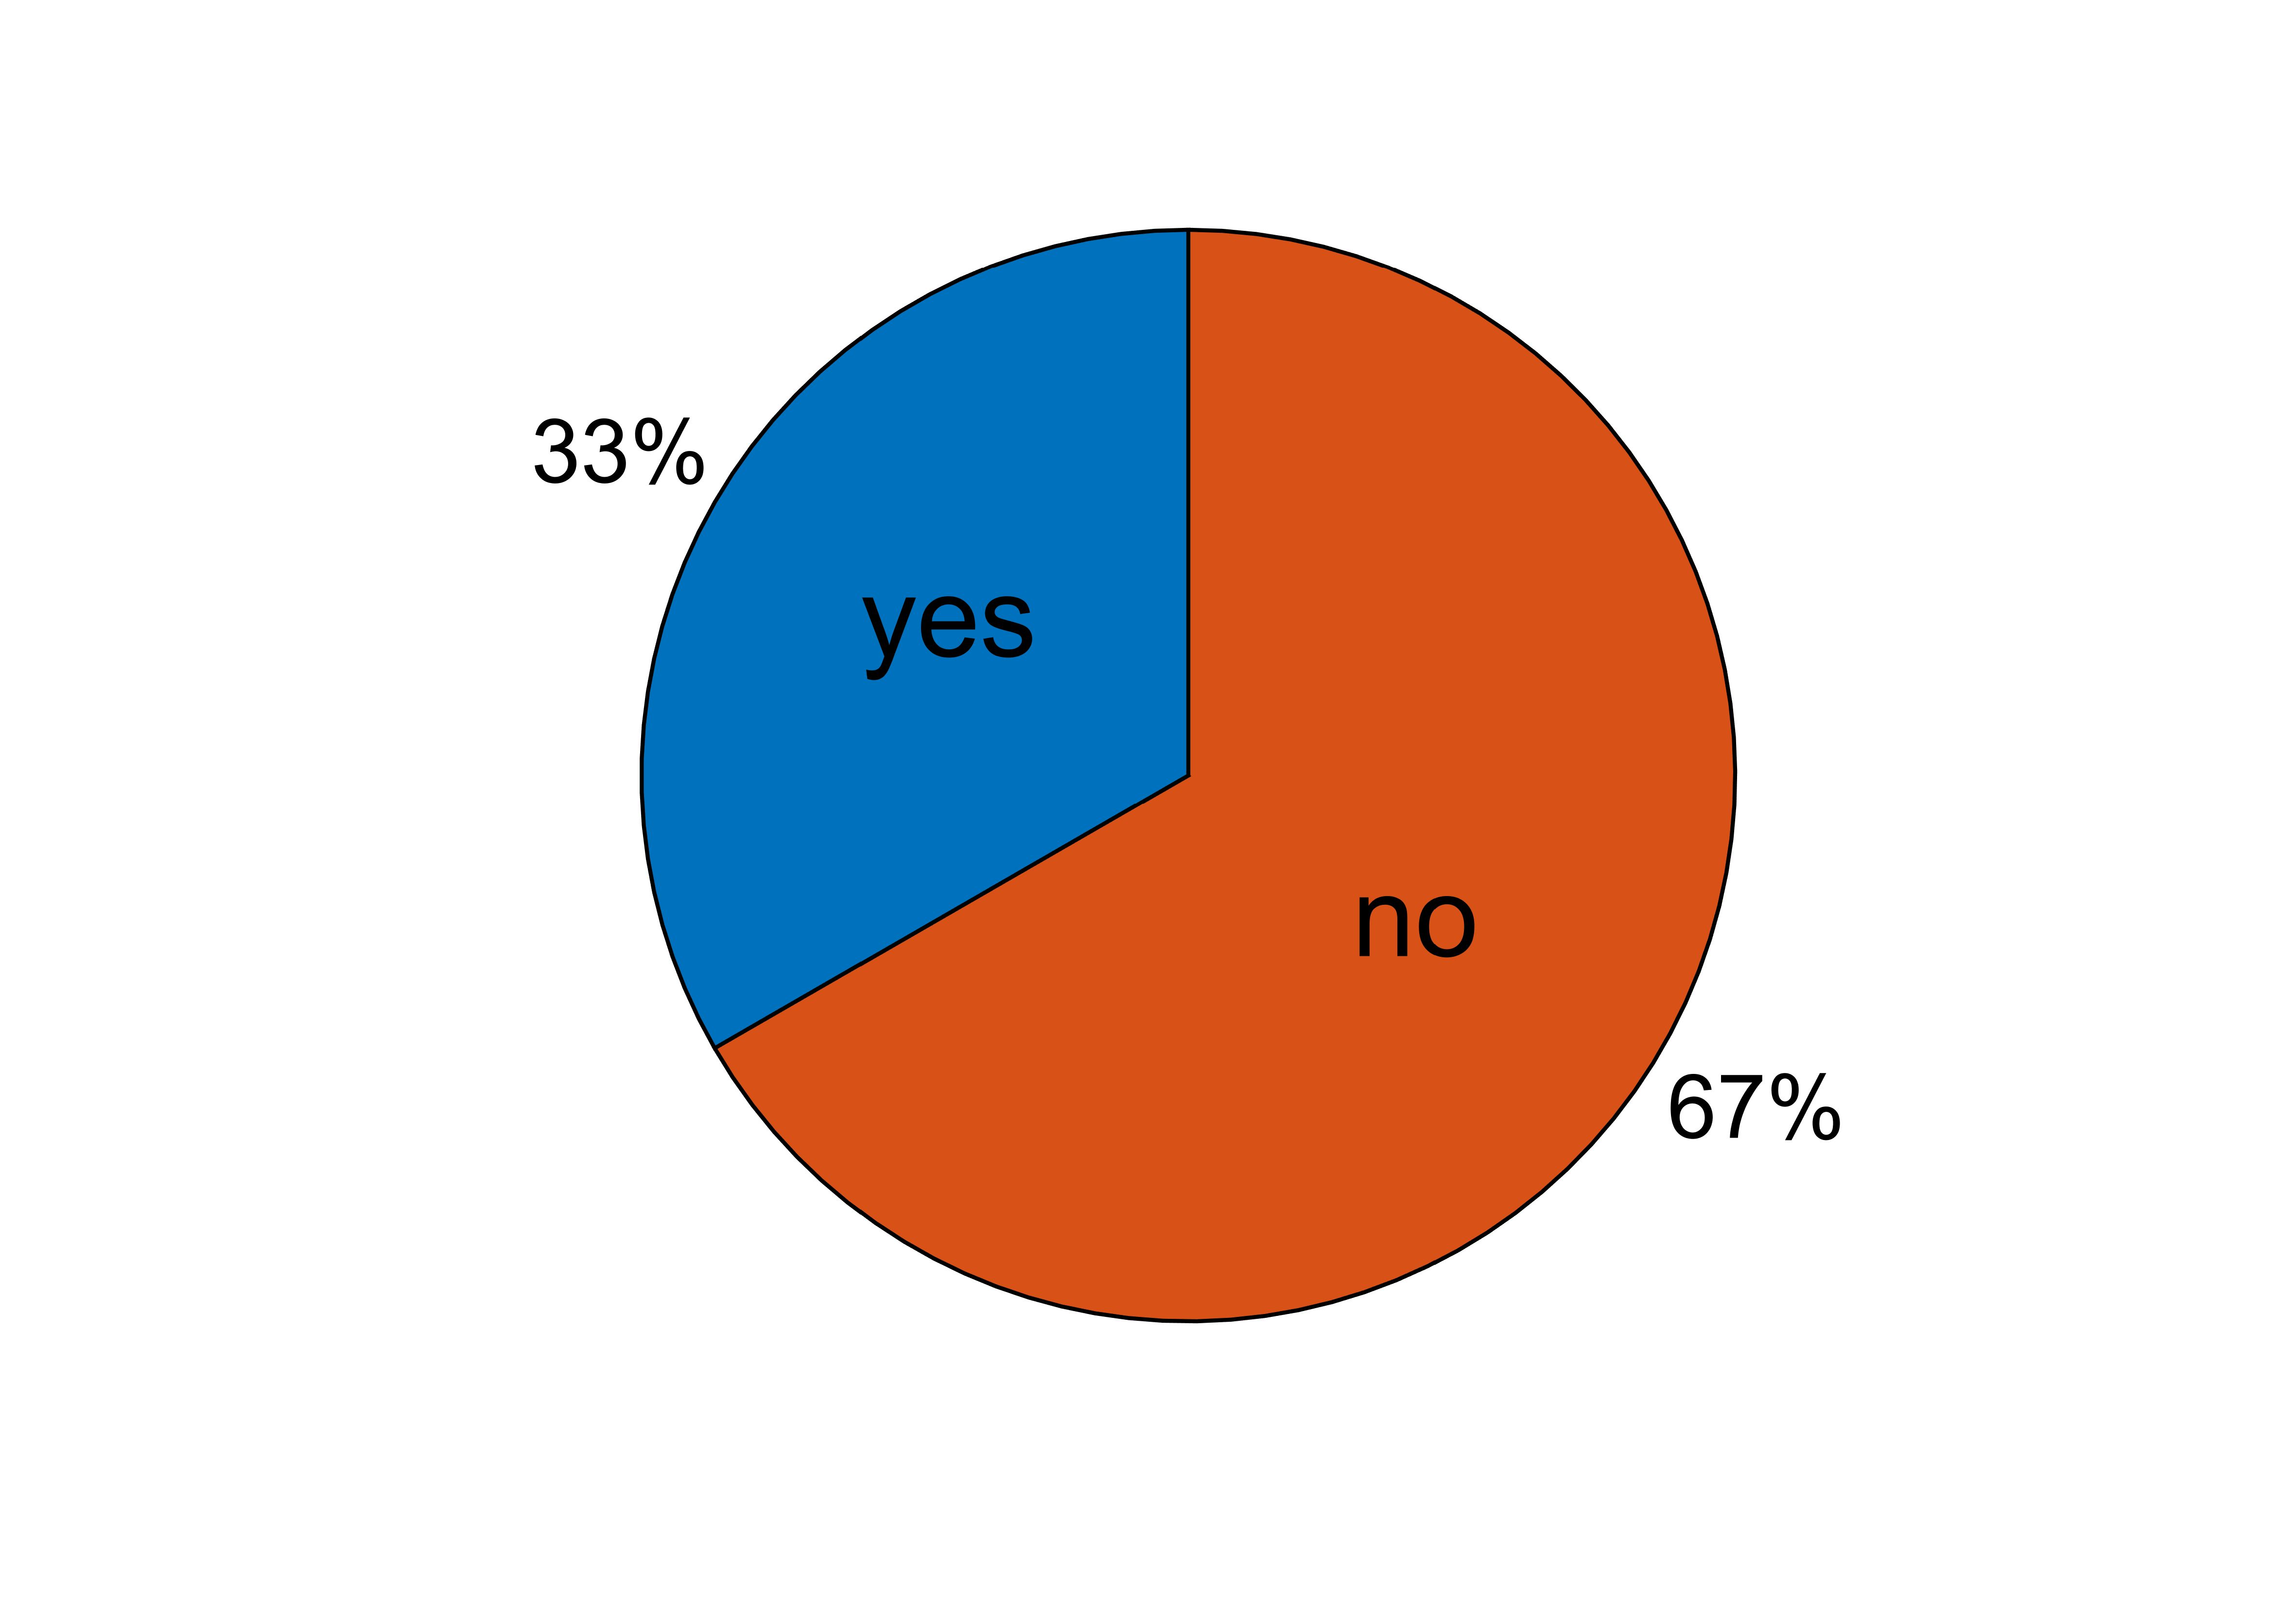
\includegraphics[width=\textwidth, trim={1.5cm 0.6cm 1.5cm 0.2cm}, clip]{T1_3.png}
        \caption*{\textbf{Q8:} "Have you previously used an application or service that uses automatic speech recognition?"} 
    \end{subfigure} \hspace{5mm}
    \begin{subfigure}[b]{0.45\textwidth}
        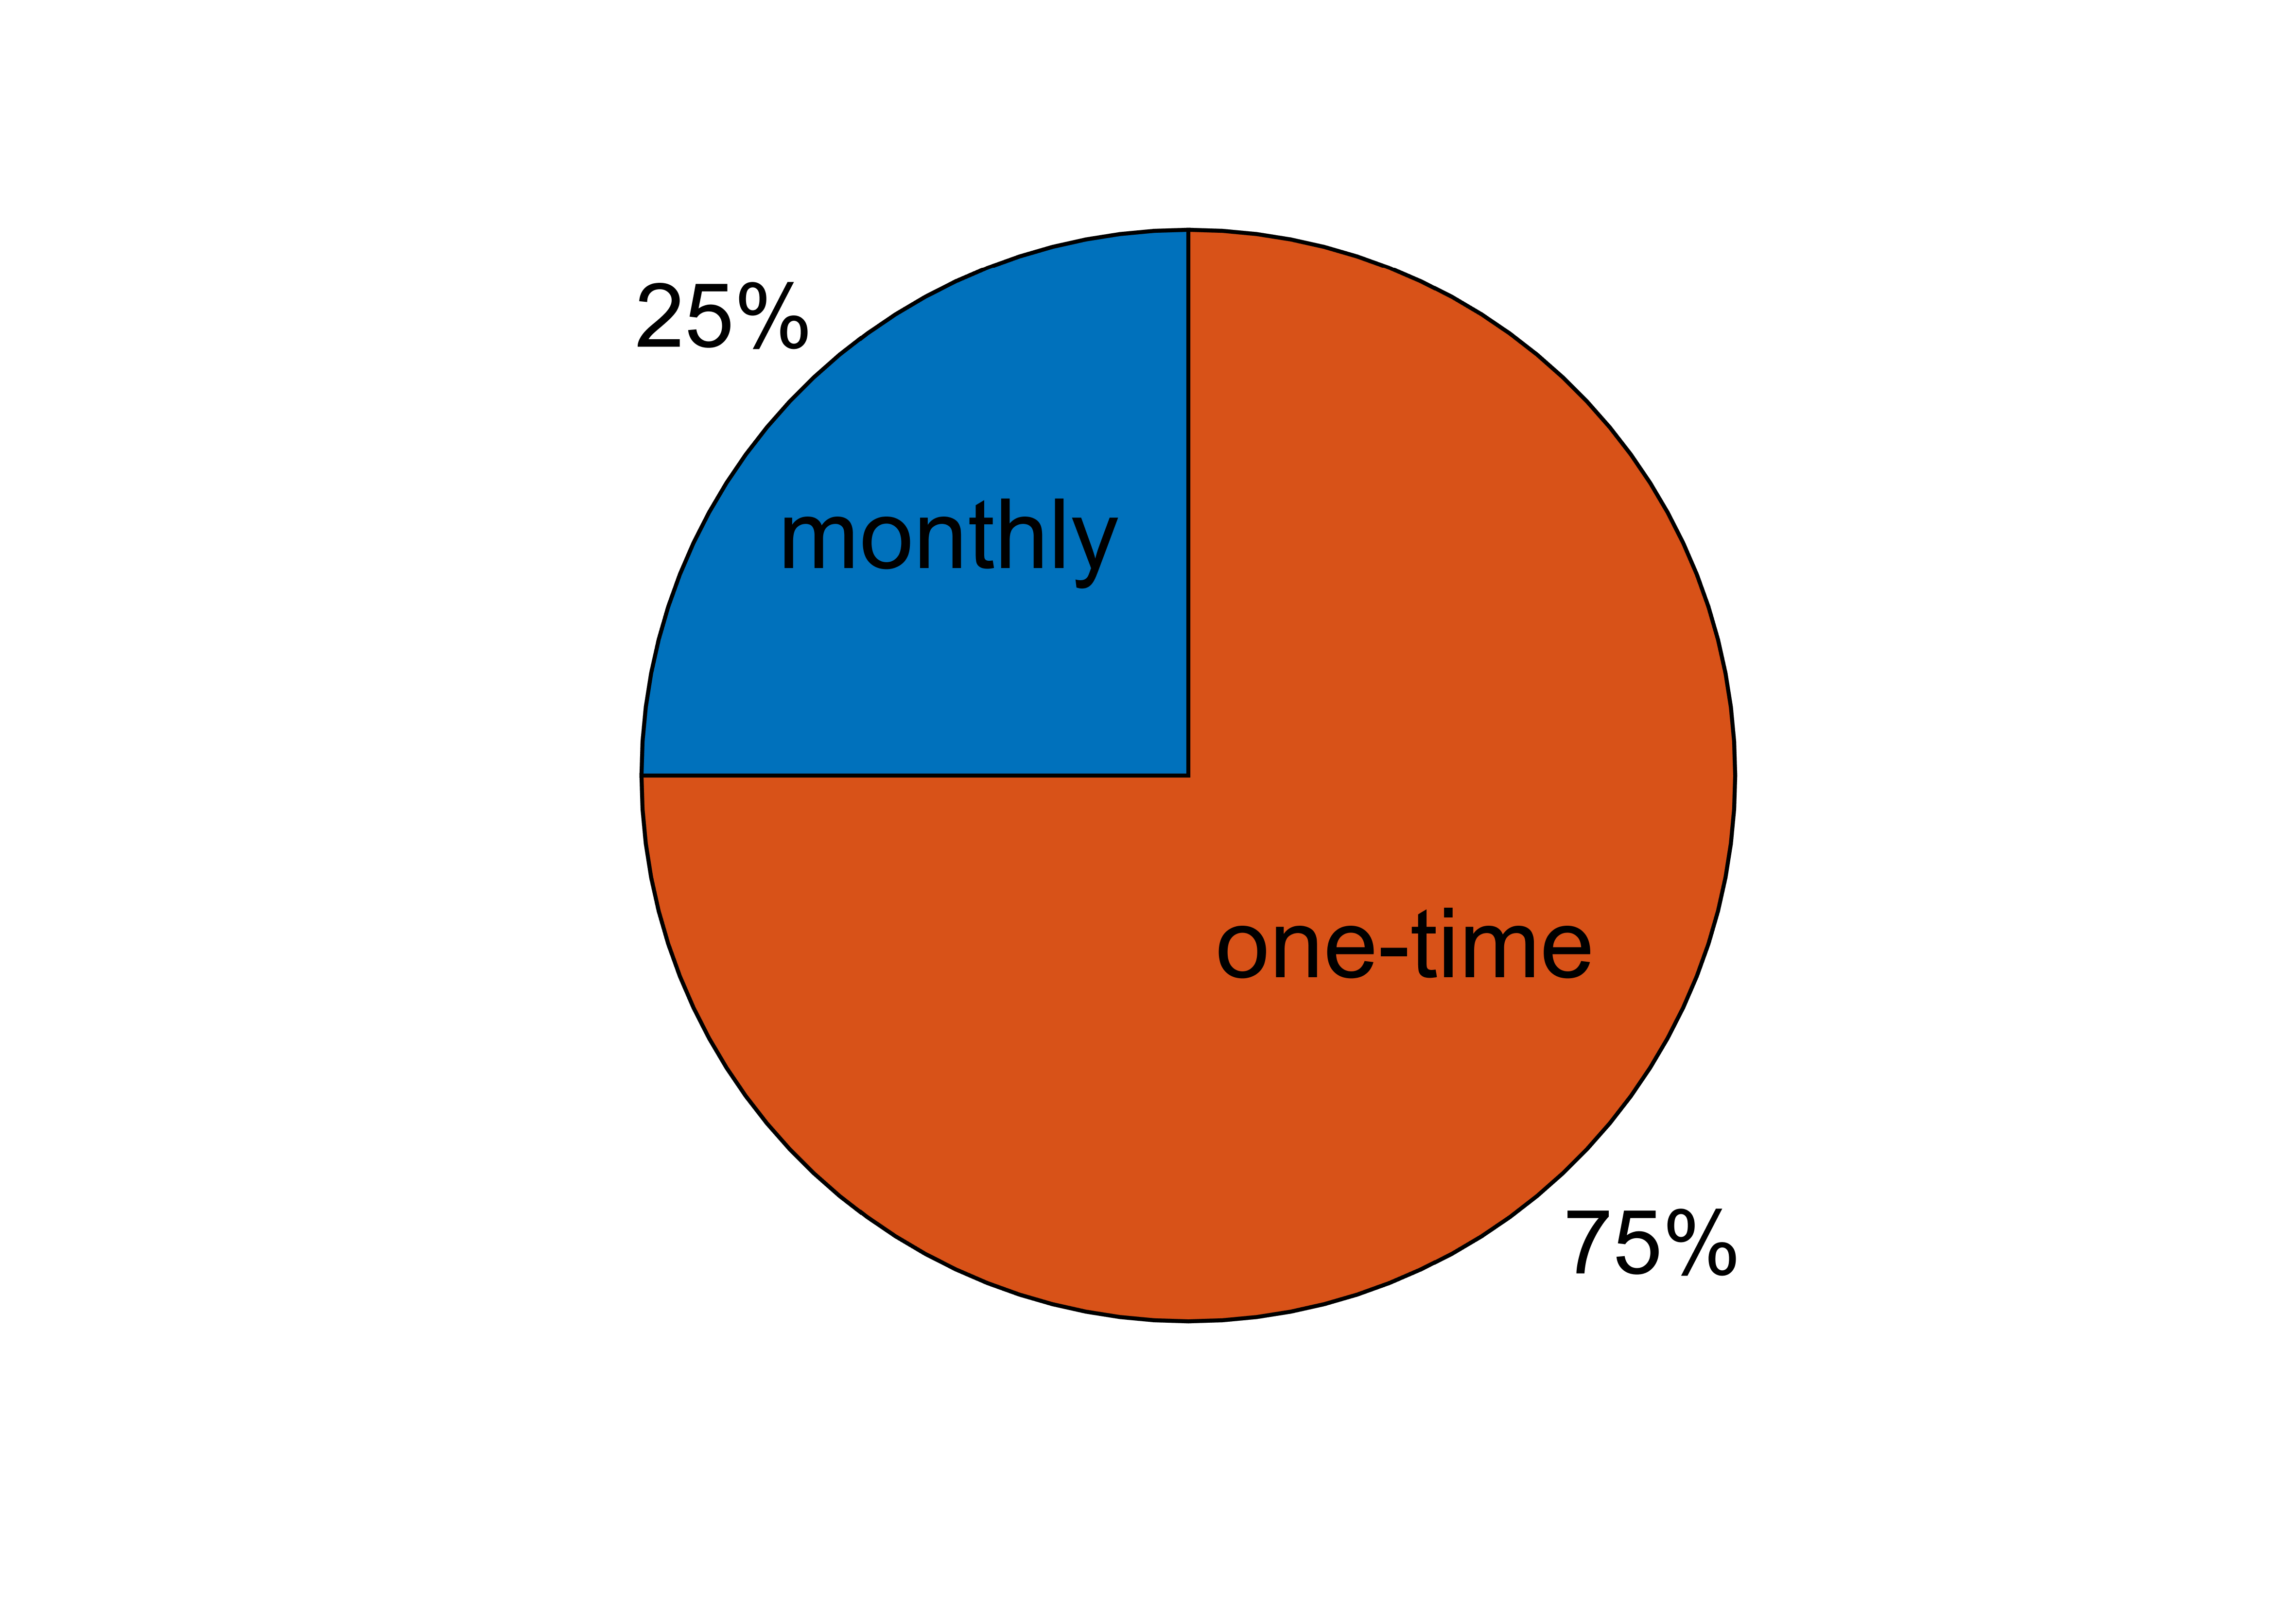
\includegraphics[width=\textwidth, trim={1.5cm 0.6cm 1.5cm 0.2cm}, clip]{T1_4.png}
        \caption*{\textbf{Q32:} "Would you rather pay a monthly fee or a one-time payment for an application like the Conversation Assistant?"} 
    \end{subfigure}
    \vspace{4mm}
    \caption{Binary questions Q8 and Q32.}
    \label{fig:results_pie2} 
\end{figure}

\subsection{Numerical ratings} \label{sec:numerical}

The numerical data obtained, i.e., the numerical ratings given by the test participants, are presented with a box plot for each question, divided by the section. The individual numbers given by the test participants for each question are included in appendix \ref{sec:answers}. In the box plots, the red central mark represents the median value. The bottom of the box (in blue) corresponds to the 25th percentile, and the top of the box to the 75th percentile. It should be noted that when the median is not centered in the box, it shows sample skewness, meaning the values are distributed asymmetrically. The lines in black, extending from the box, display the range of all values that are not considered outliers. A value is judged to be an outlier and marked with a red cross if it is more than 1,5 times the interquartile range (i.e., the size of the box) away from the top or bottom of the box. \cite{boxplot} \\\\
Figure \ref{fig:results1} presents the data from the background questionnaire, which consists only of one question measuring the self-perceived proficiency with computers and mobile devices. 
\begin{figure}[t]
    \centering
    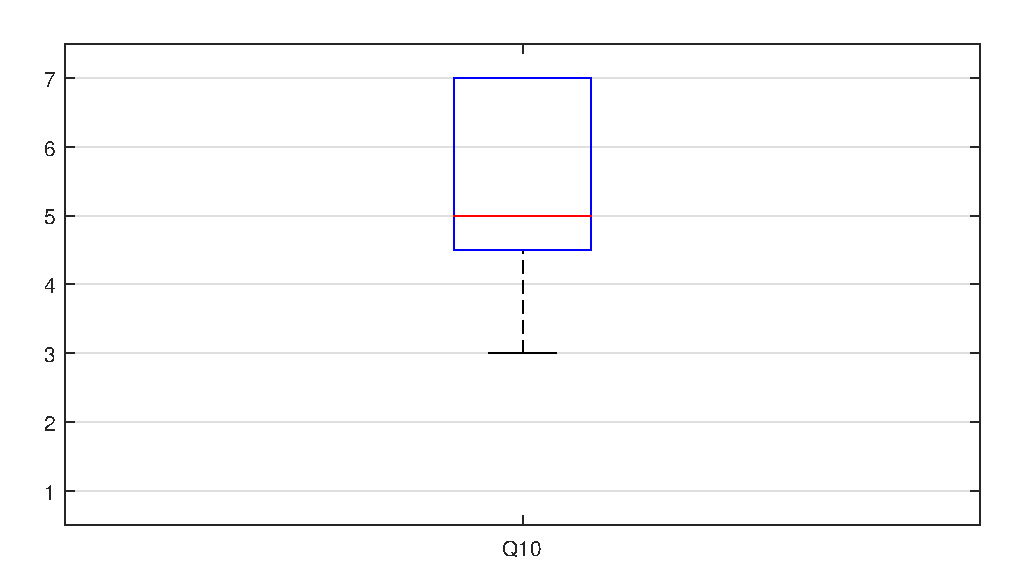
\includegraphics[width=\textwidth]{T2_box1.pdf}
    \caption{Question 10: "In your own opinion, how proficient are you at using computers and mobile devices in everyday life?"}
    \label{fig:results1} 
\end{figure}
The question was included in order to get a rough estimate for how much experience the participant has with these devices and how comfortable they are with technology in general. The subjective wording in the assessment served a purpose as well: Someone who feels that they are good with smart devices likely has a very positive attitude towards technology, regardless of how much knowledge and skill they might actually possess. Conversely, someone who rates their skills very low likely has some aversion and negative expectations towards technology, even if their skills might actually be relatively comparable to someone with a higher rating. Therefore, the answers to this question, together with the other background questions, can be quite useful for better understanding the answers to other questions. \\\\
For example, if an experienced user thinks the application is easy to use, it might not tell that much about its actual ease-of-use, especially from the viewpoint of inexperienced users. If a person with a low reported proficiency thinks it's hard to use, it can be more due to their lack of experience with smart devices together with a somewhat negative attitude, instead of any design flaws in the application itself. With the median value of 5/7, most test participants are arguably familiar with smart devices and relatively comfortable using them. Two of the participants rated themselves at 3/7, while all others rated themselves with a five or higher, with three participants giving themselves the full rating of 7/7. The question also served as a gentle introduction to the questionnaire's format and functioning, preparing and giving the participants some practice with it before moving on to the main questions. \\\\
Figure \ref{fig:results2} presents the ratings from section one of the user test, which was the word explaining task. The questions were the following:
\begin{description}
    \item[Q11] Did the Conversation Assistant help you to understand speech? \\ \textit{(not at all -- very much)}
    \item[Q12] Was using the Conversation Assistant easy? \\ \textit{(not at all -- very easy)}
    \item[Q13] Did using the Conversation Assistant make it harder to follow speech? \\ \textit{(not at all -- very much)}
    \item[Q14] Was the speech recognition fast enough? \\ \textit{(too slow -- fast enough)}
    \item[Q15] Were the speech recognition results accurate enough (speech was recognized correctly)? \\ \textit{(unusable -- good enough)}
\end{description}
\begin{figure}[h!]
    \centering
    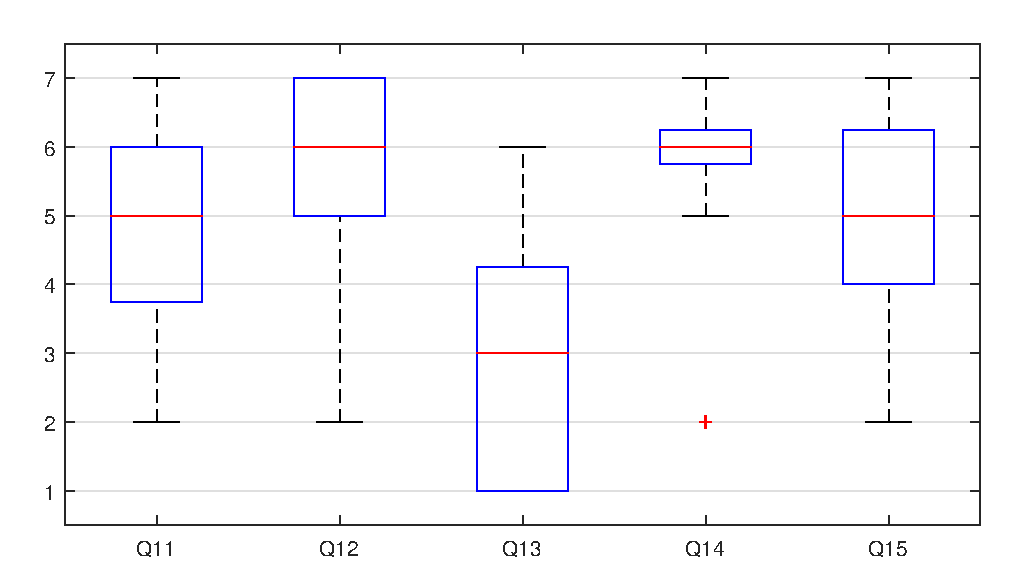
\includegraphics[width=\textwidth]{T2_box2.pdf}
    \caption{Section 1 results.}
    \label{fig:results2} 
\end{figure}
In question 11, the test users seemed to agree that the Conversation Assistant did help them understand speech at least to some extent. A rating of four is the median for values from one to seven, meaning the median of five received can be considered a positive result. Most of the ratings are approximately between four and six, which can be considered a good result. Question 12 indicates that generally the users thought using the Conversation Assistant was easy. Results for question 13 suggests that the Conversation Assistant did make it a little bit harder to follow speech. The range of ratings is quite large, as is the size of the box, meaning the opinions diverged considerably. In question 14, the participants were very unanimous in the opinion that the speech recognizer was fast enough in section one, with one notable exception. Speech recognition accuracy was rated as quite good as well in question 15. \\\\
Figure \ref{fig:results3} presents the data from section two of the user test. The questions were now the following for the free conversation task:
\begin{description}
    \item[Q16] Did the Conversation Assistant help you to understand speech? \\ \textit{(not at all -- very much)}
    \item[Q17] Was using the Conversation Assistant easy? \\ \textit{(not at all -- very easy)}
    \item[Q18] Did using the Conversation Assistant make it harder to follow speech? \\ \textit{(not at all -- very much)}
    \item[Q19] Did using the Conversation Assistant slow down the conversation? \\ \textit{(not at all  -- very much)}
    \item[Q20] Was the speech recognition fast enough? \\ \textit{(too slow -- fast enough)}
    \item[Q21] Were the speech recognition results accurate enough (speech was recognized correctly)? \\ \textit{(unusable -- good enough)}
\end{description}
\begin{figure}[h!]
    \centering
    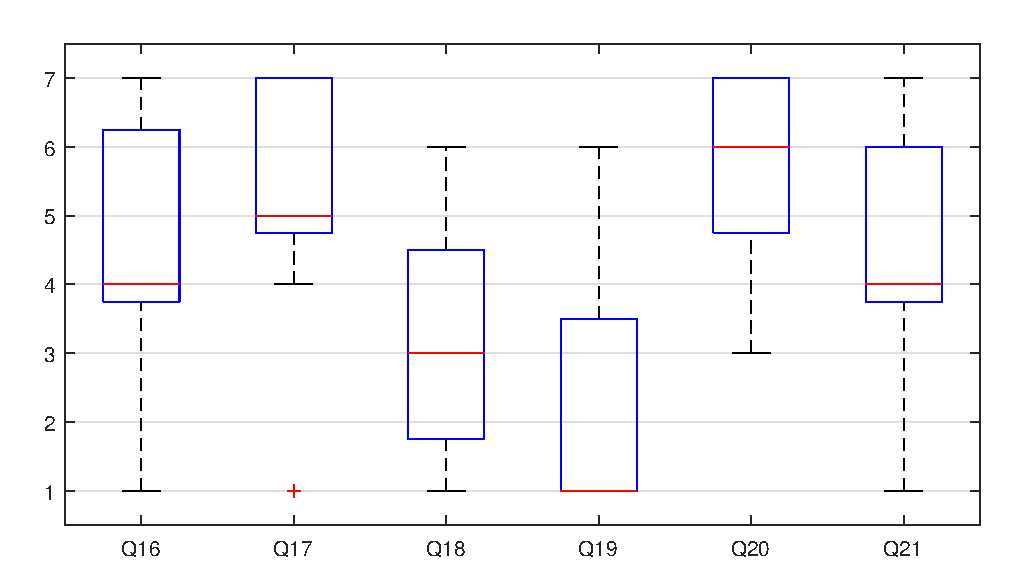
\includegraphics[width=\textwidth]{T2_box3.pdf}
    \caption{Section 2 results.}
    \label{fig:results3} 
\end{figure}
Compared to section one, there was one more question (question 19) relating specifically to conversations. Other questions are the same. In question 16, the Conversation Assistant's helpfulness is rated a little lower on average than in section one, but remains still a positive rating. However, the range of ratings vary all the way from one to seven. Likewise, easiness to use is still rated quite highly in question 17, though there is one disagreeing outlier. Question 18 indicates the Conversation Assistant did make it somewhat harder to follow speech. Question 19 was specific to section two, and asked if the using the Conversation Assistant slowed the conversation. The median is one, meaning the best possible value, indicating that it did not slow the conversation noticeably in the test users' opinion. In one written feedback given to this question, a test participant commented that using it made the conversation faster since it was so easy to follow the speech with the help of the Conversation Assistant. Question 20 asked about the speed of the speech recognition. Again, speed was deemed very good on average with a median of six, and most values within the range from five to seven. Accuracy was rated a little lower this time, but still somewhat positively. In written feedback, the accuracy was also mentioned to be worse than in section one more than once. \\\\
Figure \ref{fig:results4} presents the data from the debriefing. The questions were the following:
\begin{description}
    \item[Q22] Was the Conversation Assistant useful in the test situations? \\ \textit{(not at all -- very much)}
    \item[Q24] In your opinion, is it important that the size and color of the font can be freely adjusted? \\ \textit{(not at all -- very important)}
\end{description}
\begin{figure}[h!]
    \centering
    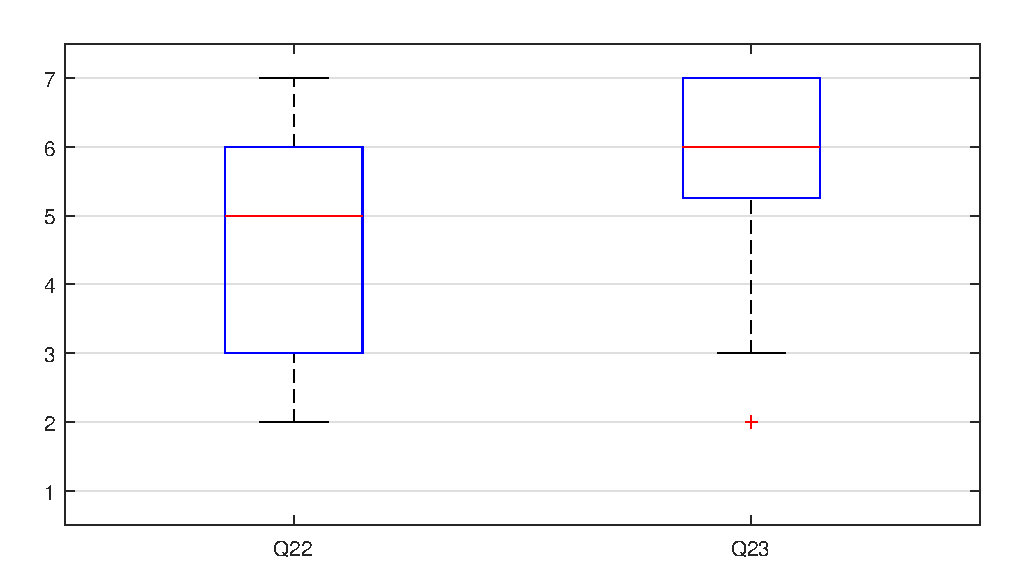
\includegraphics[width=\textwidth]{T2_box4.pdf}
    \caption{Debriefing results.}
    \label{fig:results4} 
\end{figure}
In question 22, the median rating for the overall usefulness of the Conversation Assistant was five, with most values within the range from three to six. A good indicator for a positive result is that no test user gave a rating of one, which corresponded to that it was not at all useful. This can be interpreted to mean that the Conversation Assistant did help all test users at least a little. Also, one test participant gave a rating of seven, indicating that the Conversation Assistant was very helpful for that person. The results are not ideal, but suggests that there is indeed potential in this type of assistive solution. With regards to question 24, most people seemed to think that free adjustment of the font is important, though some commented in the written feedback that while it is good to have as an option, they personally don't feel the need to really change the font size or color that much. Many people commented that for the elderly, who commonly have declined vision as well as hearing loss, or for the visually impaired, changing the font can be very important. \\\\
Figure \ref{fig:results5} presents the results for how much the participants would be ready to pay monthly or as a one-time purchase for an application like the Conversation Assistant.
\begin{figure}[h!]
    \centering
    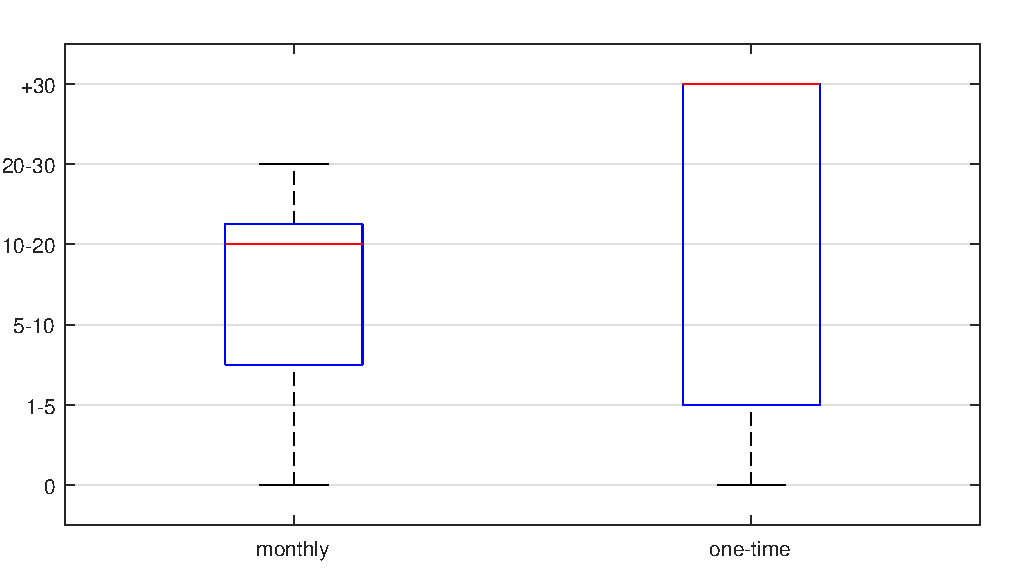
\includegraphics[width=\textwidth]{T2_box5.pdf}
    \caption{"How much would you be ready to pay for an application like the Conversation Assistant?". Price in euros.}
    \label{fig:results5} 
\end{figure}
For the monthly payment type, most people could imagine paying between 10-20€. For the one-time payment option that was much more popular than the monthly option, the answers diverged quite heavily to cover almost all six options. Some would only pay five euros or less, while many would pay more than 30€. In the written feedback, some mentioned that the price they would be willing to pay depends on how well it works. One participant commented that they would pay even several hundred euros if the application is really good. \\\\
Figure \ref{fig:results6} presents a side by side comparison of ratings to the same questions between section one and two. Overall, there does not seem to be major differences between the two sections, with each question getting very similar ratings from both. The ratings for the free conversation appear to be a little worse, with a one rating lower median value in three of the five questions.
\begin{figure}[t]
    \centering
    \includegraphics[width=\textwidth]{comparison.pdf}
    \caption{Comparison of the ratings from section one and two. Ratings for the same question from both sections are grouped together.}
    \label{fig:results6} 
\end{figure}

\subsection{Written feedback} \label{sec:verbal}

Questions 23, and 25 to 29 were written-answer questions. A summary of the answers for each question is provided here. Likewise, the optional written comments given to the numerical rating questions are summarized. In question 23, the participants were asked to explain their overall rating for the usefulness of the Conversation Assistant. Among the comments were the following:
\begin{quote}
    \centering
    \renewcommand{\baselinestretch}{1.4}
    \textit{
    "It created a safety net", \\
    "Obviously it was useful when one can't hear", \\
    "I could hear most speech so I did not need it very much", \\
    "It was very useful because of the background noise", \\
    "Too many errors in the text, can't rely on it to give correct information", \\
    "I'm used to lip reading, so using the Conversation \\ Assistant would require some getting used to".}
\end{quote}
\vspace{1mm}
Question 25 asked what was good in the prototype. The comments included:
\begin{quote}
    \centering
    \renewcommand{\baselinestretch}{1.4}
    \textit{
        "I could keep up with speech", \\
        "Clear to use. Would not attract attention if used for example in meetings", \\
        "It typically captured the key words from the speech", \\
        "At least it tried to keep up with speech all the time", \\
        "Even if it got only a few words from the speech, \\ \vspace{-2.5mm} it did help to confirm that I had heard at least something correctly", \\
        "Good that works in Finnish. Enables following speech \\ \vspace{-2.5mm} in situations where I can't see the speaker", \\
        "It supported my hearing well, I could look away and \\ still keep up with speech from the history".}
\end{quote}
\vspace{1mm}
In question 26, the participants were asked what should be improved in the prototype, to which the answers given included:
\begin{quote}
    \centering
    \renewcommand{\baselinestretch}{1.4}
    \textit{
        "Less errors", \\
        "The text could be bigger", \\
        "Extra words could be removed", \\
        "Still quite a lot of errors", \\
        "Some sentences were wrong", \\
        "Speech recognition should be improved a lot" \\
        "The text was too fast at times, could be a little slower. \\ Somethings were missing at times".}
\end{quote}
\vspace{1mm}
Question 27 asked what features the participants would like to have in an application like the Conversation Assistant, to which the comments included:
\begin{quote}
    \centering
    \renewcommand{\baselinestretch}{1.4}
    \textit{
        "That it would be always available and usable in a mobile phone", \\
        "Separate colors for different speakers", \\
        "Store the conversation history", \\
        "Available as a mobile application", \\
        "Speed and vocabulary could be better", \\
        "Could be used for internet videos and Skype meetings", \\
        \vspace{2mm}
        "Would be available to both phones and computers".}
\end{quote}
\vspace{1mm}
In question 28, the participants were asked if they would like to use this type of application, or if they already used one. The comments included the following:
\begin{quote}
    \centering
    \renewcommand{\baselinestretch}{1.4}
    \textit{
        "I would definitely use", \\
        "I would use at work. I have wanted to use one, \\ \vspace{-2.5mm} but have not been able to find a suitable application", \\
        \vspace{2mm}
        "I would even buy a half-finished version, \\ if there only was one available in Finnish".}
\end{quote}
Overall, four people directly indicated that they would like to use this type of application, were there one available. Some people did not answer the question of would they use, only answering that they had not used one before. This question could have been better implemented as two separate question to get an answer from everyone to would they want to use it. Finally, question 29 asked that in what situations would you use it, to which the answers included:
\begin{quote}
    \centering
    \renewcommand{\baselinestretch}{1.4}
    \textit{
        "In many situations. Generally when communicating with others", \\
        "With my family and friends. At the workplace", \\
        "At the workplace in Skype meetings, and when watching \\ \vspace{-2.5mm} the TV when it does not have captions", \\
        "I would keep it running at work just in case. In  \\ \vspace{-2.5mm} situations with many people, like restaurants. In a car", \\
        "For example in noisy places", \\
        "In normal conversations with friends and family", \\
        \vspace{2mm}
        "In meetings and school lectures".} \\
\end{quote}
Based on these comments, the Conversation Assistant seemed to be useful for most participants. Availability as a mobile application was a common desire. People liked the transcription history view. The optional written feedback to the numerical rating questions also included some valuable comments. One person mentioned that the user interface layout could be flipped upside-down to make it easier to follow both the speaker and the screen simultaneously. One person commented that they tended to first listen to the speaker in full, and only then look at the screen.

\subsection{Analysis} \label{sec:analysis}

Overall, the results of the user testing can be considered positive. Even though the number of participants was relatively low, the ratings and feedback given seem to clearly validate the Conversation Assistant approach as helpful for the hearing impaired. Based on the written feedback, the level of usefulness provided by the simple prototype was already sufficient for many people to express desire towards using it in practice in their own everyday life. The speech recognition accuracy was generally considered to be the limiting factor for usefulness in an otherwise well-functioning application. Therefore, speech recognition accuracy should be primarily improved for increased utility. Good ratings for the easiness to use indicate that the simple user interface design style and basic layout of the elements was suitable. The Conversation Assistant seems to make speech a little bit harder to follow on average, but this was to be expected. Having to divide attention between the speaker and the screen has previously been shown to be distracting in \cite{kushalnagar2015tracked}. The rating for the distraction could be more meaningfully understood when compared to the same rating for a human translator. The conclusion is that ideally, the application's text display style and position should be designed in a way that would limit the visual dispersion between the speaker and the screen. For quantifying visual dispersion, Kushalnagar et al. suggested using eye-tracking to measure how much the user has to move their eyes between the two visual sources. \\\\ 
Some people commented that due to the simplicity of the conversational situation, they did not need the Conversation Assistant as much as they possibly would in other situations. Some of the test participants also reported that they could hear pretty well in spite of the background noise. Some were accustomed to using lip-reading, which they could rely on instead of having to watch the Conversation Assistant, and glancing at the Conversation Assistant distracted from lip-reading. One major observation is that the speed of the speech recognition was clearly deemed to be fast enough. Speech recognition accuracy got a relatively good rating as well in both sections, though many mentioned in the written feedback that there were a lot of transcription errors especially in the conversation task. A sufficient recognition speed rating means that all future effort can be put towards improving the accuracy of the ASR system, instead of having to try to also optimize for the recognition speed at the same time. One occurrence worth mentioning is that one of the two completely deaf test participants was able to correctly answer all word descriptions in the word explaining task, which many of the much better hearing test participants could not do. This observation gives more supports for the usefulness of the Conversation Assistant, as a deaf person was able to correctly understand descriptions for words only by reading them from the Conversation Assistant's display. Of course, mental acuity does likely affect the results to some degree, and even though the words were the same for everyone, the descriptions varied slightly from person to person. \\\\
There are some potential error sources and human biases that have likely somewhat affected the results. One factor to keep in mind when analyzing the results is that the people who participated in the testing showed enough interest towards the Conversation Assistant to take part in the testing in the first place, meaning the test participants have to be viewed as inherently positively biased towards the Conversation Assistant in some small degree. It seems probable that someone with no interest towards this type of assistive application would most probably not participate in testing it either. As mentioned, section one and two used different background noise recordings, which might have also affected the results slightly. For the pricing questions, the answer price ranges were mistakenly written with inclusive ranges between different options, instead of exclusive ranges, meaning the different options were not completely unambiguous. For example, if a test user wanted to answer \textit{"ten euros"}, there was two possible categories to choose from, which both included this price. It is possible that this could have skewed the pricing results a bit into either direction. The test situation used corresponded to one particular type of use scenario, meaning the results obtained may not fully apply to different settings. More testing in different situations, such as in group conversations or lectures  is needed for comprehensive validation. 

\section{Conclusions} \label{sec:loppu}

In this work, a conversational assistance application was investigated as a solution to the spoken communication challenges hearing impaired individuals have. In the investigated method, deaf and hard of hearing people are supported in conversational situations by providing real-time speech-to-text transcriptions. A prototype application was implemented for testing the validity and usefulness of the proposed method with current speech recognition technology. A user test was designed and executed for obtaining results to these questions. The user test situation simulated a typical conversation between two persons, but one of the persons had the Conversation Assistant prototype for support, in addition to the possible hearing augmentation devices they normally have. Background noise recordings were used to match a realistic acoustic use environment. Realistic background noise was important, since the speech perception ability of an individual with hearing loss typically decreases noticeably in noisy and reverberant acoustic environments. The results indicate that the Conversation Assistant can help hearing impaired people to understand and participate in conversations. Based on the results and feedback obtained, the usefulness of the Conversation Assistant seems to depend in large part on the quality and accuracy of the speech recognition results. \\\\
This first round of user testing also ended up being the only one. At the beginning of the project, two or more rounds of testing were originally envisioned. However, after the first round of testing, more iterations of the same test setup were deemed redundant without significant changes to the Conversation Assistant, which in turn was not possible within the scope of this thesis. Expanding the test setting from a one-on-one conversation to a group conversation situation would have been the ideal next step. Many test participants reported that one-on-one conversations can be relatively easy to follow, when they can see the other person well. This in turn led many of the test subjects to speculate that the Conversation Assistant would be much more useful in group conversations and in situations where the speaker is farther away, or lip-reading is otherwise not possible. Examples given of the latter situations included lectures and video-conferencing meetings. \\\\
During the user testing, one of the test participants brought a written language interpreter, as the person was complete deaf. This offered a good opportunity to informally compare the Conversation Assistant side by side with a human, professional speech to text transcriber. The translator had a laptop computer that was placed next to the Conversation Assistant laptop on the table in front of the test user. The translator had a wireless keyboard that she used to write text to the screen, and the end result was effectively and visually very similar to the Conversation Assistant. During the introduction phase and between the test sections, both laptops were simultaneously displaying transcriptions, the other produced by our ASR system, and the other by the human translator. Of course, the human translator paused during the actual testing. Based on this brief empirical observation, the Conversation Assistant seemed to be noticeable faster than a human translator, but accuracy was still relatively far off from a human translator for conversational speech. However, it was interesting to note that the human translation results were far from perfect as well, containing surprisingly many errors in the spelling. The most probable explanation seems that accurate translation has to be sacrificed for speed. All things considered, the Conversation Assistant didn't appear to be too far off from the performance level of a professional human translator. One area, where human translators are by far superior is that they can easily add relevant information to the translation, such as who is speaking (to whom), describing the mood or tone of voice, and also translate other sounds in addition to speech. While a human translator still seemed to be better overall in speech-to-text translation for the hearing impaired, it takes many years of training and practice for a human translator to achieve these results. Also, one person cannot be in many places at the same time, and requires monetary compensation, meaning only a limited amount of people can benefit from those translation services. On the contrary, once ASR models are trained, they can be copied infinitely and used everywhere with practically no additional costs. This way, utilizing ASR can enable the current best achieved level of automatic speech recognition for all very cheaply. \\\\
Potential objective measurements considered for the user test included eye-tracking, which could have been used to accurately determine the percentage of time the users spend watching the Conversation Assistant screen instead of the person speaking. Eye-tracking could also be used to assess how people tend to use the Conversation Assistant: Do they look back-and-forth quickly between the speaker and the screen, or do they first try to listen a full sentence watching the speaker, and only after that check the screen for help. The User Interfaces research group at Aalto has experience in eye-tracking measurements, and could have provided the necessary equipment if desired. While this information would be interesting from a HCI point-of-view, and have some implications for the UI design and recognition result displaying, it did not answer significantly to the primary and secondary objectives set out for the tests at this stage. It is also possible to obtain a decent approximation for this data by analysing the video recordings made of the test session, which can also show were the test subject was looking at on any given moment during the test. To avoid manually gathering this data from the video, computer vision methods for eye-tracking could be used to get quite accurate results automatically. For example, Krafka et al. used deep convolutional neural networks for successfully tracking eye movement on mobile device cameras \cite{krafka2016eye}. However, this was left for future work due to time constraints. \\\\
Ultimately, it is the subjective experience of the end users that matters when evaluating the usefulness of the Conversation Assistant. Typical objective measurements for ASR performance, like the word error rate may not be the most relevant: A better word error rate does not automatically mean that the quality of the recognition result is also better in terms of understanding the contents \cite{wang2003word}. Also, the end-goal of the Conversation Assistant is not to have perfect transcriptions of speech, but to support and supplement the user's hearing in real-time conversational situations. If the user can understand everything spoken to them with the help of the system, even though the text is full of errors, then it is succeeding in its intended purpose regardless of the speech recognition accuracy. Consequently, in real-time situations the type of errors is generally much more important than simply the overall percentage, when it comes to understandability and helpfulness \cite{wang2003word}. This observation feels inherently logical for conversations: It is easy to imagine that a few extra letters or words, or a slightly wrong grammatical case might not affect the understandability of a sentence very considerably, whereas a missing key word might render the transcript almost useless. In conversational situations between humans, a lot of information can also be interpreted based on the context and other factors like non-verbal cues \cite{van2005transcription}. This was reported also by our test users, saying that in many cases they could guess the meaning of a sentence well enough from incomplete and erroneous transcripts. Based on these observations, it could be more meaningful to quantify what kind of errors the speech recognizer makes, and more importantly, how each type of error affects the usefulness of the Conversation Assistant for developing a perceptually accurate error measure. \\\\
In recent years, speech recognition has become popular and commonplace among consumer applications. However, very few applications like the one described in this work have been made publicly available so far. Many of the test participants mentioned that they have been interested in this type of assistive application, but there are currently none available that supports Finnish language speech recognition. The technology and software needed for the implementation this type of assistive application is freely available, meaning it would be relatively simple to release one. Previously, one of major challenges for implementing an application like this has likely been acquiring good training data for the speech recognition models, as most transcribed publicly available speech data has been restricted to research purposes, and commercial language resources can be very expensive. Fortunately, companies such as Google now offer application developers a fully working speech recognizer supporting numerous languages. These services generally use server-based speech recognition, like in the case of the \href{https://cloud.google.com/speech/}{Google Cloud Speech API}. The application of machine learning techniques has been the driven force behind progress in ASR. The same methods are also starting to be applied to other technological solutions for the hearing impaired. For example, machine learning techniques have been leveraged to improve the speech signal processing done in hearing aids \cite{goehring2016speech} for improved speech perception in noise. While not completely solving the spoken communication challenges faced by millions of hearing impaired people, an assistive application like the presented Conversation Assistant could improve the quality of life for hearing impaired persons, and the people close to them. In addition, it could contribute towards a more inclusive society and bring about wider socio-economic benefits as a consequence, such as increased productivity and lower health care expenditures.

\subsection{Future work}

As mentioned previously, there remains a lot of testing that could be done for further development of the Conversation Assistant. These include objective performance measures for the speech recognition accuracy and speed, which enable the comparison of different speed recognition techniques and implementations. The helpfulness of the Conversation Assistant could also be quantified for the same reasons, for example by counting the number of correctly understood words in the word explanation task. Descriptive evaluation metrics for the understandability and quality of speech recognition results would be very useful in evaluation the Conversation Assistant. One interesting aspect to quantify would be how useful the Conversation Assistant approach is depending on the level of hearing loss. Whether deaf and hard of hearing people use the application differently could be investigated as well. This might have some implications for the user interface design, in the case the are sub user groups with different needs and interaction styles. The effect of correct punctuation of the recognition results towards the understandability and usefulness of the transcriptions could be also investigated. In our user test, none of the users explicitly mentioned correct punctuation as desirable, but previous research has indicated it could improve the understandability of the text \cite{prietch2015application}. The phrase \textit{"there's no data like more data"} has been often quoted among machine learning practitioners, but it also applies well to user testing. \\\\ 
For testing with a sensible real-world implementation, a server-based speech recognition system should be implemented with a web interface or mobile application. Comparing on-device and server-based speech recognizers could be done as well. As shown by \cite{mcgraw2016personalized}, it is possible to run an English LVCSR system on smartphone hardware. Investigating the same possibility for Finnish language recognition could be worthwhile in relation to the Conversation Assistant. Using a combination of on-device and server-based recognition could be implemented as well, where a server-based recognizer could be primarily used for better accuracy, but with a locally running recognizer as a back-up when the internet connection is slow or not available. \\\\
Testing the Conversation Assistant in a group situation with multiple speakers was identified as the logical next step. Staging a group conversation session would bring along many new complications and practical challenges compared to the relatively simple case of having just one test user and one person administering the test. There are also some unresolved technical challenges, like ensuring good quality audio input from all speakers without complicated microphone setups involving multiple microphones. Noise-robust conversational speech recognition is arguably critical for the success of the Conversation Assistant. Improving the speech recognition accuracy of the prototype was identified in the user testing to be very important for increased utility of the application. Therefore, new and better speech recognition models for noise-robust conversational speech should be trained for future testing. These models could also take advantage of the latest improvements to the Kaldi toolkit, such as the new \textit{"nnet3"} chain DNN-HMM models, which should be considerable faster for online decoding. Likewise, different microphone configurations and DSP-techniques could be investigated for improved speech recognition accuracy and recognition of different speakers. Speaker diarization, meaning the (visual) separation of recognition results based on the speaker, was mentioned to be desirable by multiple test participants. In group conversation situations, such as meetings, the mobile devices of each participant could be effectively used as wireless microphones. This would work by each person having their device in front of them, and data could be shared through the internet or with Bluetooth. This type of arrangement could enable relatively easy speaker diarization in addition to improved SNR of the speech signals compared to a single microphone. Beamforming and directional microphone arrays could also be used for noise suppression and speaker diarization. Improved techniques for example to directional noise reduction were recently presented in \cite{delikaris2017parametric}. \\\\
The visual dispersion caused by the Conversation Assistant user having to divide their attention between the speaker and the screen displaying text could be reduced with an augmented reality text display. With AR, the text transcriptions could be for example displayed floating next to speakers head and mouth for minimal visual dispersion. For mobile devices, AR text display could be implemented by utilizing for example the \href{https://developer.apple.com/arkit/}{Apple ARKit} on iOS devices. In this type of setup, the user would follow a speaker completely through the screen by pointing the device's camera at this person, with the virtual text overlaid on top of the real-world video feed. Additionally, the audio-visual speech recognition technique described in section \ref{subsec:work} could be used in this case to potentially improve the recognition accuracy. Another option would be to use special AR or \textit{mixed reality} glasses, such as the Microsoft HoloLens, though these can be quite cumbersome for this particular purpose. 

\clearpage

% References
\addcontentsline{toc}{section}{References}
\bibliographystyle{ieeetr}
\bibliography{references}

%% Appendices
\clearpage

\appendix

\section{Prototype Source Code} \label{sec:proto}

The source code of the Conversation Assistant prototype implemented with the Python programming language (version 3).

\inputminted[fontsize=\scriptsize]{python}{keskusteluavustin.py} % \tiny \scriptsize

\clearpage

\section{Test Questionnaire} \label{sec:kysely}

This appendix presents printed pages of the test questionnaire from the Google Forms web application used in the user testing.

\begin{figure}[H]
    \centering
    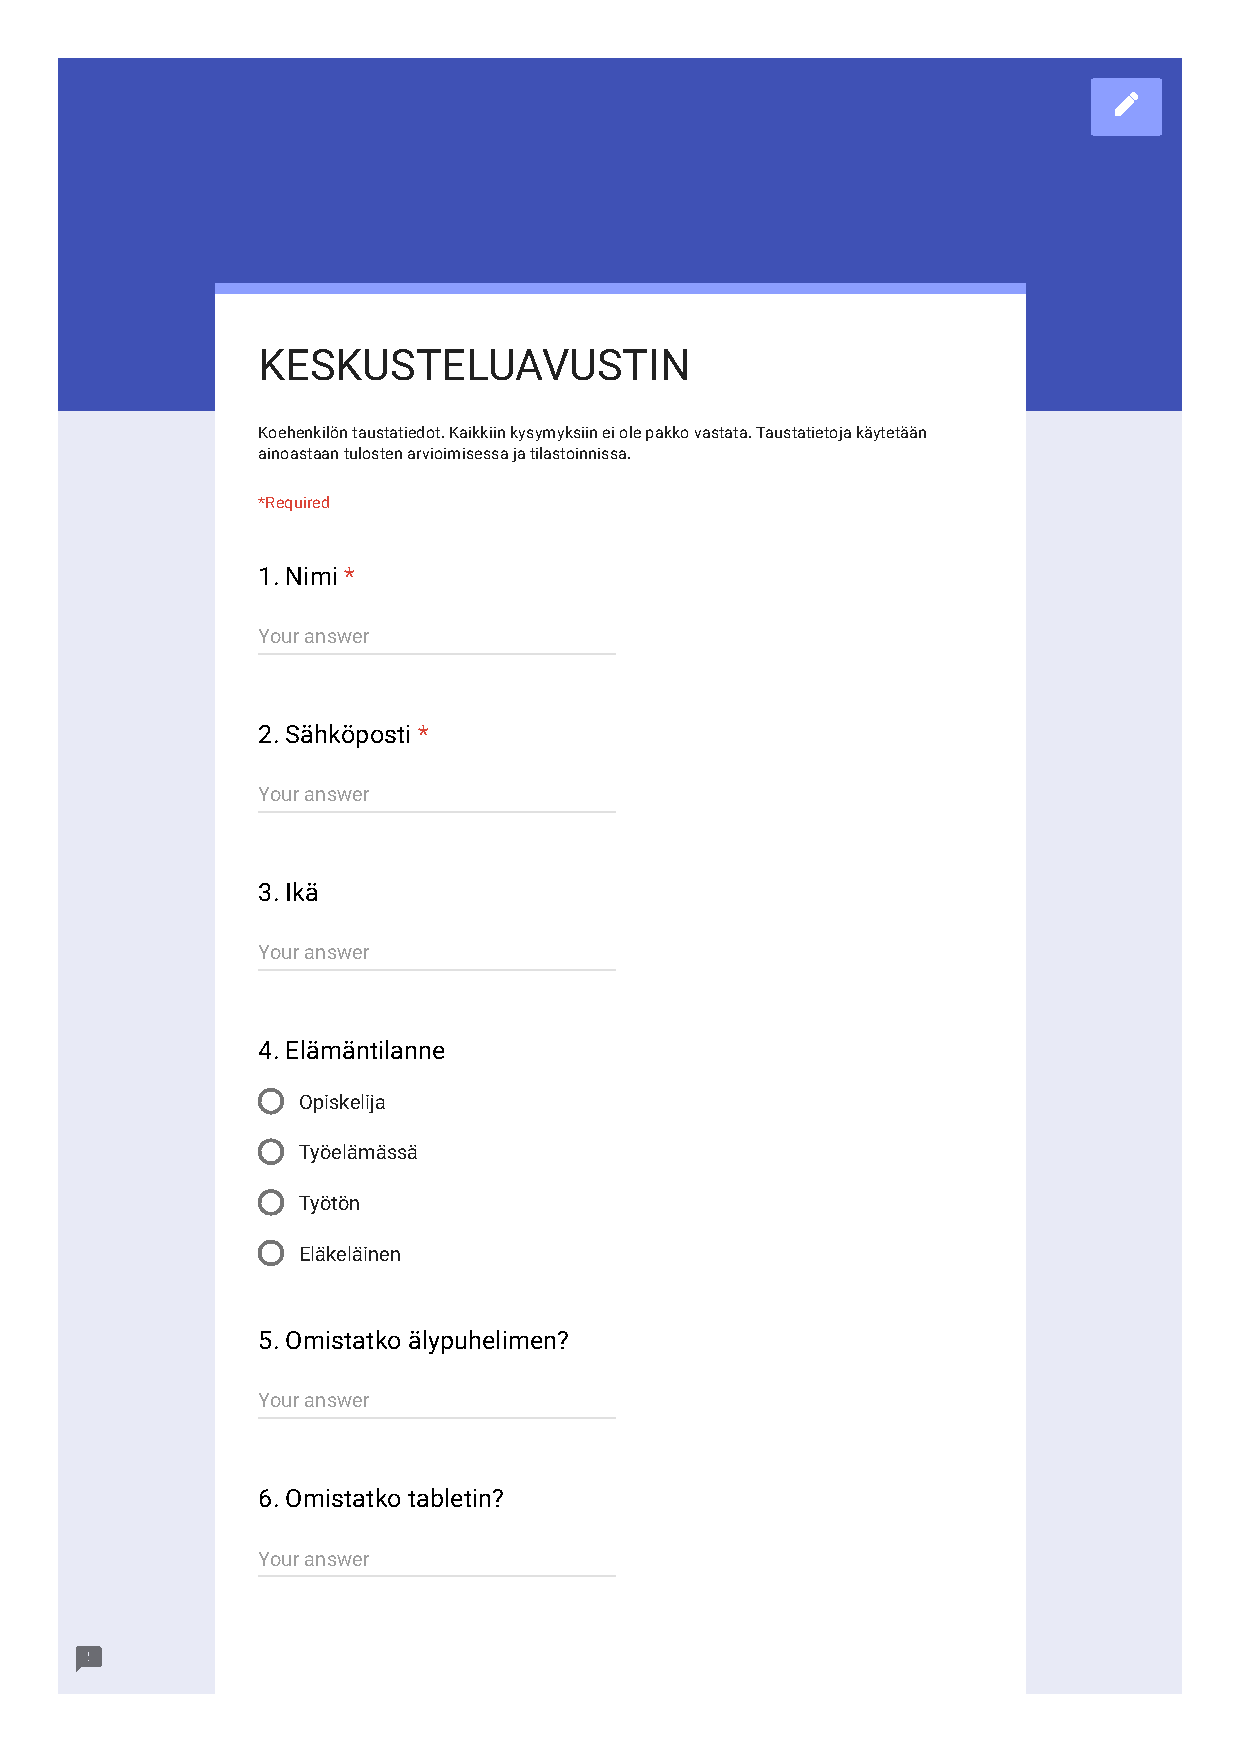
\includegraphics[page=1,trim={1cm 2cm 1cm 2.5cm}, clip, width=\textwidth]{q1.pdf}
\end{figure}
\begin{figure}
    \centering
    \includegraphics[page=2,trim={1cm 0cm 1cm 0cm}, clip, width=\textwidth]{q1.pdf}
\end{figure}

\begin{figure}
    \centering
    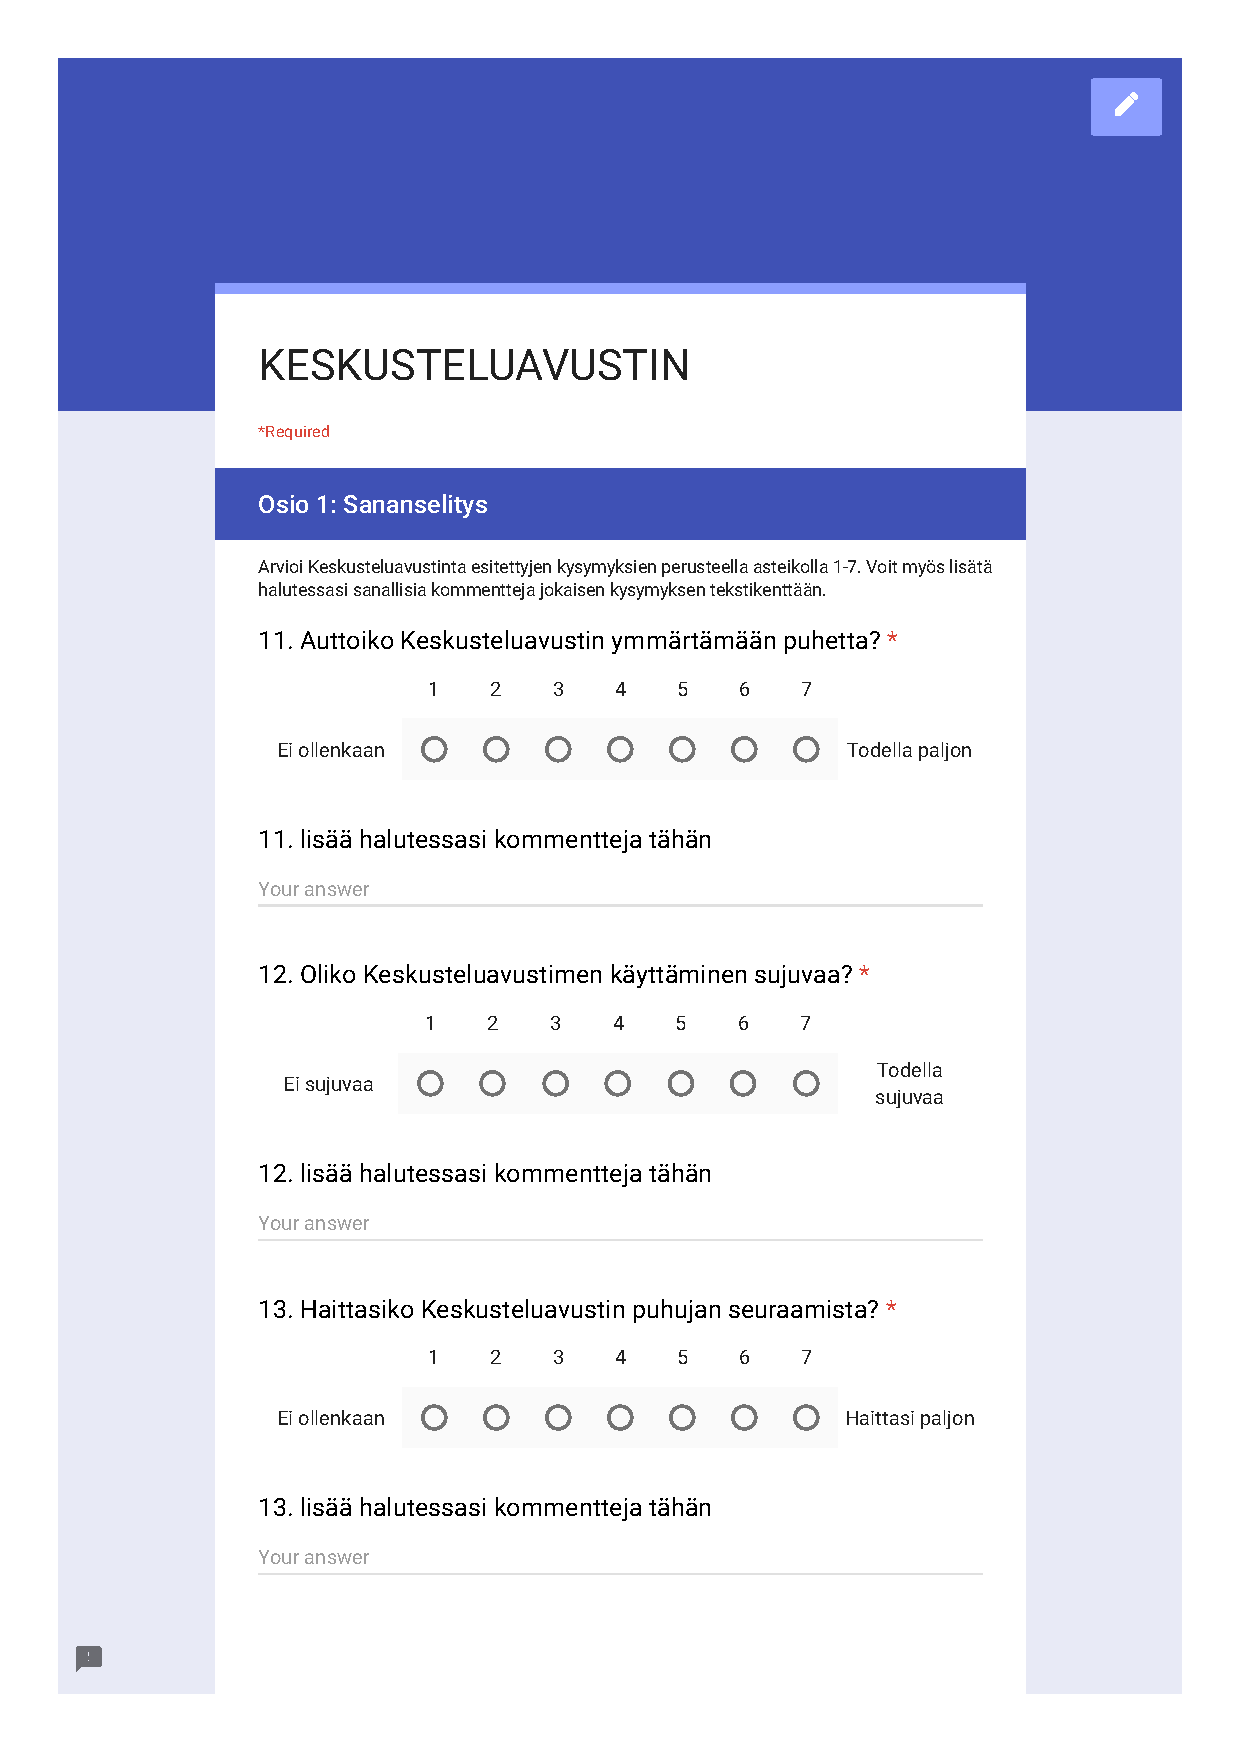
\includegraphics[page=1,trim={1cm 1cm 1cm 2.5cm}, clip, width=\textwidth]{q2.pdf}
\end{figure}
\begin{figure}
    \centering
    \includegraphics[page=2,trim={1cm 0cm 1cm 0cm}, clip, width=\textwidth]{q2.pdf}
\end{figure}

\begin{figure}
    \centering
    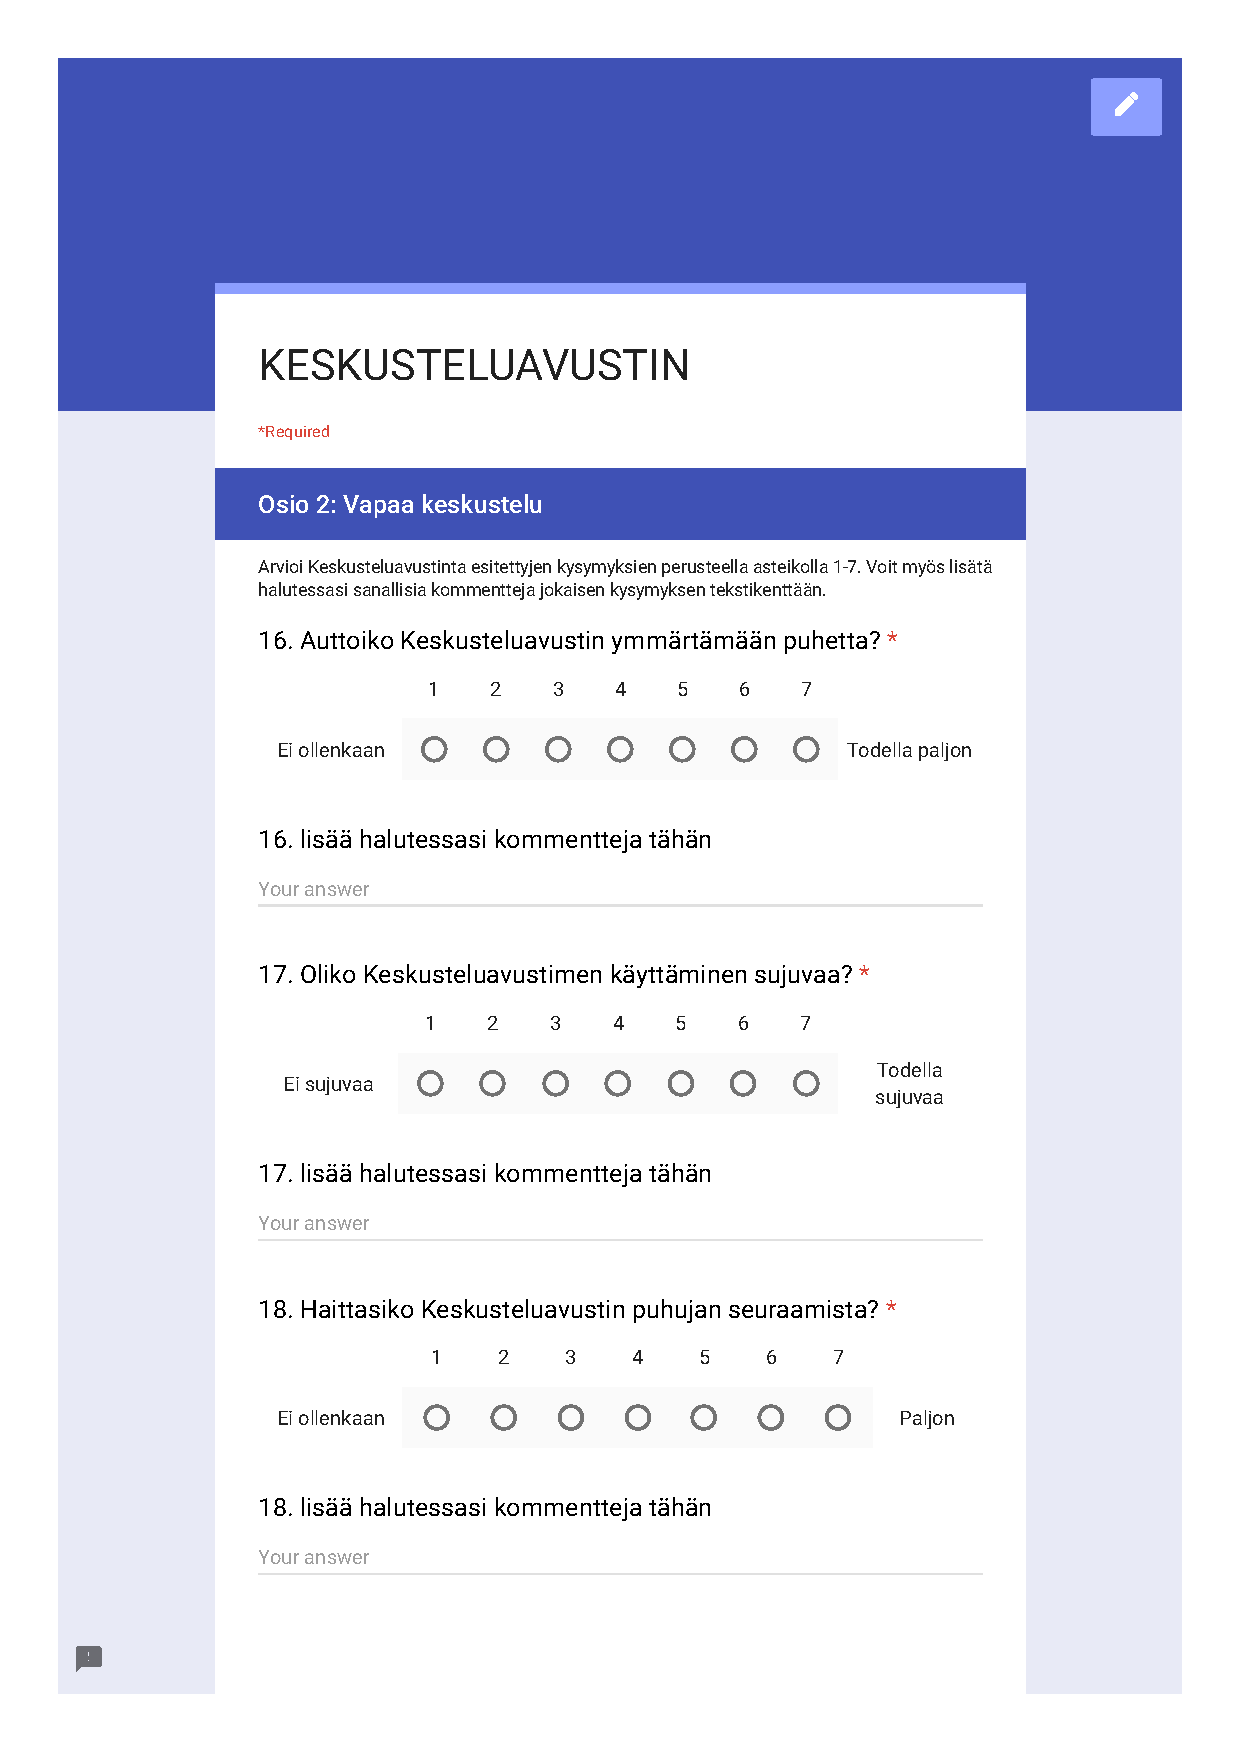
\includegraphics[page=1,trim={1cm 1cm 1cm 2.5cm}, clip, width=\textwidth]{q3.pdf}
\end{figure}
\begin{figure}
    \centering
    \includegraphics[page=2,trim={1cm 0cm 1cm 0cm}, clip, width=\textwidth]{q3.pdf}
\end{figure}

\begin{figure}
    \centering
    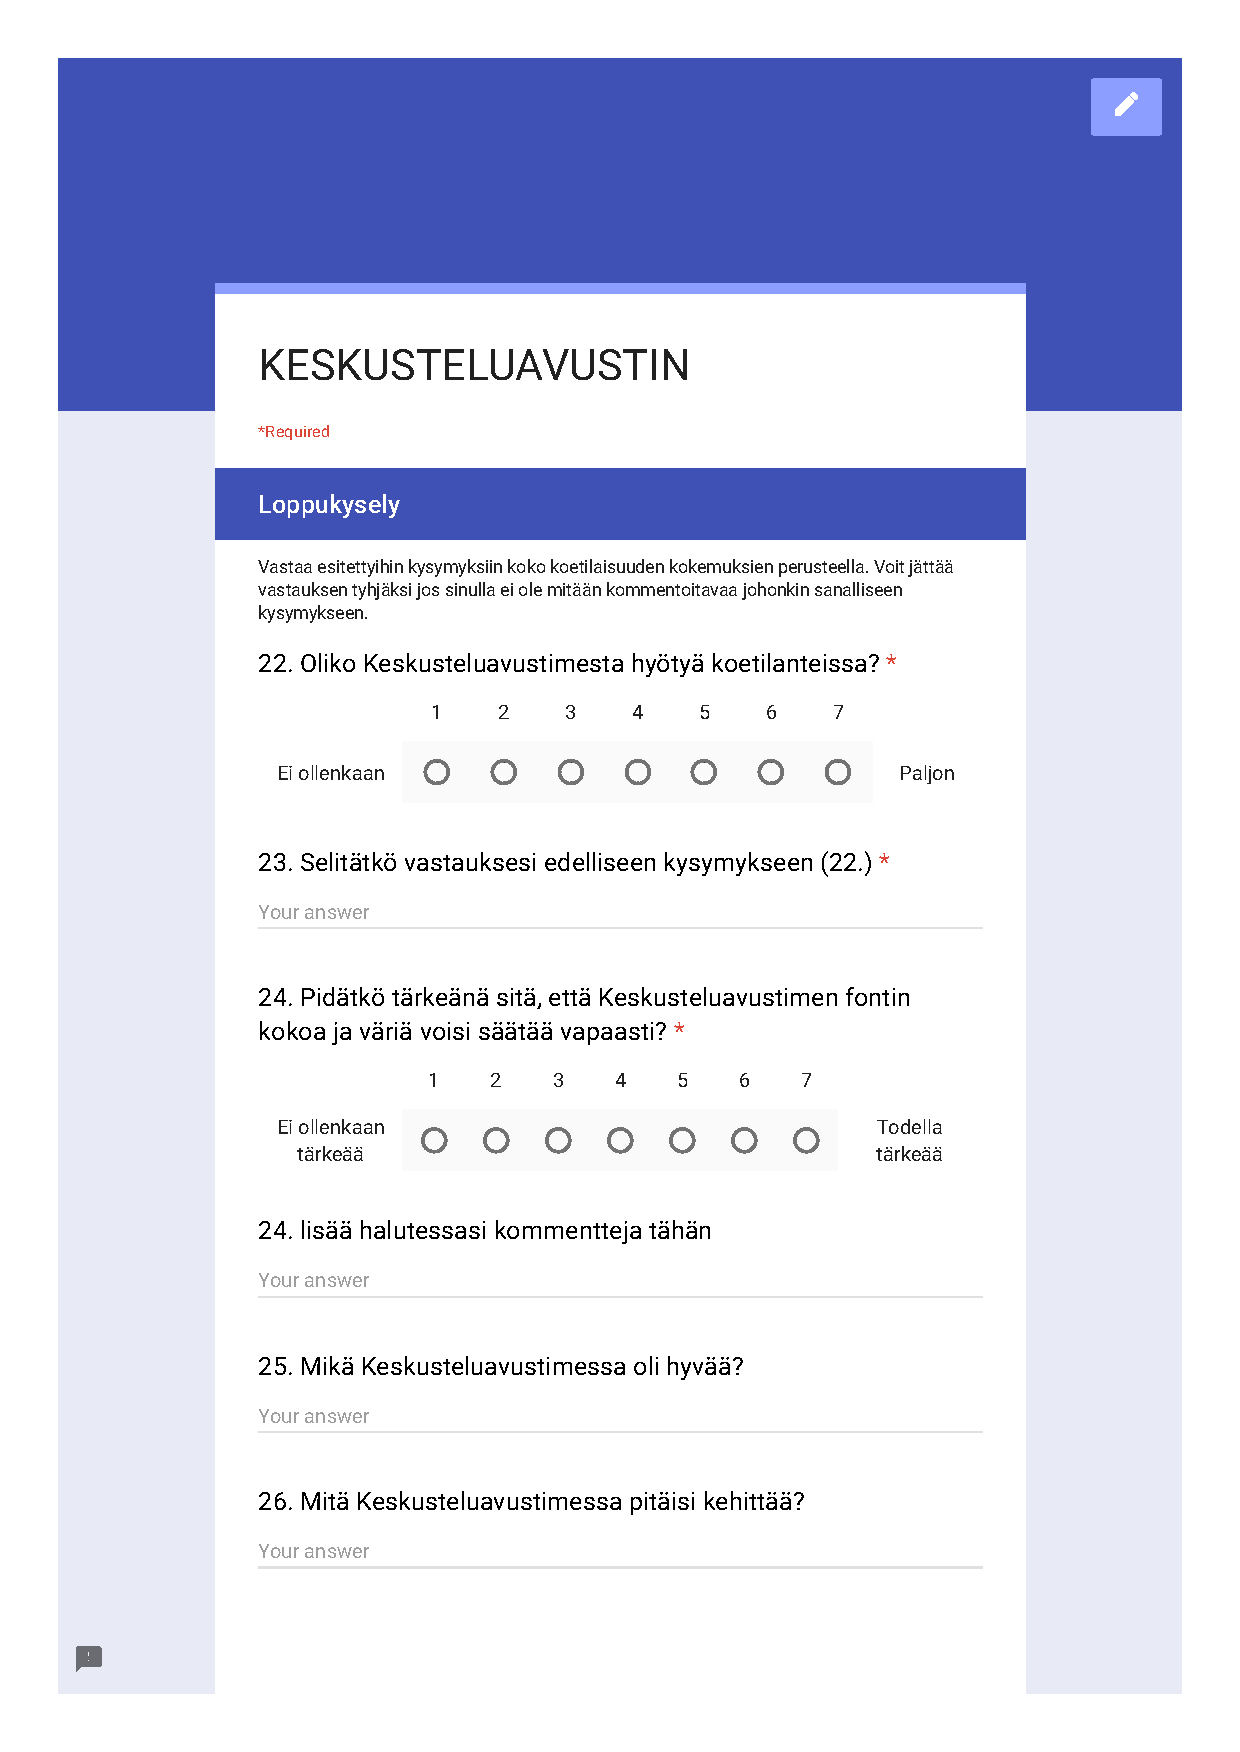
\includegraphics[page=1,trim={1cm 1cm 1cm 2.5cm}, clip, width=\textwidth]{q4.pdf}
\end{figure}
\begin{figure}
    \centering
    \includegraphics[page=2,trim={1cm 0cm 1cm 0cm}, clip, width=\textwidth]{q4.pdf}
\end{figure}
\begin{figure}
    \centering
    \includegraphics[page=3,trim={1cm 0cm 1cm 0cm}, clip, width=\textwidth]{q4.pdf}
\end{figure}

\section{Questionnaire Answers} \label{sec:answers}

The raw data from the user tests is included here. Each set of answers is identified by the number of the question, which corresponds to the number reported at the questionnaire listing in section \ref{sec:quest}. On the x-axis, P1 to P9 refer to the test participants. Values on the y-axis are the numerical answers on the scale from 1 to 7.

\begin{figure}[h!]
    \centering
    \begin{subfigure}[b]{0.49\textwidth}
        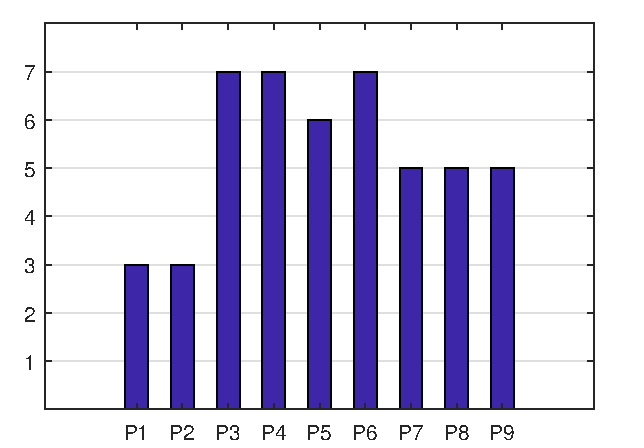
\includegraphics[width=\textwidth]{T2_1.pdf}
        \caption*{Q10}
    \end{subfigure}
    \begin{subfigure}[b]{0.49\textwidth}
        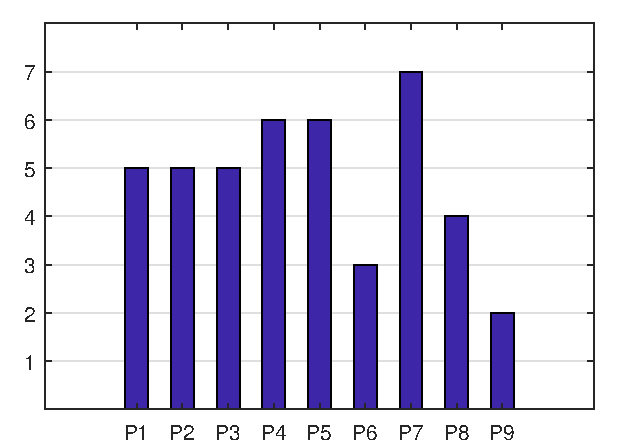
\includegraphics[width=\textwidth]{T2_2.pdf}
        \caption*{Q11}
    \end{subfigure}
    \begin{subfigure}[b]{0.49\textwidth}
        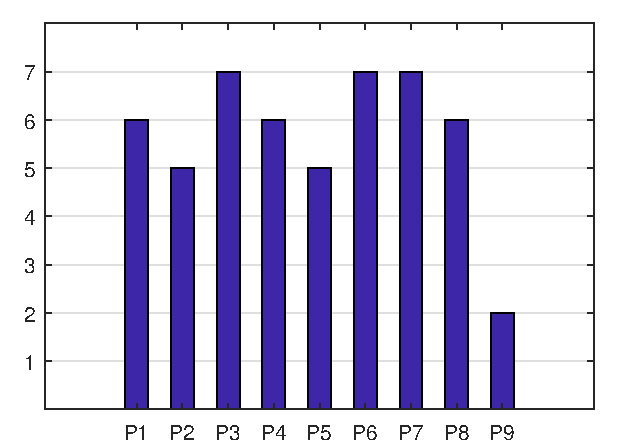
\includegraphics[width=\textwidth]{T2_3.pdf}
        \caption*{Q12}
    \end{subfigure}
    \begin{subfigure}[b]{0.49\textwidth}
        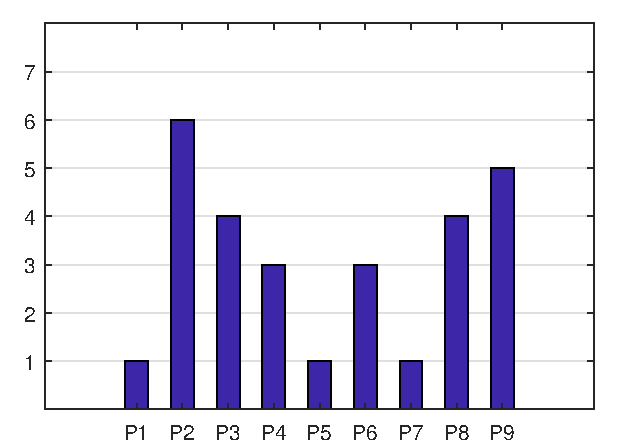
\includegraphics[width=\textwidth]{T2_4.pdf}
        \caption*{Q13}
    \end{subfigure}
    \begin{subfigure}[b]{0.49\textwidth}
        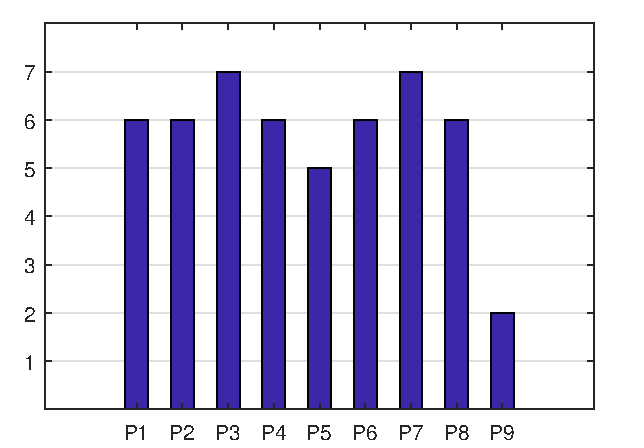
\includegraphics[width=\textwidth]{T2_5.pdf}
        \caption*{Q14}
    \end{subfigure}
    \begin{subfigure}[b]{0.49\textwidth}
        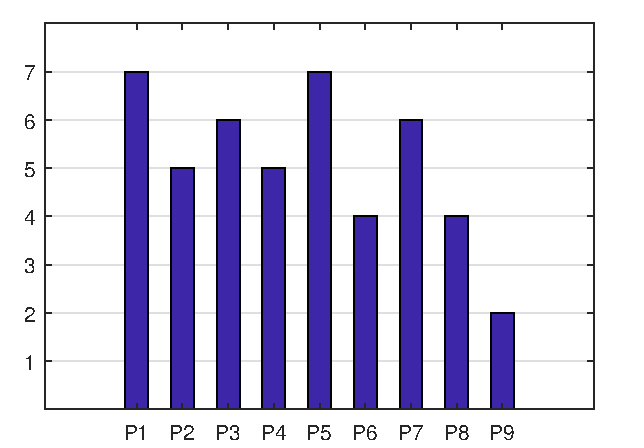
\includegraphics[width=\textwidth]{T2_6.pdf}
        \caption*{Q15}
    \end{subfigure}
    %\caption{Introduction and section 1 results.}
    %\label{fig:data} 
\end{figure}

\begin{figure}[h!]
    \centering
    \begin{subfigure}[b]{0.49\textwidth}
        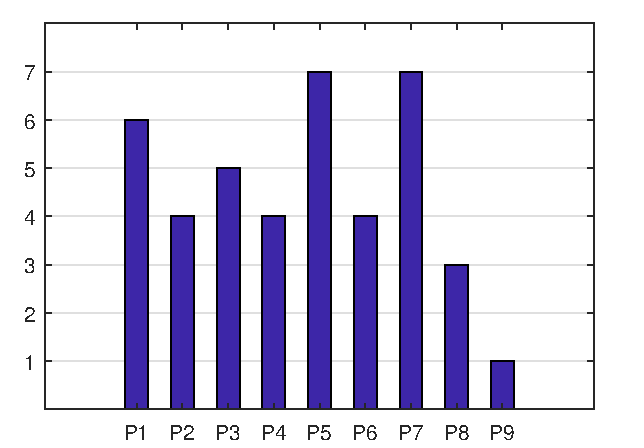
\includegraphics[width=\textwidth]{T2_7.pdf}
        \caption*{Q16}
    \end{subfigure}
    \begin{subfigure}[b]{0.49\textwidth}
        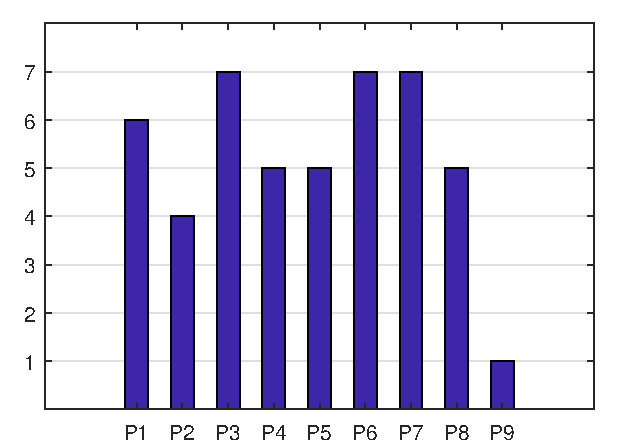
\includegraphics[width=\textwidth]{T2_8.pdf}
        \caption*{Q17}
    \end{subfigure}
    \begin{subfigure}[b]{0.49\textwidth}
        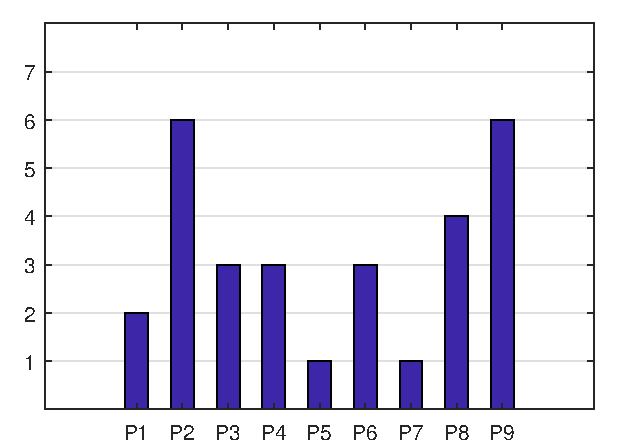
\includegraphics[width=\textwidth]{T2_9.pdf}
        \caption*{Q18}
    \end{subfigure}
    \begin{subfigure}[b]{0.49\textwidth}
        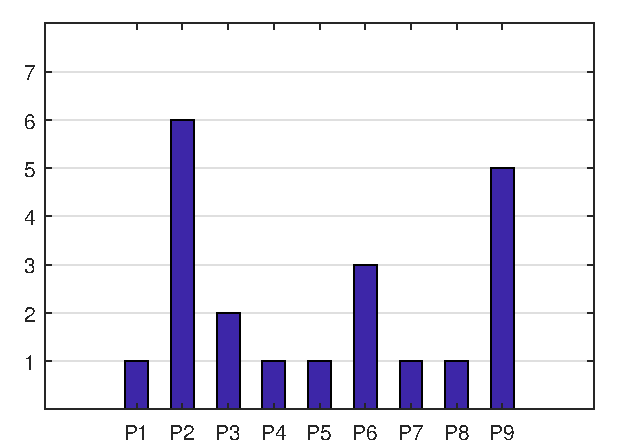
\includegraphics[width=\textwidth]{T2_10.pdf}
        \caption*{Q19}
    \end{subfigure}
    \begin{subfigure}[b]{0.49\textwidth}
        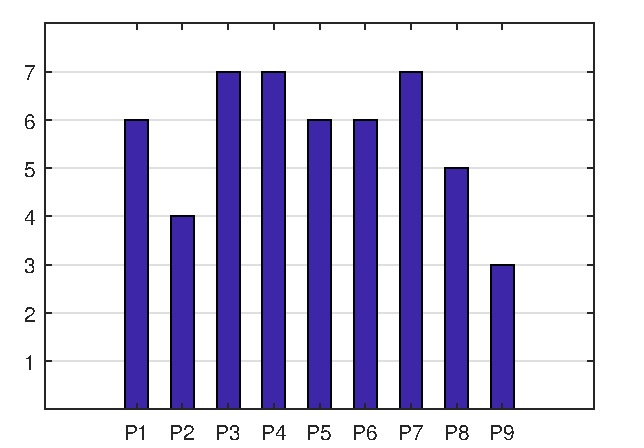
\includegraphics[width=\textwidth]{T2_11.pdf}
        \caption*{Q20}
    \end{subfigure}
    \begin{subfigure}[b]{0.49\textwidth}
        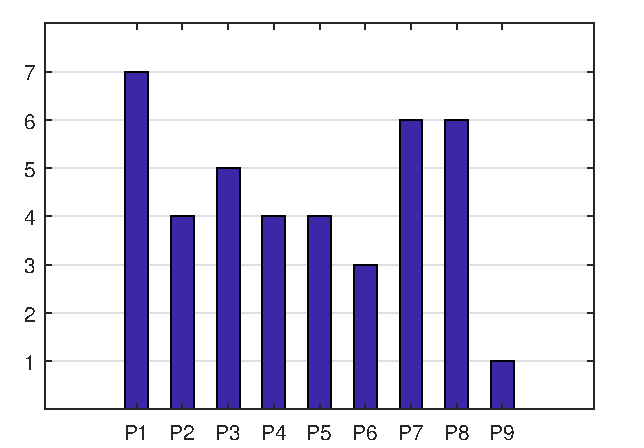
\includegraphics[width=\textwidth]{T2_12.pdf}
        \caption*{Q21}
    \end{subfigure}
    \begin{subfigure}[b]{0.49\textwidth}
        \includegraphics[width=\textwidth]{T2_13.pdf}
        \caption*{Q22}
    \end{subfigure}
    \begin{subfigure}[b]{0.49\textwidth}
        \includegraphics[width=\textwidth]{T2_14.pdf}
        \caption*{Q23}
    \end{subfigure}
    %\caption{Section 2 and debriefing results.}
    %\label{fig:data2} 
\end{figure}

\clearpage

%\section{MATLAB Code} \label{sec:matlab}

%This section presents the MATLAB scripts created for analyzing the user test results and producing most of the figures presented in this thesis.

%\lstset{
%   language=matlab,
%   basicstyle=\ttfamily\scriptsize, % \tiny 
%   inputencoding=utf8,
%   extendedchars=true,
%}

%\subsection*{results.m}
%\vspace{-4mm}
%\lstinputlisting{results.m}
%\vspace{8mm}
%\subsection*{audiosignal.m}
%\vspace{-4mm}
%\lstinputlisting{audiosignal.m}
%\vspace{8mm}
%\subsection*{bformat.m}
%\vspace{-4mm}
%\lstinputlisting{bformat.m}
%\vspace{8mm}
%\subsection*{cepstrum.m}
%\vspace{-4mm}
%\lstinputlisting{cepstrum.m}
%\vspace{8mm}
%\subsection*{gmm.m}
%\vspace{-4mm}
%\lstinputlisting{gmm.m}
%\vspace{8mm}
%\subsection*{filterbank.m}
%\vspace{-4mm}
%\lstinputlisting{filterbank.m}
%\vspace{8mm}
%\subsection*{loudness.m}
%\vspace{-4mm}
%\lstinputlisting{loudness.m}

\end{document}
